\documentclass[10pt,a4paper]{article}
\usepackage[T1]{fontenc}
\usepackage[utf8]{inputenc}
\usepackage{lmodern,amsmath,amssymb,mathrsfs,tikz-cd,microtype}
\usepackage[margin=17mm,footskip=8mm]{geometry}
\usepackage{booktabs,longtable,array,tabularx,calc,adjustbox}
\usepackage{fancyhdr}
\usepackage[unicode,hidelinks,bookmarks=false]{hyperref}
\setcounter{secnumdepth}{-10}
\pdfinfoomitdate=1
\pdftrailerid{}
\pdfsuppressptexinfo=15
\pagestyle{fancy}
\fancyhf{}
\renewcommand{\headrulewidth}{0pt}
\fancyfoot[C]{\thepage}
\setlength{\parindent}{1em}
\setlength{\parskip}{2pt}
\setlength{\emergencystretch}{4em}
\DeclareUnicodeCharacter{03A8}{\ensuremath{\Psi}}
\DeclareUnicodeCharacter{03C6}{\ensuremath{\varphi}}
\DeclareUnicodeCharacter{03B1}{\ensuremath{\alpha}}
\DeclareUnicodeCharacter{03A3}{\ensuremath{\Sigma}}
\DeclareUnicodeCharacter{03C1}{\ensuremath{\rho}}
\DeclareUnicodeCharacter{03C0}{\ensuremath{\pi}}
\DeclareUnicodeCharacter{03BC}{\ensuremath{\mu}}
\DeclareUnicodeCharacter{03C3}{\ensuremath{\sigma}}
\DeclareUnicodeCharacter{03C4}{\ensuremath{\tau}}
\DeclareUnicodeCharacter{03C9}{\ensuremath{\omega}}
\DeclareUnicodeCharacter{03B3}{\ensuremath{\gamma}}
\DeclareUnicodeCharacter{0393}{\ensuremath{\Gamma}}
\DeclareUnicodeCharacter{0394}{\ensuremath{\Delta}}
\DeclareUnicodeCharacter{2192}{\ensuremath{\to}}
\DeclareUnicodeCharacter{2032}{\ensuremath{{}^{\prime}}}
\DeclareUnicodeCharacter{2033}{\ensuremath{{}^{\prime\prime}}}
\DeclareUnicodeCharacter{2080}{\ensuremath{{}_0}}
\DeclareUnicodeCharacter{2081}{\ensuremath{{}_1}}
\DeclareUnicodeCharacter{2086}{\ensuremath{{}_6}}
\DeclareUnicodeCharacter{2087}{\ensuremath{{}_7}}
\DeclareUnicodeCharacter{2243}{\ensuremath{\simeq}}
\DeclareUnicodeCharacter{207A}{\ensuremath{{}^+}}
\DeclareUnicodeCharacter{2229}{\ensuremath{\cap}}
\DeclareUnicodeCharacter{2208}{\ensuremath{\in}}
\DeclareUnicodeCharacter{2212}{\ensuremath{-}}
\DeclareUnicodeCharacter{21A6}{\ensuremath{\mapsto}}
\DeclareUnicodeCharacter{1D516}{\ensuremath{\mathfrak S}}
\DeclareUnicodeCharacter{2265}{\ensuremath{\geq}}
\DeclareUnicodeCharacter{27E8}{\ensuremath{\langle}}
\DeclareUnicodeCharacter{27E9}{\ensuremath{\rangle}}
\DeclareUnicodeCharacter{2209}{\ensuremath{\notin}}
\DeclareUnicodeCharacter{2282}{\ensuremath{\subset}}
\DeclareUnicodeCharacter{2283}{\ensuremath{\supset}}
\DeclareUnicodeCharacter{2218}{\ensuremath{\circ}}
\providecommand{\tightlist}{\setlength{\itemsep}{0pt}\setlength{\parskip}{0pt}}
\providecommand{\passthrough}[1]{#1}
\newcommand{\SourcePage}[2]{\clearpage\setcounter{page}{#2}\typeout{D031_SOURCE_PAGE physical=#1 printed=#2}}
\begin{document}
\SourcePage{1}{247}
\section{SHIMURA VARIETIES: MODULAR INTERPRETATION AND TECHNIQUES FOR CONSTRUCTING CANONICAL MODELS}

PIERRE DELIGNE

\subsubsection{CONTENTS}

\begin{tabularx}{\linewidth}{@{}Xr@{}}
Introduction & 247 \\
Review, terminology and notation & 250 \\
1. Hermitian symmetric domains & 251 \\
1.1 Moduli spaces of Hodge structures & 251 \\
1.2 Classification & 257 \\
1.3 Symplectic embeddings & 259 \\
2. Shimura varieties & 262 \\
2.0 Preliminaries & 262 \\
2.1 Shimura varieties & 265 \\
2.2 Canonical models & 268 \\
2.3 Construction of canonical models & 270 \\
2.4 Reciprocity laws: preliminaries & 274 \\
2.5 Application: a canonical extension & 280 \\
2.6 The reciprocity law for canonical models & 284 \\
2.7 Reduction to the derived group, and existence theorem & 285 \\
Bibliography & 289 \\
\end{tabularx}

\textbf{Introduction.} This article is a sequel to {[}5{]}, whose essential results (those of sections 4 and 5) we shall use. In a first part, we attempt to motivate the axioms imposed on systems \((G,X)\) (2.1.1), from which Shimura varieties are defined. We show that, roughly speaking, they correspond to moduli spaces of Hodge structures \(X^+\) of the following kind.

\begin{enumerate}
\def\labelenumi{(\alph{enumi})}
\tightlist
\item
  \(X^+\) is a connected component of the space of all Hodge structures on a fixed vector space \(V\) for which certain tensors \(t_1\cdots t_n\) are of type \((0,0)\). The algebraic group \(G\) is the subgroup of \(\mathrm{GL}(V)\) fixing the \(t_i\), and \(X\) is the orbit \(G(\mathbf R)\cdot X^+\) of \(X^+\) under \(G(\mathbf R)\).
\end{enumerate}

\SourcePage{2}{248}
\begin{enumerate}
\def\labelenumi{(\alph{enumi})}
\setcounter{enumi}{1}
\tightlist
\item
  The family of Hodge structures on \(V\) parametrized by \(X^+\) satisfies certain conditions, which are satisfied by families of Hodge structures that occur naturally in algebraic geometry: for a suitable (and uniquely determined) complex structure on \(X^+\), it is a polarizable variation of Hodge structure.
\end{enumerate}

The space \(X^+\) is automatically a \emph{Hermitian symmetric domain} (= a Hermitian symmetric space of curvature \(<0\)). All Hermitian symmetric domains can be described in this way as moduli spaces of Hodge structures (1.1.17), and I believe this description to be very useful. For example, the embedding of a Hermitian symmetric domain \(D\) into its dual \(\check D\) (a flag variety) corresponds to the assignment (a Hodge structure) \(\mapsto\) (the corresponding Hodge filtration). Descriptions such as ``Siegel domain of the third kind'' are interpreted by saying that, under certain hypotheses, if one superimposes a weight filtration on a Hodge structure, one obtains a mixed Hodge structure, hence a map from \(D\) into a moduli space of mixed Hodge structures (cf.~the constructions of {[}1, III, 4.1{]}). This last point will neither be mentioned nor used in the article.

This viewpoint and the description of certain Shimura varieties as moduli spaces of abelian varieties are connected by the following dictionary: to give an abelian variety is equivalent (under the equivalence of categories \(A\mapsto H_1(A,\mathbf Z)\)) to giving a polarizable Hodge structure of type \(\{(-1,0),(0,-1)\}\) (here these are torsion-free \(\mathbf Z\)-Hodge structures; by passing to the dual, \((A\mapsto H^1(A,\mathbf Z))\), one may replace \(\{(-1,0),(0,-1)\}\) by \(\{(1,0),(0,1)\}\)). Polarizing the abelian variety amounts to polarizing its \(H_1\). With parameters, similarly, to give a polarized abelian scheme over a smooth complex variety \(S\) amounts to giving a polarized variation of Hodge structures of type \(\{(-1,0),(0,-1)\}\) on the analytic space \(S^{\mathrm{an}}\). An analytic family of abelian varieties parametrized by \(S^{\mathrm{an}}\) is automatically algebraic (this follows from {[}3{]}). To interpret Hodge structures of more complicated type, one would like to replace abelian varieties by suitable ``motives,'' but this is still only a dream.

In 1.2, we give a convenient description, based on the preceding formalism, of the classification of Hermitian symmetric domains in terms of Dynkin diagrams and their special vertices. In 1.3, we classify a certain kind of embedding of Hermitian symmetric domains into Siegel half-space. The results parallel those of Satake {[}11{]}. An application of Weyl's unitary trick, for which we refer to {[}7{]}, reduces the classification to knowledge of a fragment of the table, given for example in Bourbaki {[}4{]}, expressing the fundamental weights as linear combinations of simple roots.

The reader wishing to know more about variations of Hodge structure and how they arise in algebraic geometry may consult {[}6{]} (whose sign conventions we do not follow); certain facts stated in {[}6{]} are proved in {[}7{]}.

In 2.1 and 2.2 we define, in adelic language, the \emph{Shimura varieties} \({}_K M_{\mathbf C}(G,X)\) (denoted \({}_K M_{\mathbf C}(G,h)\) in {[}5{]}, for any \(h\in X\)), their projective limit \(M_{\mathbf C}(G,X)\), and the notion of a \emph{canonical model}. I refer to the text for these definitions and shall say only that a canonical model of

\SourcePage{3}{249}
\(M_{\mathbf C}(G,X)\) is a model of \(M_{\mathbf C}(G,X)\) over the \emph{reflex field} (2.2.1) \(E(G,X)\), that is, a scheme \(M(G,X)\) over \(E(G,X)\) equipped with an isomorphism

\[
M(G,X)\otimes_{E(G,X)}\mathbf C\;\xrightarrow{\sim}\;M_{\mathbf C}(G,X).
\]

This way of defining \(M_{\mathbf C}(G,X)\) over \(E(G,X)\) has the appropriate properties (\(G(A^f)\)-equivariance and Galois properties of the \emph{special points} (2.2.4)). We also define the notion of a weakly canonical model (the same definition as for canonical models, with \(E(G,X)\) replaced by a finite extension \(E\subset\mathbf C\)). Such models play a technical role in the construction of canonical models. The apparent differences between the definitions in 2.1 and 2.2 and those in {[}5{]} arise from a different choice of sign conventions (right action versus left action, the reciprocity law in global class field theory, and so on).

For a heuristic description, I refer to the introduction of {[}5{]}. For a brief description, by way of examples, of how one passes from adelic language to more classical language, I refer to {[}5, 1.6---1.11, 3.14---3.16, 4.11---4.16{]}.

In {[}5{]}, we systematized the methods introduced by Shimura for constructing canonical models. In the second part of the present article, we refine the results of {[}5{]}. In 2.6, we determine the action of the Galois group \(\mathrm{Gal}(\overline{\mathbf Q}/E)\) on the set of geometric connected components of a weakly canonical model (assumed to exist) of \(M_{\mathbf C}(G,X)\) over \(E\), without assuming, as in {[}5{]}, that the derived group of \(G\) is simply connected. The essential point is the construction, given in 2.4, of a morphism of the following kind. Let \(G\) be a (connected) reductive group over \(\mathbf Q\), let \(\rho:\widetilde G\to G\) be the universal covering of its derived group \(G^{\mathrm{der}}\), and let \(M\) be a conjugacy class, defined over a number field \(E\), of homomorphisms from \(G_m\) to \(G\). We construct a homomorphism \(q_M\) from the idèle class group of \(E\) into the abelian quotient \(G(A)/\rho\widetilde G(A)\cdot G(\mathbf Q)\) of \(G(A)\). This homomorphism is functorial in \((G,M)\) and, if \(F\) is an extension of \(E\), the diagram

\[
\begin{tikzcd}[column sep=large,row sep=normal]
C(F) \arrow[dd,"N_{F/E}"'] \arrow[dr] & \\
& G(A)/\rho\widetilde G(A)\cdot G(\mathbf Q) \\
C(E) \arrow[ur] &
\end{tikzcd}
\]

is commutative. If \(\widetilde G\) has no factor \(G'\) over \(\mathbf Q\) such that \(G'(\mathbf R)\) is compact, the strong approximation theorem gives

\[
\pi_0\bigl(G(A)/\rho\widetilde G(A)G(\mathbf Q)\bigr)
=
\pi_0\bigl(G(A)/G(\mathbf Q)\bigr),
\]

and \(q_M\) gives an action on \(\pi_0(G(A)/G(\mathbf Q))\) by \(\pi_0C(E)\), the abelianized Galois group \(\mathrm{Gal}(\overline{\mathbf Q}/E)^{\mathrm{ab}}\), according to global class field theory.

The second new idea---in fact, a return to Shimura's viewpoint---is the following observation: the results of 2.6 make it possible to reconstruct a weakly canonical model \(M_E(G,X)\) of \(M_{\mathbf C}(G,X)\) from its neutral component \(M^0_{\overline{\mathbf Q}}(G,X^+)\) (a geometric connected component, depending on the choice of a connected component \(X^+\) of \(X\)), equipped with the (semilinear) action of the subgroup \(H\) of \(G(A^f)\times\mathrm{Gal}(\overline{\mathbf Q}/E)\) that stabilizes it. Let \(Z\) be the center of \(G\), let \(G^{\mathrm{ad}}\) be the adjoint group, let \(G^{\mathrm{ad}}(\mathbf R)^+\) be the topological identity component of \(G^{\mathrm{ad}}(\mathbf R)\), and let \(G^{\mathrm{ad}}(\mathbf Q)^+=G^{\mathrm{ad}}(\mathbf Q)\cap G^{\mathrm{ad}}(\mathbf R)^+\). Since the closure \(Z(\mathbf Q)^-\) of \(Z(\mathbf Q)\) in \(G(A^f)\) acts trivially on \(M_{\mathbf C}(G,X)\), the ac-

\SourcePage{4}{250}
tion of \(H\) on \(M^0_{\overline{\mathbf Q}}(G,X^+)\) factors through \(H/Z(\mathbf Q)^-\). In fact, one can let a slightly larger group act: an extension of \(\mathrm{Gal}(\overline{\mathbf Q}/E)\) by the completion of \(G^{\mathrm{ad}}(\mathbf Q)^+\) for the topology defined by the images of the congruence subgroups of \(G^{\mathrm{der}}(\mathbf Q)\).

Up to unique isomorphism, this extension depends only on \(G^{\mathrm{ad}}\), \(G^{\mathrm{der}}\), and the projection \(X^{+\mathrm{ad}}\) of \(X^+\) into \(G^{\mathrm{ad}}\) (2.5). We denote it by \(\mathscr E_E(G^{\mathrm{ad}},G^{\mathrm{der}},X^{+\mathrm{ad}})\). The neutral component \(M^0_{\mathbf C}(G,X^+)\) is the projective limit of the quotients of \(X^{+\mathrm{ad}}\) by arithmetic subgroups of \(G^{\mathrm{ad}}(\mathbf Q)^+\) that are images of congruence subgroups of \(G^{\mathrm{der}}(\mathbf Q)\). Finally, one checks that the conditions to be satisfied by its model \(M^0_{\overline{\mathbf Q}}(G,X^+)\) over \(\overline{\mathbf Q}\), and by the action of \(\mathscr E_E(G^{\mathrm{ad}},G^{\mathrm{der}},X^{+\mathrm{ad}})\), in order to correspond to a weakly canonical model, depend only on the adjoint group \(G^{\mathrm{ad}}\), on \(X^{+\mathrm{ad}}\), on the covering \(G^{\mathrm{der}}\) of \(G^{\mathrm{ad}}\), and on the finite extension \(E\) (contained in \(\mathbf C\)) of \(E(G^{\mathrm{ad}},X^{+\mathrm{ad}})\). These conditions define the connected \emph{weakly canonical} models (respectively, the connected \emph{canonical} models when \(E=E(G^{\mathrm{ad}},X^{+\mathrm{ad}})\)) (2.7.10).

Thus, roughly speaking, the problem of the existence of a canonical model depends only on the derived group. This reduction to the derived group is a much more convenient version of the awkward method of central modification of \(h\) in {[}5, 5.11{]}.

In 2.3, we construct a supply of canonical models by means of symplectic embeddings, invoking {[}5, 4.21 and 5.7{]}. The results of 1.3 enable us to obtain the desired symplectic embeddings with very little calculation. In 2.7, we explain the reduction to the derived group sketched above and deduce from 2.3 a criterion for the existence of canonical models that covers all known cases (Shimura, Miyake, and Shih).

In this article, we use the equivalence between weakly canonical models and connected weakly canonical models to transfer to the latter certain results of {[}5{]} (uniqueness and the construction of a canonical model from a family of weakly canonical models). It would have been more natural to transpose the proofs, and likewise to transpose functoriality {[}5, 5.4{]} and passage to a subgroup {[}5, 5.7{]} (thereby avoiding the cryptic proposition {[}5, 1.15{]}). Lack of time and weariness prevented me from doing so.

I have recently proved that one can give a purely algebraic meaning to the notion of a rational cycle of type \((p,p)\) on an abelian variety \(A\) (over a field of characteristic 0). From this one can recover criterion 2.3.1 for the existence of canonical models and give a modular description of the models obtained with its help (cf.~{[}9{]}). Unfortunately, this description does not lend itself to reduction modulo \(p\). This method avoids recourse to {[}5, 5.7{]} (and thereby to {[}5, 1.15{]}) and gives partial information on the conjugation of Shimura varieties.

\subsection{0. Review, terminology and notation.}

\textbf{0.1.} We shall have occasion to use the strong approximation theorem, the real approximation theorem, the Hasse principle, and the vanishing of \(H^1(K,G)\) for \(G\) semisimple and simply connected over a nonarchimedean local field. Bibliographic references for these theorems are given in {[}5, (0.1) to (0.4){]}. We also mention the article of G. Prasad, \emph{Strong approximation for semi-simple groups over function fields}, Ann. of Math. (2) 105 (1977), 553--572, which proves the strong approximation theorem over an arbitrary global field. Let \(G\) be a semisimple simply connected group with center \(Z\) over a global field \(K\). We shall use

\SourcePage{5}{251}
the Hasse principle for \(H^1(K,G)\) only for classes in the image of \(H^1(K;Z)\). In particular, the \(E_8\) factors are irrelevant to us.

\textbf{0.2.} \emph{Reductive group} will always mean \emph{connected reductive group}. A \emph{covering} of a reductive group is a \emph{connected} covering. \emph{Adjoint group} will mean \emph{reductive adjoint group}. If \(G\) is a reductive group, we denote its adjoint group by \(G^{\mathrm{ad}}\), its derived group by \(G^{\mathrm{der}}\), and the universal covering of \(G^{\mathrm{der}}\) by \(\rho:\widetilde G\to G^{\mathrm{der}}\). We often denote the center of \(G\) by \(Z\) (or \(Z(G)\)), and, by a conflict of notation, the center of \(\widetilde G\) by \(\widetilde Z\).

\textbf{0.3.} A superscript \(0\) will denote an \emph{algebraic connected component} (for example, \(Z^0\) is the identity component of the center \(Z\) of \(G\)). A superscript \(+\) will denote a \emph{topological connected component} (for example, \(G(\mathbf R)^+\) is the topological identity component of the group of real points of a group \(G\)). We also write \(G(\mathbf Q)^+\) for the trace of \(G(\mathbf R)^+\) on \(G(\mathbf Q)\). For a real reductive group \(G\), a subscript \(+\) will denote the inverse image of \(G^{\mathrm{ad}}(\mathbf R)^+\) in \(G(\mathbf R)\). We use the same subscript notation for the trace on a group of rational points.

For a topological space \(X\), we denote by \(\pi_0(X)\) the set of its connected components, endowed with the quotient topology from \(X\). In this article, \(\pi_0(X)\) will always be discrete or compact and totally disconnected.

\textbf{0.4.} A \emph{Hermitian symmetric domain} is a Hermitian symmetric space of curvature \(<0\) (that is, with no Euclidean or compact factor).

\textbf{0.5.} Unless expressly stated otherwise, a \emph{vector space} is assumed finite-dimensional, and a \emph{number field} is assumed to have finite degree over \(\mathbf Q\). The number fields we consider will most often be contained in \(\mathbf C\); \(\overline{\mathbf Q}\) denotes the algebraic closure of \(\mathbf Q\) in \(\mathbf C\).

\textbf{0.6.} Put \(\widehat{\mathbf Z}=\varprojlim \mathbf Z/n\mathbf Z=\prod_p\mathbf Z_p\) and \(A^f=\mathbf Q\otimes\widehat{\mathbf Z}=\prod_p'\mathbf Q_p\) (restricted product), and write \(A=\mathbf R\times A^f\) for the ring of adèles of \(\mathbf Q\). We shall sometimes also write \(A\) for the ring of adèles of an arbitrary global field.

\textbf{0.7.} \(G(K)\), \(G\otimes_FK\), \(G_K\): if \(G\) is a scheme over \(F\) (for example, an algebraic group over \(F\)) and \(K\) is an \(F\)-algebra, then \(G(K)\) denotes the set of \(K\)-valued points of \(G\), while \(G_K\) or \(G\otimes_FK\) denotes the scheme over \(K\) obtained from \(G\) by extension of scalars.

\textbf{0.8.} We normalize the reciprocity isomorphism of global class field theory (= choose it or its inverse)

\[
\pi_0 A_E^*/E^*\;\xrightarrow{\sim}\;\mathrm{Gal}(\overline{\mathbf Q}/E)^{\mathrm{ab}}
\]

so that the class of the idèle equal to a uniformizer at \(v\) and to 1 at all other places corresponds to a geometric Frobenius (the inverse of a Frobenius substitution) (cf.~1.1.6 and the justification loc. cit. 3.6, 8.12).

\subsection{1. Hermitian symmetric domains.}

\subsubsection{1.1. Moduli spaces of Hodge structures.}

\textbf{1.1.1.} Recall that a Hodge structure on a real vector space \(V\) is a bigrading \(V_{\mathbf C}=\bigoplus V^{pq}\) of the complexification of \(V\), such that \(V^{pq}\) is the complex conjugate of \(V^{qp}\).

Define an action \(h\) of \(\mathbf C^*\) on \(V_{\mathbf C}\) by

\[
\tag{1.1.1.1}
h(z)v=z^{-p}\bar z^{-q}v\qquad\text{for }v\in V^{pq}.
\]

The \(h(z)\) commute with complex conjugation on \(V_{\mathbf C}\), and hence arise by ex-

\SourcePage{6}{252}
tension of scalars from an action, again denoted \(h\), of \(\mathbf C^*\) on \(V\). Regard \(\mathbf C\) as an extension of \(\mathbf R\), and let \(S\) be its multiplicative group, viewed as a real algebraic group (in other words, \(S=R_{\mathbf C/\mathbf R}G_m\), restriction of scalars in the sense of Weil); then \(S(\mathbf R)=\mathbf C^*\), and \(h\) is an action of the algebraic group \(S\). This construction defines an equivalence of categories: (real vector spaces equipped with a Hodge structure) \(\to\) (real vector spaces equipped with an action of the real algebraic group \(S\)).

The inclusion \(\mathbf R^*\subset\mathbf C^*\) corresponds to an inclusion of real algebraic groups \(G_m\subset S\). We denote by \(w_h\) (or simply \(w\)) the restriction of \(h^{-1}\) to \(G_m\), and call it the \emph{weight}, \(w:G_m\to\mathrm{GL}(V)\). We say that \(V\) is homogeneous of weight \(n\) if \(V^{pq}=0\) for \(p+q\ne n\), that is, if \(w(\lambda)\) is scalar multiplication by \(\lambda^n\).

We denote by \(\mu_h\) (or simply \(\mu\)) the action of \(G_m\) on \(V_{\mathbf C}\) defined by \(\mu(z)v=z^{-p}v\) for \(v\in V^{pq}\). It is the composite \(G_m\to S_{\mathbf C}\xrightarrow{h}\mathrm{GL}(V_{\mathbf C})\).

The \emph{Hodge filtration} \(F_h\) (or simply \(F\)) is defined by \(F^p=\bigoplus_{r\ge p}V^{rs}\). We say that \(V\) is of \emph{type} \(\mathscr C\subset\mathbf Z\times\mathbf Z\) if \(V^{pq}=0\) for \((p,q)\notin\mathscr C\).

More generally, if \(A\) is a subring of \(\mathbf R\) such that \(A\otimes\mathbf Q\) is a field (in practice, \(A=\mathbf Z\), \(\mathbf Q\), or \(\mathbf R\)), an \emph{\(A\)-Hodge structure} is a finite-type \(A\)-module \(V\) equipped with a Hodge structure on \(V\otimes_A\mathbf R\).

\textbf{EXAMPLE 1.1.2.} The fundamental example is \(V=H^n(X,\mathbf R)\), where \(X\) is a compact Kähler variety and \(V^{pq}\subset H^n(X,\mathbf C)\) is the space of cohomology classes represented by a closed form of type \((p,q)\). Other useful examples are obtained from this one by tensor products, by passage to a direct-summand Hodge structure, or by passage to the dual. Thus the dual \(H_n(X,\mathbf R)\) of \(H^n(X,\mathbf R)\) carries a Hodge structure of weight \(-n\). Integral homology or cohomology furnishes \(\mathbf Z\)-Hodge structures.

\textbf{EXAMPLE 1.1.3.} Hodge structures of type \(\{(-1,0),(0,-1)\}\) are those for which the action \(h\) of \(\mathbf C^*=S(\mathbf R)\) is induced by a complex structure on \(V\); for \(V\) of this type, the projection \(\operatorname{pr}\) from \(V\) onto \(V^{-1,0}\subset V_{\mathbf C}\) is bijective and satisfies \(\operatorname{pr}(h(z)v)=z\operatorname{pr}(v)\).

\textbf{EXAMPLE 1.1.4.} Let \(A\) be a complex torus; it is the quotient \(L/\Gamma\) of its Lie algebra \(L\) by a lattice \(\Gamma\). We have \(\Gamma\otimes\mathbf R\xrightarrow{\sim}L\), hence a complex structure on \(\Gamma\otimes\mathbf R\). Regard this as a Hodge structure (1.1.3). Via the isomorphism \(\Gamma=H_1(A,\mathbf Z)\), it is the structure of 1.1.2.

\textbf{EXAMPLE 1.1.5.} The Tate Hodge structure \(\mathbf Z(1)\) is the \(\mathbf Z\)-Hodge structure of type \((-1,-1)\) with integral lattice \(2\pi i\mathbf Z\subset\mathbf C\). The exponential identifies \(\mathbf C^*\) with \(\mathbf C/\mathbf Z(1)\), giving an isomorphism \(\mathbf Z(1)=H_1(\mathbf C^*)\). The Hodge structure \(\mathbf Z(n)\stackrel{\mathrm{dfn}}{=}\mathbf Z(1)^{\otimes n}\) \((n\in\mathbf Z)\) is the \(\mathbf Z\)-Hodge structure of type \((-n,-n)\) with integral lattice \((2\pi i)^n\mathbf Z\). We write \(\ldots(n)\) for the tensor product of \(\ldots\) with \(\mathbf Z(n)\) (the \emph{Tate twist}).

\textbf{1.1.6. REMARK.} The rule \(h(z)v=z^{-p}\bar z^{-q}v\) for \(v\in V^{pq}\) is the one I use in \emph{Les constantes des équations fonctionnelles des fonctions L}, Anvers II, Lecture Notes in Math., vol.~349, pp.~501--597, and is the inverse of the convention in {[}6{]}. It is justified, on the one hand, by Example 1.1.4 above, and, on the other, by the desire that \(\mathbf C^*\) act on \(\mathbf R(1)\) by multiplication by the norm (cf.~loc. cit., end of 8.12).

\textbf{1.1.7.} A \emph{variation of Hodge structure} on a complex analytic variety \(S\) consists of

\begin{enumerate}
\def\labelenumi{(\alph{enumi})}
\tightlist
\item
  a local system \(V\) of real vector spaces;
\end{enumerate}

\SourcePage{7}{253}
\begin{enumerate}
\def\labelenumi{(\alph{enumi})}
\setcounter{enumi}{1}
\tightlist
\item
  at each point \(s\) of \(S\), a Hodge structure on the fiber of \(V\) at \(s\), varying continuously with \(s\).
\end{enumerate}

We require that the Hodge filtration vary holomorphically with \(s\) and satisfy the axiom called \emph{transversality}: the derivative of a section of \(F^p\) lies in \(F^{p-1}\).

There will often be given a local system \(V_{\mathbf Z}\) of finitely generated \(\mathbf Z\)-modules such that \(V=V_{\mathbf Z}\otimes\mathbf R\). We shall then speak of a \emph{variation of} \(\mathbf Z\)-\emph{Hodge structure}. Likewise with \(\mathbf Z\) replaced by a ring \(A\) as in 1.1.1.

\textbf{1.1.8. REMARK.} Regard \(S\) as a real variety whose tangent space at each point is endowed with a complex structure, i.e.~a Hodge structure of type \(\{(-1,0),(0,-1)\}\). The integrability of the almost complex structure on \(S\) is expressed by saying that the bracket of vector fields is compatible with the Hodge filtration of the complexified tangent bundle:

\[
[T^{0,-1},T^{0,-1}]\subset T^{0,-1}.
\]

Similarly, the axiom for variations of Hodge structure says that the derivation

\[
(\text{tangent fiber})\otimes_{\mathbf R}(C^\infty\text{ sections of }V)
\longrightarrow
(C^\infty\text{ sections of }V)
\]

(or rather the complexification of this map) is compatible with the Hodge filtrations: \(\partial_DF^p\subset F^p\) for \(D\) in \(T^{0,-1}\) (holomorphicity), and \(\partial_DF^p\subset F^{p-1}\) for arbitrary \(D\) (transversality).

\textbf{PRINCIPLE 1.1.9.} In algebraic geometry, whenever a Hodge structure depending on complex parameters occurs, it is a variation of Hodge structure on the parameter space. The fundamental example is 1.1.2 with parameters: if \(f:X\to S\) is a smooth proper morphism with Kähler fibers \(X_s\), then the \(H^n(X_s,\mathbf Z)\) form a local system on \(S\), and the Hodge filtration on the complexification \(H^n(X_s,\mathbf C)\) varies holomorphically with \(s\) and satisfies the transversality axiom.

\textbf{1.1.10.} A \emph{polarization} of a real Hodge structure \(V\) of weight \(n\) is a morphism \(\Psi:V\otimes V\to\mathbf R(-n)\) such that the form \((2\pi i)^n\Psi(x,h(i)y)\) is symmetric and positive definite. Likewise for \(\mathbf Z\)-Hodge structures, replacing \(\mathbf R(-n)\) by \(\mathbf Z(-n)\), \ldots{} . Since \(\Psi(h(i)x,y)=\Psi(x,h(-i)y)\) (\(h(i)\) is trivial on \(\mathbf R(-n)\)), and since \(h(-i)y=(-1)^nh(i)y\), the symmetry condition amounts to this: \(\Psi\) is symmetric when \(n\) is even and alternating when \(n\) is odd.

The Hodge structures that occur in algebraic geometry are homogeneous and polarizable \(\mathbf Z\)-Hodge structures. The fundamental example is that the Hodge positivity theorems ensure that \(H^n(X,\mathbf Z)\) is polarizable when \(X\) is a smooth projective variety (note that \(h(i)\) is the operation denoted \(C\) by Weil in his book on Kähler varieties).

\textbf{1.1.11.} Let \((V_i)_{i\in I}\) be real vector spaces and let \((s_j)_{j\in J}\) be a family of tensors in tensor products of tensor powers of the \(V_i\) and their duals. We are interested in families of Hodge structures on the \(V_i\) for which the \(s_j\) are of type \((0,0)\). To interpret the condition ``type \((0,0)\)'' in particular cases, note that \(f:V\to W\) is a morphism if and only if, as an element of \(\operatorname{Hom}(V,W)=V^*\otimes W\), it is of type \((0,0)\).

Let \(G\) be the algebraic subgroup of \(\prod\operatorname{GL}(V_i)\) that fixes the \(s_j\). By 1.1.1, a family of Hodge structures on the \(V_i\) is identified with a morphism \(h:S\to\prod\operatorname{GL}(V_i)\). For the \(s_j\) to be of type \((0,0)\), it is necessary and sufficient that \(h\) factor through \(G\): one is to consider algebraic morphisms \(h:S\to G\).

One may regard \(G\), rather than the system of the \(V_i\) and \(s_j\), as the primary object: if \(G\) is a real linear algebraic group, it amounts to the same thing to give \(h:S\to\)

\SourcePage{8}{254}
\(G\), or to give on every representation \(V\) of \(G\) a Hodge structure, functorially for \(G\)-morphisms and compatibly with tensor products (cf.~Saavedra, {[}10, VI, §2{]}). The morphisms \(w_h\) and \(\mu_h\) of 1.1.1 become morphisms from \(G_m\) to \(G\) and from \(G_m\) to \(G_{\mathbf C}\), respectively.

\textbf{1.1.12.} Construction 1.1.11 leads us to consider moduli spaces of Hodge structures of the following kind: fix a real linear algebraic group \(G\), and consider a (topological) connected component \(X\) of the space of morphisms (= homomorphisms of algebraic groups over \(\mathbf R\)) from \(S\) to \(G\).

Let \(G_1\) be the smallest algebraic subgroup of \(G\) through which the \(h\in X\) factor: \(X\) is still a connected component of the space of morphisms from \(S\) to \(G_1\). Since \(S\) is of multiplicative type, any two elements of \(X\) are conjugate: the space \(X\) is a \(G_1(\mathbf R)^+\)-conjugacy class of morphisms from \(S\) to \(G\). It is also a \(G(\mathbf R)^+\)-conjugacy class, and \(G_1\) is a subgroup invariant under the identity component of \(G\).

\textbf{1.1.13.} In view of 1.1.9 and 1.1.10, we consider only those \(X\) for which, for a faithful family \(V_i\) of representations of \(G\), the following hold.

\((\alpha)\) For every \(i\), the weight grading of \(V_i\) (whose complexification is the grading of \(V_{i\mathbf C}\) by \(V_{i\mathbf C}^n=\bigoplus_{p+q=n}V_i^{pq}\)) is independent of \(h\in X\). Equivalent conditions are: \(h(\mathbf R^*)\) is central in \(G(\mathbf R)^0\); the adjoint representation has weight 0.

\((\beta)\) For a suitable complex structure on \(X\), and for every \(i\), the family of Hodge structures defined by the \(h\in X\) is a variation of Hodge structure on \(X\).

\((\gamma)\) If \(V\) is the homogeneous component of weight \(n\) of some \(V_i\), there exists \(\Psi:V\otimes V\to\mathbf R(-n)\) that is a polarization of \(V\) for every \(h\in X\).

\textbf{PROPOSITION 1.1.14.} \emph{Suppose that \((\alpha)\) above holds.}

\emph{(i) There exists a unique complex structure on \(X\) for which the Hodge filtrations of the \(V_i\) vary holomorphically with \(h\in X\).}

\emph{(ii) Condition 1.1.13\((\beta)\) holds if and only if the adjoint representation is of type \(\{(-1,1),(0,0),(1,-1)\}\).}

\emph{(iii) Condition 1.1.13\((\gamma)\) holds if and only if \(G_1\) (defined in 1.1.12) is reductive and, for \(h\in X\), the inner automorphism \(\operatorname{int}h(i)\) induces a Cartan involution of its adjoint group.}

\begin{enumerate}
\def\labelenumi{(\roman{enumi})}
\tightlist
\item
  Let \(V\) be the sum of the \(V_i\). It is a faithful representation of \(G\). A Hodge structure is determined by its corresponding Hodge filtration (together with the weight grading if one is not in the homogeneous case): in weight \(n=p+q\), one has \(V^{pq}=F^p\cap\overline F^q\). The map \(\varphi\) from \(X\) into the Grassmannian of \(V_{\mathbf C}\) that sends \(h\) to the corresponding Hodge filtration is therefore injective. We shall verify that it identifies \(X\) with a complex subvariety of this Grassmannian; this will prove (i): the complex structure on \(X\) induced from that of the Grassmannian is the only one for which \(\varphi\) is holomorphic.
\end{enumerate}

Let \(L\) be the Lie algebra of \(G\), and let \(\rho:L\to\operatorname{End}(V)\) be its action on \(V\). The action \(\rho\) is an injective morphism of \(G\)-modules by hypothesis. For every \(h\in X\), it is also a morphism of Hodge structures. The tangent space to \(X\) at \(h\) is the quotient of \(L\) by the Lie algebra of the stabilizer of \(h\)---namely, the subspace \(L^{00}\) of \(L\) for the Hodge structure on \(L\) defined by \(h\). The tangent space to the Grassmannian at \(\varphi(h)\) is \(\operatorname{End}(V_{\mathbf C})/F^0(\operatorname{End}(V_{\mathbf C}))\). Finally, \(d\varphi\) is the composite

\SourcePage{9}{255}
\[
\begin{tikzcd}[column sep=large,row sep=large]
L/L^{00} \arrow[r,"\rho"] \arrow[d,"i"'] & \operatorname{End}(V)/\operatorname{End}(V)^{00} \arrow[d,"i"] \\
L_{\mathbf C}/F^0L_{\mathbf C} \arrow[r,"\rho"'] & \operatorname{End}(V_{\mathbf C})/F^0\operatorname{End}(V_{\mathbf C})
\end{tikzcd}
\]

Since \(\rho\) is an injective morphism of Hodge structures, \(d\varphi\) is injective; its image is that of \(L_{\mathbf C}/F^0L_{\mathbf C}\), a complex subspace, which proves the assertion.

\begin{enumerate}
\def\labelenumi{(\roman{enumi})}
\setcounter{enumi}{1}
\tightlist
\item
  The transversality axiom means that the image of \(d\varphi\) lies in \(F^{-1}\operatorname{End}(V_{\mathbf C})/F^0\operatorname{End}(V_{\mathbf C})\), i.e.~that \(L_{\mathbf C}=F^{-1}L_{\mathbf C}\).
\end{enumerate}

To prove (iii), we shall use {[}7, 2.8{]}, recalled below. Recall that a \emph{Cartan involution} of a real linear algebraic group (not necessarily connected) \(G\) is an involution \(\sigma\) of \(G\) such that the real form \(G^\sigma\) of \(G\) (whose complex conjugation is \(g\mapsto\sigma(\overline g)\)) is \emph{compact}: \(G^\sigma(\mathbf R)\) is compact and meets every connected component of \(G^\sigma(\mathbf C)=G(\mathbf C)\). For \(C\in G(\mathbf R)\) whose square is central, a \emph{\(C\)-polarization} of a representation \(V\) of \(G\) is a \(G\)-invariant bilinear form \(\Psi\) such that \(\Psi(x,Cy)\) is symmetric and positive definite. For every \(g\in G(\mathbf R)\), one then has \(\Psi(x,gCg^{-1}y)=\Psi(g^{-1}x,Cg^{-1}y)\): the notion of a \(C\)-polarization depends only on the \(G(\mathbf R)\)-conjugacy class of \(C\).

\textbf{\emph{Recall.}} \textbf{1.1.15 {[}7, 2.8{]}.} \emph{Let \(G\) be a real algebraic group and let \(C\in G(\mathbf R)\) have central square. The following conditions are equivalent:}

\emph{(i) \(\operatorname{Int}C\) is a Cartan involution of \(G\);}

\emph{(ii) every real representation of \(G\) is \(C\)-polarizable;}

\emph{(iii) \(G\) admits a faithful \(C\)-polarizable real representation.}

Note that condition 1.1.15(i) implies that \(G^0\) is reductive---in order to have a compact form. It depends only on the conjugacy class of \(C\).

Let us prove 1.1.14(iii). Let \(G_2\) be the smallest algebraic subgroup of \(G\) through which the restrictions of the \(h\in X\) to \(U^1\subset\mathbf C^*\) factor. For a bilinear form \(\Psi:V\otimes V\to\mathbf R(-n)\) to satisfy 1.1.13\((\gamma)\), it is necessary and sufficient that \((2\pi i)^n\Psi:V\otimes V\to\mathbf R\) be invariant under the \(h(U^1)\)---and hence under \(G_2\)---(this says that \(\Psi\) is a morphism), and be an \(h(i)\)-polarization. By 1.1.15, condition 1.1.13\((\gamma)\) is equivalent to saying that \(\operatorname{int}h(i)\) is a Cartan involution of \(G_2\).

It follows first that \(G_1\) is reductive: \(G_2\) is reductive, in order to have a compact form, and \(G_1\) is a quotient of the product \(G_m\times G_2\). Since \(G_2\) is generated by compact subgroups, its connected center is compact; it is isogenous to the quotient of \(G_2\) by its derived group. Thus the involution \(\theta=\operatorname{int}h(i)\) is a Cartan involution of \(G_2\) if and only if it is one of its adjoint group, and the conclusion follows by observing that \(G_1\) and \(G_2\) have the same adjoint group.

Since the conditions in 1.1.14 depend only on \((G,X)\), we have the following.

\textbf{COROLLARY 1.1.16.} \emph{Conditions 1.1.13\((\alpha)\), \((\beta)\), and \((\gamma)\) do not depend on the chosen faithful family of representations \(V_i\).}

\textbf{COROLLARY 1.1.17.} \emph{The spaces \(X\) of 1.1.13 are the Hermitian symmetric domains.}

\textbf{A.} \emph{Let us prove that \(X\) is of this kind.} We reduce successively to the following assumptions:

\begin{enumerate}
\def\labelenumi{(\arabic{enumi})}
\item
  \(G=G_1\): replacing \(G\) by \(G_1\) changes neither \(X\) nor the conditions 1.1.13.
\item
  \(G\) is adjoint: by (1), \(G\) is reductive, and its quotient by a
\end{enumerate}

\SourcePage{10}{256}
finite central subgroup is the product of a torus \(T\) with its adjoint group \(G^{\mathrm{ad}}\). The space \(X\) is still identified with a connected component of the space of morphisms from \(S/G_m\) to \(G^{\mathrm{ad}}\): if such a morphism lifts to a morphism from \(S\) to \(G\), with a prescribed projection into \(T\), the lift is unique. The conditions stated in 1.1.14 remain satisfied.

\begin{enumerate}
\def\labelenumi{(\arabic{enumi})}
\setcounter{enumi}{2}
\tightlist
\item
  \(G\) is simple: decompose \(G\) as a product of simple groups \(G_i\); this decomposes \(X\) as a product of spaces \(X_i\) associated with the \(G_i\).
\end{enumerate}

Let then \(G\) be a simple adjoint group, and let \(X\) be a \(G(\mathbf R)^+\)-conjugacy class of nontrivial morphisms \(h:S/G_m\to G\) satisfying the conditions of 1.1.14(ii), (iii). The group \(G\) is noncompact: otherwise \(\operatorname{int}h(i)\) would be trivial (by (iii)), \(\operatorname{Lie}G\) would be of type \((0,0)\) (by (ii)), and \(h\) would be trivial. Let \(h\in X\). By (iii), its centralizer is compact; hence \(X\) carries a \(G(\mathbf R)^+\)-equivariant Riemannian structure. By (ii), \(h(i)\) acts by \(-1\) on the tangent space \(\operatorname{Lie}(G)/\operatorname{Lie}(G)^{00}\) to \(X\) at \(h\): the space \(X\) is Riemannian symmetric. One verifies finally that it is Hermitian symmetric for the complex structure of 1.1.14(i). It is of noncompact type (curvature \(<0\)) because \(G\) is noncompact.

\textbf{B.} Conversely, if \(X\) is a Hermitian symmetric space and \(x\in X\), multiplication by \(u\) (\(|u|=1\)) on the tangent space \(T_x\) to \(X\) at \(x\) is known to extend to an automorphism \(m_x(u)\) of \(X\). Let \(A\) be the automorphism group of \(X\), and put \(h(z)=m(z/\overline z)\) for \(z\in\mathbf C^*\). The centralizer \(A_x\) of \(x\) commutes with \(h\), and condition 1.1.14(ii) is therefore satisfied: \(\operatorname{Lie}(A_x)\) is of type \((0,0)\), and \(T_x=\operatorname{Lie}(A)/\operatorname{Lie}(A_x)\) is of type \(\{(-1,1),(1,-1)\}\). Finally, \(A\) is known to be the identity component of \(G(\mathbf R)\) for an adjoint \(G\), and the Riemannian symmetric space \(X\) has curvature \(<0\) if and only if the symmetry \(h(i)\) gives a Cartan involution of \(G\) (see Helgason {[}8{]}).

\textbf{1.1.18.} We indicate two variants of 1.1.15 (cf.~{[}7, 2.11{]}).

\begin{enumerate}
\def\labelenumi{(\alph{enumi})}
\tightlist
\item
  Let a reductive real algebraic group (0.2) \(G\) and a \(G(\mathbf R)\)-conjugacy class of morphisms \(h:S\to G\) be given. Suppose that \(w_h\)---denoted \(w\)---is central, hence independent of \(h\) (condition 1.1.13\((\alpha)\)), and that \(\operatorname{int}h(i)\) is a Cartan involution of \(G/w(G_m)\).
\end{enumerate}

Since \(G\) is reductive, \(w(G_m)\) has a complement \(G_2\): a connected invariant subgroup such that \(G\) is a quotient of \(w(G_m)\times G_2\) by a finite central subgroup. It is unique: it is generated by the derived group and the largest compact subtorus of the center. It contains the \(h(U_1)\) (\(h\in X\)), and \(\operatorname{int}h(i)\) is a Cartan involution of it. If \(V\) is a representation of \(G\), its restriction to \(G_2\) therefore admits an \(h(i)\)-polarization \(\Phi\). If \(V\) has weight \(n\), \(w(G_m)\) acts by similitudes, and hence so does \(G\): for a suitable representation of \(G\) on \(\mathbf R\), \(\Phi\) is covariant. For this representation, \(\mathbf R\) is of type \((n,n)\); this permits \(G\) to act on \(\mathbf R(n)\) compatibly with its Hodge structure, and permits one to regard \(\Psi=(2\pi i)^{-n}\Phi\) as a \emph{\(G\)-invariant polarization form}: \(V\otimes V\to\mathbf R(-n)\).

\begin{enumerate}
\def\labelenumi{(\alph{enumi})}
\setcounter{enumi}{1}
\tightlist
\item
  Suppose that \(G\) is obtained by extension of scalars to \(\mathbf R\) from \(G_{\mathbf Q}\) over \(\mathbf Q\), and that \(w\) is defined over \(\mathbf Q\). Then \(G_2\) is defined over \(\mathbf Q\), since it is the unique complement of \(w(G_m)\), and every character of \(G/G_2\) is defined over \(\mathbf Q\), since this group is trivial or isomorphic over \(\mathbf Q\) to \(G_m\). If a rational representation \(V\) of \(G_{\mathbf Q}\) has weight \(n\), the \(G\)-invariant bilinear forms \(V\otimes V\to\mathbf Q(-n)\) form a vector space \(F\) over \(\mathbf Q\). The set of those that are polarizations (relative to \(h\in X\)) is the trace on \(F\) of an open subset of \(F_{\mathbf R}\), and this open subset is nonempty by (a). There therefore exist \(G\)-invariant \emph{polarization forms} \(\Psi:V\otimes V\to\mathbf Q(n)\).
\end{enumerate}

\SourcePage{11}{257}
Care must be taken: the forms in (a) and (b) are not always polarizations for every \(h'\in X\). If \(h'=\operatorname{int}(g)(h)\), the formula \(\Psi(x,h'(i)y)=g\Psi(g^{-1}x,h(i)g^{-1}y)\) shows that the form \((2\pi i)^n\Psi(x,h'(i)y)\) is symmetric and definite---but positive or negative definite according to the action of \(g\) on \(\mathbf R(-n)\).

\subsubsection{1.2. Classification.}

In the remainder of this section, we use the relation 1.1.17 between Hermitian symmetric domains and moduli spaces of Hodge structures to reformulate certain results of {[}1{]} and {[}8{]}, and to give some supplements.

\textbf{1.2.1.} Consider systems \((G,X)\) consisting of a simple adjoint real algebraic group \(G\) and a \(G(\mathbf R)\)-conjugacy class \(X\) of morphisms of real algebraic groups \(h:S\to G\), satisfying the following conditions (the notation is that of 1.1.1 and 1.1.11).

\begin{enumerate}
\def\labelenumi{(\roman{enumi})}
\item
  The adjoint representation \(\operatorname{Lie}(G)\) is of type \(\{(-1,1),(0,0),(1,-1)\}\) (in particular, \(h\) is trivial on \(G_m\subset S\));
\item
  \(\operatorname{int}h(i)\) is a Cartan involution;
\item
  \(h\) is nontrivial or---which amounts to the same thing (cf.~1.1.17)---\(G\) is noncompact.
\end{enumerate}

By 1.1.17, the connected components of the spaces \(X\) obtained in this way are the irreducible Hermitian symmetric domains.

Hypothesis (ii) ensures that the Cartan involutions of \(G\) are inner automorphisms, and hence that \(G\) is an inner form of its compact form (cf.~1.2.3). In particular, since \(G\) is simple, it is absolutely simple.

The \(G(\mathbf C)\)-conjugacy class of \(\mu_h:G_m\to G_{\mathbf C}\) is independent of the choice of \(h\in X\). We denote it by \(M_X\).

\textbf{PROPOSITION 1.2.2.} \emph{Let \(G_{\mathbf C}\) be a simple adjoint complex algebraic group. To each system \((G,X)\) consisting of a real form \(G\) of \(G_{\mathbf C}\) and an \(X\) satisfying 1.2.1(i), (ii), (iii), associate \(M_X\). This gives a bijection between \(G_{\mathbf C}(\mathbf C)\)-conjugacy classes of systems \((G,X)\) and \(G_{\mathbf C}(\mathbf C)\)-conjugacy classes of nontrivial morphisms \(\mu:G_m\to G_{\mathbf C}\) satisfying the following condition.}

\emph{\((*)\) In the representation \(\operatorname{ad}\mu\) of \(G_m\) on \(\operatorname{Lie}(G_{\mathbf C})\), only the characters \(z\), \(1\), and \(z^{-1}\) occur.}

To verify 1.2.2, we shall use the duality between Hermitian symmetric domains and compact Hermitian symmetric spaces.

\textbf{1.2.3.} Let \(G\) be a real form of \(G_{\mathbf C}\), let \(X\) be a \(G(\mathbf R)\)-conjugacy class of morphisms from \(S/G_m\) to \(G\), and let \(h\in X\). The real form \(G\) corresponds to a complex conjugation \(\sigma\) on \(G_{\mathbf C}\); define \(G^*\) as the real form whose complex conjugation is \(\operatorname{int}(h(i))\sigma\):

\[
G^*(\mathbf R)=\{g\in(\mathbf C)\mid g=\operatorname{int}(h(i))\sigma(g)\}.
\]

The morphism \(h\) is still defined over \(\mathbf R\), from \(S/G_m\) into \(G^*\): one has \(h(\mathbf C^*/\mathbf R^*)\subset G^*(\mathbf R)\). Define \(X^*\) as the \(G^*(\mathbf R)\)-conjugacy class of \(h\). The construction \((G,X)\mapsto(G^*,X^*)\) is an involution on the set of \(G_{\mathbf C}(\mathbf C)\)-conjugacy classes of systems \((G,X)\) consisting of a real form \(G\) of \(G_{\mathbf C}\) and a \(G(\mathbf R)\)-conjugacy class of nontrivial morphisms from \(S/G_m\) to \(G\). It exchanges the \((G,X)\) of 1.2.2 with the \((G,X)\) such that \(G\) is compact and \(X\) satisfies 1.2.1(i).

It is known that all compact real forms of \(G_{\mathbf C}\) are conjugate. Since, if \(g\in G_{\mathbf C}\) normalizes a real form \(G\), then \(g\in G(\mathbf R)\) (because \(G\) is adjoint), the duality reduces 1.2.2 to the following statement.

\SourcePage{12}{258}
\textbf{LEMMA 1.2.4.} \emph{Let \(G\) be a compact form of \(G_{\mathbf C}\). The construction \(h\mapsto\mu_h\) induces a bijection between}

\emph{(a) \(G(\mathbf R)\)-conjugacy classes of morphisms \(h:S/G_m\to G\) satisfying 1.2.1(i), and}

\emph{(b) \(G_{\mathbf C}(\mathbf C)\)-conjugacy classes of morphisms \(\mu:G_m\to G_{\mathbf C}\) satisfying 1.2.2\((*)\).}

Let \(T\) be a maximal torus of \(G\), and let \(T_{\mathbf C}\) be its complexification. One first verifies that the map \(h\mapsto\mu_h:\operatorname{Hom}(S/G_m,T)\to\operatorname{Hom}(G_m,T_{\mathbf C})\) is bijective. If \(W\) is the Weyl group of \(T\), then

\[
\operatorname{Hom}(U^1,T)/W\xrightarrow{\sim}\operatorname{Hom}(U^1,G)/G(\mathbf R)
\]

and

\[
\operatorname{Hom}(G_m,T_{\mathbf C})/W\xrightarrow{\sim}\operatorname{Hom}(G_m,G_{\mathbf C})/G_{\mathbf C}(\mathbf C).
\]

The map \(h\mapsto\mu_h\) therefore induces a bijection

\[
\operatorname{Hom}(S/G_m,G)/G(\mathbf R)\xrightarrow{\sim}\operatorname{Hom}(G_m,G)/G_{\mathbf C}(\mathbf C),
\]

and \(h\) satisfies 1.2.1(i) if and only if \(\mu_h\) satisfies 1.2.2\((*)\).

\textbf{1.2.5.} Let \(G\) be a simple adjoint complex algebraic group. We shall enumerate the conjugacy classes of nontrivial morphisms \(\mu:G_m\to G\) satisfying 1.2.2\((*)\) in terms of the Dynkin diagram \(D\) of \(G\). Recall that this diagram is canonically attached to \(G\)---in particular, automorphisms of \(G\) act on \(D\)---and that its vertices may be identified with the conjugacy classes of maximal parabolic subgroups.

Let \(T\) be a maximal torus, let \(X(T)=\operatorname{Hom}(T,G_m)\) and \(Y(T)=\operatorname{Hom}(G_m,T)\) (the dual of \(X(T)\) for the pairing \(X(T)\times Y(T)\xrightarrow{\circ}\operatorname{Hom}(G_m,G_m)=\mathbf Z\)), let \(R\subset X(T)\) be the set of roots, let \(B\) be a system of simple roots, let \(\alpha_0\) be the negative of the highest root, and put \(B^+=B\cup\{\alpha_0\}\). The vertices of \(D\) are parametrized by \(B\), and those of the extended Dynkin diagram \(D^+\) by \(B^+\).

A conjugacy class of morphisms from \(G_m\) to \(G\) has a unique representative \(\mu\in Y(T)\) in the fundamental chamber \(\langle\alpha,\mu\rangle\ge0\) for \(\alpha\in B\). It is uniquely determined by the positive integers \(\langle\alpha,\mu\rangle\) (\(\alpha\in B\)), and, since \(G\) is adjoint, these may be prescribed arbitrarily. Condition 1.2.2\((*)\), for nontrivial \(\mu\), may be rewritten as

\[
(*)'\qquad \langle\alpha_0,\mu\rangle=-1.
\]

Write the highest root as a linear combination of simple roots,

\[
\sum_{\alpha\in B^+}n(\alpha)\alpha=0,
\qquad n(\alpha_0)=1,
\]

and call \emph{special} those vertices of \(D^+\) for which \(n(\alpha)=1\) for the corresponding root \(\alpha\in B^+\). The quotient of the group of coweights by the group of coroots is known to act on \(D^+\) simply transitively on the set of special vertices. The special vertices are therefore the conjugates, under \(\operatorname{Aut}(D^+)\), of the vertex corresponding to \(\alpha_0\), and their number is the connection index \(|\pi_1(G)|\) of \(G\) (cf.~Bourbaki {[}4, VI, 2, ex. 2 and 5a){]}).

Condition \((*)'\) may be rewritten as follows.

\((*)''\) For a simple root \(\alpha\in B\) corresponding to a special vertex of \(D\), one has \(\langle\alpha,\mu\rangle=1\). For the other simple roots, \(\langle\alpha,\mu\rangle=0\).

\textbf{1.2.6.} In all, the \(G_{\mathbf C}(\mathbf C)\)-conjugacy classes of systems \((G,X)\) as in 1.2.2 are parametrized by the special vertices of the Dynkin diagram \(D\) of \(G_{\mathbf C}\). In particular, for a given real form \(G\) of \(G_{\mathbf C}\), \(X\) is determined by the

\SourcePage{13}{259}
corresponding special vertex \(s(X)\) (indeed, \(G(\mathbf R)\subset G_{\mathbf C}(\mathbf C)\) is its own normalizer). The vertex corresponding to \(X^{-1}=\{h^{-1}\mid h\in X\}\) is the transform of \(s(X)\) under the opposition involution.

In 1.2.3, \(G\) and \(G^*\) are inner forms of one another. If there exists an \(X\) satisfying 1.2.1(i), (ii), (iii), then \(G\) is an inner form of its compact form. In other words, complex conjugation acts on the Dynkin diagram of \(G_{\mathbf C}\) by the opposition involution.

\textbf{PROPOSITION 1.2.7.} \emph{Let \(G\) be a simple adjoint real algebraic group, and suppose that there exist morphisms \(h:\mathbf C^*/\mathbf R^*\to G\) satisfying 1.2.1(i), (ii), (iii). The set of these morphisms then has two connected components, interchanged by \(h\mapsto h^{-1}\). Each has the identity component \(G(\mathbf R)^+\) of \(G\) as its stabilizer.}

Hypothesis (ii) ensures that the centralizer \(K\) of \(h(i)\) is a maximal compact subgroup of \(G(\mathbf R)\). In particular, \(\pi_0(K)\xrightarrow{\sim}\pi_0G(\mathbf R)\). It has the same Lie algebra as the centralizer of \(h\). The latter is a connected algebraic group---because it is the centralizer of a torus---and is compact---because it is a subgroup of the centralizer of \(h(i)\). It is therefore topologically connected, and \(\operatorname{Centr}(h)=K^+=K\cap G(\mathbf R)^+\). The center of \(K^+\) has dimension 1: the complexification of \(K^+\) is the centralizer of \(\mu_h\), and hence, by \((*)''\), is a Levi subgroup of a maximal parabolic subgroup. This can also be deduced from the irreducibility of the representation of \(K^+\) on \(\operatorname{Lie}(G)/\operatorname{Lie}(K^+)\) (cf.~{[}8, proof of V, 1.1{]}). The morphism \(h\) is therefore an isomorphism from \(S/G_m\) onto the connected center of \(K^+\), and \(K^+\) determines \(h\) up to sign. A fortiori, \(h(i)\) determines \(h\) up to sign. Consequently,

\begin{enumerate}
\def\labelenumi{(\alph{enumi})}
\item
  The map \(h\mapsto h(i)\) is \(2:1\).
\item
  It maps the orbit \(G(\mathbf R)^+/K^+\) of \(h\) under \(G(\mathbf R)^+\) isomorphically onto the set \(G(\mathbf R)/K\) of all Cartan involutions in \(G(\mathbf R)\).
\end{enumerate}

The proposition follows.

\textbf{COROLLARY 1.2.8.} \emph{Let \((G,X)\) be as in 1.2.1, and let \(s\) be the corresponding vertex of the Dynkin diagram of \(G_{\mathbf C}\).}

\emph{(i) If \(s\) is not fixed by the opposition involution, \(G(\mathbf R)\) and \(X\) are connected.}

\emph{(ii) If \(s\) is fixed by the opposition involution, \(G(\mathbf R)\) and \(X\) have two connected components; the components of \(X\) are interchanged by \(h\mapsto h^{-1}\) and by the elements \(g\in G(\mathbf R)-G(\mathbf R)^+\).}

We note that case (i) is also characterized by the following equivalent conditions:

(i') the relative root system of \(G\) is of type \(C\) (rather than \(BC\));

(i'\,') \(X\) is a tube domain.

\subsubsection{1.3. Symplectic embeddings.}

\textbf{1.3.1.} Let \(V\) be a real vector space equipped with a nondegenerate alternating form \(\Psi\). The corresponding \emph{Siegel half-space} \(\mathfrak S^+\) has the following description: it is the space of complex structures \(h\) on \(V\) such that \(\Psi\) is of type \((1,1)\) (under the identification (1.1.3) between complex structures and Hodge structures of type \(\{(-1,0),(0,-1)\}\)) and such that the form \(\Psi(x,h(i)x)\) is symmetric and positive definite.

If ``positive definite'' is replaced by ``definite,'' the resulting \emph{double Siegel half-space} \(\mathfrak S^{\pm}\) is a conjugacy class of morphisms \(h:S\to\operatorname{CSp}(V)\) (\(\operatorname{CSp}=\) symplectic similitudes; in {[}5{]}, this group is denoted \(\operatorname{Gp}\)).

\textbf{1.3.2.} Let \(G\) be an adjoint real algebraic group (0.2), and let \(X\) be a conjugacy class of morphisms \(h:S\to G\). Suppose that conditions (i) and (ii) of 1.2.1 hold, and replace (iii) by

\SourcePage{14}{260}
(iii') \(G\) has no compact factor.

The system \((G,X)\) is therefore a product of systems \((G_\alpha,X_\alpha)\) as in 1.2.1, and \(X_\alpha\) corresponds to a special vertex of the Dynkin diagram of \(G_{\alpha\mathbf C}\) (1.2.6).

Consider the diagrams

\[
(G,X)\longleftarrow(G_1,X_1)\longrightarrow(\operatorname{CSp}(V),\mathfrak S^{\pm}),
\]

where \(G\) is the adjoint group of the reductive group \(G_1\), and \(X_1\) is a \(G_1(\mathbf R)\)-conjugacy class of morphisms from \(S\) to \(G_1\). We have a section \(\widetilde G\to G_1\), so that \(V\) is a representation of \(\widetilde G\). Our aim is the determination in 1.3.8 of the nontrivial irreducible complex representations \(W\) of \(\widetilde G\) that occur in the complexification of a representation obtained in this way. This problem is essentially equivalent to the one solved by Satake in {[}11{]}.

\textbf{LEMMA 1.3.3.} \emph{It is enough that there exist a morphism \((G_1,X_1)\to(G,X)\) as above and a linear representation \((V,\rho)\) of \(G_1\) of type \(\{(-1,0),(0,-1)\}\) such that \(W\) occurs in \(V_{\mathbf C}\).}

Replacing \(G_1\) by the subgroup generated by the derived group \(G_1'\) and the image of \(h\), we reduce to the case in which \(\operatorname{int}h(i)\) is a Cartan involution of \(G_1/w(G_m)\).

There is then a polarization form \(\Psi\) on \(V\) (1.18(a)) such that \(\rho\) is a morphism from \((G_1,X_1)\) to \((\operatorname{CSp}(V),\mathfrak S^{\pm})\).

\textbf{1.3.4.} Consider the following projective system \((H_n)_{n\in\mathbf N}\): \(\mathbf N\) is ordered by divisibility, \(H_n=G_m\), and the transition morphism from \(H_{nd}\) to \(H_n\) is \(x\mapsto x^d\) (\(\varprojlim H_n\) is the universal covering---in the algebraic sense---of \(G_m\)). A \emph{fractional morphism} from \(G_m\) to a group \(H\) is an element of \(\varinjlim\operatorname{Hom}(H_n,H)\). Likewise for the group \(S\). If a fractional morphism \(\mu:G_m\to H\) is represented by \(\mu^n:H_n=G_m\to H\), and \(V\) is a linear representation of \(H\), then \(V\) is the sum of the subspaces \(V_a\) (\(a\in(1/n)\mathbf Z\)) on which, through \(\mu^n\), \(G_m\) acts by multiplication by \(x^{na}\). The \(a\) for which \(V_a\ne0\) are the \emph{weights} of \(\mu\) in \(V\). Similarly, a fractional morphism \(h:S\to H\) determines a fractional Hodge decomposition \(V^{r,s}\) of \(V\) (\(r,s\in\mathbf Q\)).

\textbf{LEMMA 1.3.5.} \emph{For \(h\in X\), let \(\widetilde\mu_h\) be the fractional lift of \(\mu_h\) to \(\widetilde G_{\mathbf C}\). The representations \(W\) of 1.3.2 are precisely those for which \(\widetilde\mu_h\) has only two weights, \(a\) and \(a+1\).}

The condition is necessary. Lift \(h\) to \(h_1\in X_1\); then \(\mu_{h_1}=\widetilde\mu_h\cdot\nu\), with \(\nu\) central. On \(V\), \(\mu_{h_1}\) has weights 0 and 1. If \(-a\) is the unique weight of \(\nu\) on the irreducible \(W\subset V_{\mathbf C}\), the only weights of \(\widetilde\mu_h\) on \(W\) are \(a\) and \(a+1\). For nontrivial \(W\), the action of \(G_m\) through \(\widetilde\mu_h^{\,n}\) (for sufficiently divisible \(n\)) is nontrivial (since \(G_{\mathbf C}\) is simple), hence noncentral, and both weights \(a\) and \(a+1\) occur.

The condition is sufficient. Take for \(V\) the underlying real vector space of \(W\), and for \(G_1\) the group generated by the image of \(\widetilde G\) and by the group of homotheties. For \(h\in X\), with fractional lift \(\widetilde h\) to \(\widetilde G\), put \(h_1(z)=\widetilde h(z)z^{-a}\bar z^{1-a}\). If \(W_a\) and \(W_{a+1}\) are the weight-\(a\) and weight-\((a+1)\) subspaces of \(W\), then \(\widetilde h\) acts on \(W_a\) (respectively, \(W_{a+1}\)) by \((z/\bar z)^a\) (respectively, \((z/\bar z)^{1+a}\)), and \(h_1\) acts by \(\bar z\) (respectively, \(z\)). Thus \(h_1\) is an actual morphism from \(S\) to \(G_1\), projecting to \(h\) in \(G\), and \(V\) is of type \(\{(-1,0),(0,-1)\}\) relative to \(h_1\). It remains only to apply 1.3.3.

\textbf{1.3.6.} Let us translate condition 1.3.5 into the language of roots. Let \(T\) be a maximal torus of \(G_{\mathbf C}\), let \(\widetilde T\) be its inverse image in \(\widetilde G_{\mathbf C}\), let \(B\) be a system of simple roots of \(T\), and let \(\mu\in Y(T)\) be the representative in the fundamental chamber of the conjugacy class of \(\mu_h\) (\(h\in X\)). If \(\alpha\) is the dominant weight of \(W\), the lowest weight is \(-\tau(\alpha)\), where \(\tau\) is

\SourcePage{15}{261}
the opposition involution. We must express the fact that \(\langle\mu,\beta\rangle\) takes only two values, \(a\) and \(a+1\), as \(\beta\) ranges over the weights of \(W\). These weights are all of the form \(\alpha\) plus a \(\mathbf Z\)-linear combination of roots, and the \(\langle\mu,z\rangle\), for a root \(r\), are integers. The condition is therefore \(\langle\mu,-\tau(\alpha)\rangle=\langle\mu,\alpha\rangle-1\), or

\[
\langle\mu,\alpha+\tau(\alpha)\rangle=1. \tag{1.3.6.1}
\]

Let us determine the solutions of (1.3.6.1). For every dominant weight \(\alpha\), \(\langle\mu,\alpha+\tau(\alpha)\rangle\) is an integer, because \(\alpha+\tau(\alpha)\) is a \(\mathbf Z\)-linear combination of roots. If \(\alpha\ne0\), it is \(>0\), since otherwise \(\mu\) would annihilate all the weights of the corresponding representation. A dominant weight \(\alpha\) satisfying (1.3.6.1) therefore cannot be the sum of two weights.

\textbf{LEMMA 1.3.7.} \emph{Only fundamental weights can satisfy 1.3.6.1.}

\textbf{1.3.8.} By 1.3.7, the representations \(W\) in question factor through a simple factor \(G_i\) of \(G\), and their dominant weight is a fundamental weight; it corresponds to a vertex of the Dynkin diagram \(D_i\) of \(G_{i\mathbf C}\). The necessary and sufficient condition (1.3.6.1) depends only on the projection of \(\mu\) into \(G_{i\mathbf C}\); this corresponds to a special vertex \(s\) of \(D_i\) (1.2.6), and \(s\) to a simple root \(\alpha_s\). For a weight \(\omega\), the number \(\langle\mu,\omega\rangle\) is the coefficient of \(\alpha_s\) in the expression of \(\omega\) as a \(\mathbf Q\)-linear combination of simple roots. For fundamental \(\omega\), these coefficients are given in the tables of Bourbaki {[}4{]}. They are displayed in the following table, which lists Dynkin diagrams equipped with a special vertex (circled). Each vertex corresponds to a fundamental weight \(\omega\) and is assigned the number \(\langle\mu,\omega\rangle\). The vertices corresponding to weights satisfying (1.3.6.1) are underlined.

\textbf{TABLE 1.3.9.} In the table, \(\cdots\) denotes an arithmetic progression.

\(A_{p+q-1}\) (special vertex in the \(p^{\mathrm{th}}\) position)

\[
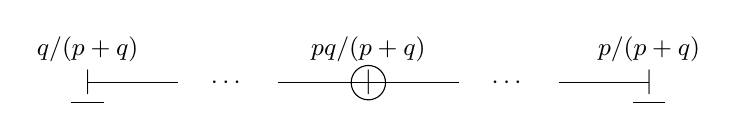
\begin{tikzpicture}[x=1.15cm,y=0.75cm,baseline=(current bounding box.center),every node/.style={font=\small}]
\draw (0,0)--(1,0); \node at (1.55,0) {$\cdots$}; \draw (2.1,0)--(3.1,0); \node[circle,draw,inner sep=1.2pt] at (3.1,0) {$\vert$}; \draw (3.1,0)--(4.1,0); \node at (4.65,0) {$\cdots$}; \draw (5.2,0)--(6.2,0);
\node at (0,0) {$\vert$}; \node at (6.2,0) {$\vert$};
\node[above,yshift=4pt] at (0,0) {$q/(p+q)$}; \node[above,yshift=4pt] at (3.1,0) {$pq/(p+q)$}; \node[above,yshift=4pt] at (6.2,0) {$p/(p+q)$};
\draw (-0.18,-0.34)--(0.18,-0.34); \draw (6.02,-0.34)--(6.38,-0.34);
\end{tikzpicture}
\]

\(B_l\)

\[
\begin{tikzpicture}[x=1.15cm,y=0.75cm,baseline=(current bounding box.center),every node/.style={font=\small}]
\node[circle,draw,inner sep=1.2pt] at (0,0) {$\vert$}; \draw (0,0)--(1,0); \node at (1.7,0) {$\cdots$}; \draw (2.4,0)--(4.2,0); \node at (4.2,0) {$\vert$}; \node at (5.25,0) {$\vert$};
\draw (4.2,0.10)--(5.25,0.10); \draw[->] (4.2,-0.10)--(5.25,-0.10);
\node[above,yshift=4pt] at (0,0) {$1$}; \node[above,yshift=4pt] at (4.2,0) {$1$}; \node[above,yshift=4pt] at (5.25,0) {$1/2$};
\draw (5.07,-0.36)--(5.43,-0.36);
\end{tikzpicture}
\]

\(C_l\)

\[
\begin{tikzpicture}[x=1.15cm,y=0.75cm,baseline=(current bounding box.center),every node/.style={font=\small}]
\node at (0,0) {$\vert$}; \draw (0,0)--(1,0); \node at (1.7,0) {$\cdots$}; \draw (2.4,0)--(4.2,0); \node at (4.2,0) {$\vert$}; \node[circle,draw,inner sep=1.2pt] at (5.25,0) {$\vert$};
\draw[<-] (4.2,0.10)--(5.25,0.10); \draw (4.2,-0.10)--(5.25,-0.10);
\node[above,yshift=4pt] at (0,0) {$1/2$}; \node[above,yshift=4pt] at (5.25,0) {$l/2$};
\draw (-0.18,-0.36)--(0.18,-0.36);
\end{tikzpicture}
\]

\(D_l^{\mathbf R}\)

\[
\begin{tikzpicture}[x=1.15cm,y=0.75cm,baseline=(current bounding box.center),every node/.style={font=\small}]
\node[circle,draw,inner sep=1.2pt] at (0,0) {$\vert$}; \draw (0,0)--(1,0); \node at (1.7,0) {$\cdots$}; \draw (2.4,0)--(4.2,0); \node at (4.2,0) {$\vert$};
\draw (4.2,0)--(5.25,0.65); \draw (4.2,0)--(5.25,-0.65); \node at (5.25,0.65) {$\vert$}; \node at (5.25,-0.65) {$\vert$};
\node[above,yshift=4pt] at (0,0) {$1$}; \node[above,yshift=4pt] at (4.2,0) {$1$}; \node[right,xshift=4pt] at (5.25,0.65) {$1/2$}; \node[right,xshift=4pt] at (5.25,-0.65) {$1/2$};
\draw (5.07,0.29)--(5.43,0.29); \draw (5.07,-1.01)--(5.43,-1.01);
\end{tikzpicture}
\]

\(D_{k+2}^{\mathbf H}\)

\[
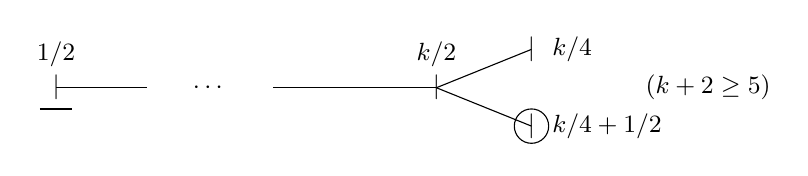
\begin{tikzpicture}[x=1.15cm,y=0.75cm,baseline=(current bounding box.center),every node/.style={font=\small}]
\node at (0,0) {$\vert$}; \draw (0,0)--(1,0); \node at (1.7,0) {$\cdots$}; \draw (2.4,0)--(4.2,0); \node at (4.2,0) {$\vert$};
\draw (4.2,0)--(5.25,0.65); \draw (4.2,0)--(5.25,-0.65); \node at (5.25,0.65) {$\vert$}; \node[circle,draw,inner sep=1.2pt] at (5.25,-0.65) {$\vert$};
\node[above,yshift=4pt] at (0,0) {$1/2$}; \node[above,yshift=4pt] at (4.2,0) {$k/2$}; \node[right,xshift=4pt] at (5.25,0.65) {$k/4$}; \node[right,xshift=4pt] at (5.25,-0.65) {$k/4+1/2$}; \node at (7.2,0) {$(k+2\ge5)$};
\draw (-0.18,-0.36)--(0.18,-0.36);
\end{tikzpicture}
\]

\(E_6\)

\[
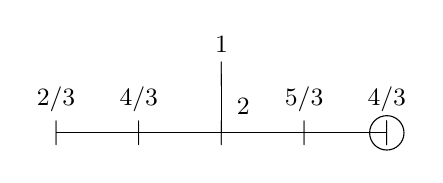
\begin{tikzpicture}[x=1.05cm,y=0.75cm,baseline=(current bounding box.center),every node/.style={font=\small}]
\foreach \x in {0,1,2,3,4}{\node at (\x,0) {$\vert$};} \draw (0,0)--(4,0); \node[circle,draw,inner sep=1.2pt] at (4,0) {$\vert$};
\draw (2,0)--(2,1); \node at (2,1) {$\vert$};
\node[above,yshift=4pt] at (0,0) {$2/3$}; \node[above,yshift=4pt] at (1,0) {$4/3$}; \node[above right,xshift=2pt,yshift=3pt] at (2,0) {$2$}; \node[above,yshift=4pt] at (3,0) {$5/3$}; \node[above,yshift=4pt] at (4,0) {$4/3$}; \node[above,yshift=4pt] at (2,1) {$1$};
\end{tikzpicture}
\]

\(E_7\)

\[
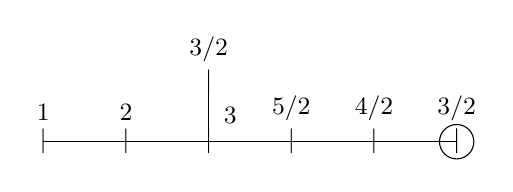
\begin{tikzpicture}[x=1.05cm,y=0.75cm,baseline=(current bounding box.center),every node/.style={font=\small}]
\foreach \x in {0,1,2,3,4,5}{\node at (\x,0) {$\vert$};} \draw (0,0)--(5,0); \node[circle,draw,inner sep=1.2pt] at (5,0) {$\vert$};
\draw (2,0)--(2,1); \node at (2,1) {$\vert$};
\node[above,yshift=4pt] at (0,0) {$1$}; \node[above,yshift=4pt] at (1,0) {$2$}; \node[above right,xshift=2pt,yshift=3pt] at (2,0) {$3$}; \node[above,yshift=4pt] at (3,0) {$5/2$}; \node[above,yshift=4pt] at (4,0) {$4/2$}; \node[above,yshift=4pt] at (5,0) {$3/2$}; \node[above,yshift=4pt] at (2,1) {$3/2$};
\end{tikzpicture}
\]

\SourcePage{16}{262}
\textbf{REMARKS 1.3.10.} (i) For exceptional simple \(G\), no representation \(W\) satisfies 1.3.2.

\begin{enumerate}
\def\labelenumi{(\roman{enumi})}
\setcounter{enumi}{1}
\tightlist
\item
  For classical simple \(G\), except in the case \(D_l^{\mathbf H}\) (\(l\ge5\)), the representations \(W\) of 1.3.2 form a faithful system of representations of \(\widetilde G\). For \(D_l^{\mathbf H}\), one obtains only a faithful representation of a double covering of \(G\) (namely, the algebraic identity component of the automorphism group of a vector space over \(\mathbf H\) equipped with a nondegenerate anti-Hermitian form---an inner form of \(\operatorname{SO}(2n)\)).
\end{enumerate}

\subsection{2. Shimura varieties.}

\subsubsection{2.0. Preliminaries.}

\textbf{2.0.1.} Let \(G\) be a group, let \(\Gamma\) be a subgroup, and let \(\varphi:\Gamma\to\Delta\) be a homomorphism. Suppose that an action \(r\) of \(\Delta\) on \(G\) is given, stabilizing \(\Gamma\), and satisfying

\begin{enumerate}
\def\labelenumi{(\alph{enumi})}
\item
  \(r(\varphi(\gamma))\) is the inner automorphism \(\operatorname{int}_\gamma\) of \(G\);
\item
  \(\varphi\) is compatible with the actions of \(\Delta\), on \(\Gamma\) through \(r\) and on itself through inner automorphisms: \(\varphi(r(\delta)(\gamma))=\operatorname{int}_\delta(\varphi(\gamma))\).
\end{enumerate}

Form the semidirect product \(G\rtimes\Delta\). Conditions (a) and (b) say precisely that the set of elements \(\gamma\cdot\varphi(\gamma)^{-1}\) is a normal subgroup, and we define \(G*_{\Gamma}\Delta\) to be the quotient of \(G\rtimes\Delta\) by this subgroup.

The hypotheses imply that \(Z=\operatorname{Ker}(\varphi)\) is central in \(G\) and that \(\operatorname{Im}(\varphi)\) is a normal subgroup of \(\Delta\). The rows of the diagram

\begin{equation}
\tag{2.0.1.1}
\begin{tikzcd}[column sep=small,row sep=large]
0 \arrow[r] & Z \arrow[r] \arrow[d,equal] & \Gamma \arrow[r] \arrow[d,hook] & \Delta \arrow[r] \arrow[d] & \Delta/\Gamma \arrow[r] \arrow[d,equal] & 0 \\
0 \arrow[r] & Z \arrow[r] & G \arrow[r] & G*_{\Gamma}\Delta \arrow[r] & \Delta/\Gamma \arrow[r] & 0
\end{tikzcd}
\end{equation}

are exact, and hence there is an isomorphism

\[
\Gamma\backslash G\xrightarrow{\sim}\Delta\backslash(G*_{\Gamma}\Delta) \tag{2.0.1.2}
\]

which exhibits a right action of \(G*_{\Gamma}\Delta\) on \(\Gamma\backslash G\). Under this action, \(G\) acts by right translations and \(\Delta\) through the right action \(r^{-1}\).

If \(G\) is a topological group, \(\Delta\) is discrete, and the action \(r\) is continuous, then \(G*_{\Gamma}\Delta\), with the quotient topology induced from \(G\times\Delta\), is a topological group, \(G/\operatorname{Ker}(\varphi)\) is an open subgroup, and (2.0.1.2) is a homeomorphism.

Construction 2.0.1 also makes sense in the category of algebraic groups over a field. If \(G\) is a reductive group over \(k\), there is a canonical isomorphism \(G=\widetilde G*_{Z(\widetilde G)}Z(G)\) (for the trivial action of \(Z(G)\) on \(\widetilde G\)).

\textbf{2.0.2.} Let \(G\) be an algebraic group over a field \(k\), and let \(G^{\mathrm{ad}}\) be the quotient of \(G\) by its center \(Z\). The action of \(G\) on itself by inner automorphisms, \((x,y)\mapsto xyx^{-1}:G\times G\to G\), is invariant under \(Z\times\{e\}\) acting by translation, and therefore factors through an action of \(G^{\mathrm{ad}}\) on \(G\). Notice that the action of \(\gamma\in G^{\mathrm{ad}}(k)\) on \(G(k)\) need not be an inner automorphism of \(G(k)\) (the map from \(G(k)\) to \(G^{\mathrm{ad}}(k)\) is not always surjective). A typical example is the action of \(\operatorname{PGL}(n,k)\) on \(\operatorname{SL}(n,k)\).

Similarly, the ``commutator'' map \((x,y)=xyx^{-1}y^{-1}:G\times G\to G\) is invariant under \(Z\times Z\) acting by translation, and factors through a ``commutator'' map \((\ ,\ ):G^{\mathrm{ad}}\times G^{\mathrm{ad}}\to G\).

\SourcePage{17}{263}
All this, and the fact that these ``commutators'' and ``inner automorphisms'' satisfy the usual identities, is best seen by descent, that is, by interpreting \(G\) as a sheaf of groups on a suitable site and \(G^{\mathrm{ad}}\) as the quotient of this sheaf of groups by its center. In characteristic 0, if one is concerned only with the points of \(G\) over extensions of \(k\), it is enough to use Galois descent---cf.~2.4.1, 2.4.2.

\emph{Variant.} For reductive \(G\) over \(k\), the groups \(G\) and \(\widetilde G\) have the same adjoint group, and the preceding constructions for \(G\) and \(\widetilde G\) are compatible. In particular, the commutator map \((\ ,\ ):G\times G\to G\) has a canonical factorization

\[
(\ ,\ ):G\times G\longrightarrow G^{\mathrm{ad}}\times G^{\mathrm{ad}}\longrightarrow\widetilde G\longrightarrow G.
\]

It follows that the quotient of \(G(k)\) by the normal subgroup \(\rho\widetilde G(k)\) is abelian.

\textbf{2.0.3.} Let \(k\) be a global field of characteristic 0, let \(A\) be its ring of adèles, let \(G\) be a semisimple group over \(k\), and put \(N=\operatorname{Ker}(\rho:\widetilde G\to G)\). Let \(S\) be a finite set of places of \(k\), let \(A_S\) be the ring of \(S\)-adèles (the restricted product over \(v\notin S\)), and put \(\Gamma_S=\rho\widetilde G(A_S)\cap G(k)\) (the intersection being taken in \(G(A_S)\)). This is the group of elements of \(G(k)\) that can be lifted to \(\widetilde G(k_v)\) at every place \(v\notin S\) (recall that \(\rho:\widetilde G(A)\to G(A)\) is proper).

The long exact cohomology sequence identifies \(G(k)/\rho\widetilde G(k)\) with a subgroup of \(H^1(\operatorname{Gal}(\overline k/k),N(\overline k))\), and \(\Gamma_S/\rho\widetilde G(k)\) with the elements of this subgroup that are locally trivial at the places \(v\notin S\). In particular, \(\Gamma_S/\rho\widetilde G(k)\) is contained in the subgroup \(H_*^1(\operatorname{Gal}(\overline k/k),N(\overline k))\) consisting of classes whose restriction to every cyclic subgroup is trivial (argument and notation of {[}12{]}). If \(\operatorname{Im}\operatorname{Gal}(\overline k/k)\) is the image of Galois in \(\operatorname{Aut}N(\overline k)\), then \(H_*^1(\operatorname{Gal}(\overline k/k),N(\overline k))=H_*^1(\operatorname{Im}\operatorname{Gal}(\overline k/k),N(\overline k))\) (loc. cit.); in particular, \(\Gamma_S/\rho\widetilde G(k)\) is finite.

\textbf{PROPOSITION 2.0.4.} \emph{(i) \(\Gamma_S\) depends only on the set of places \(v\in S\) for which the decomposition group \(D_v\subset\operatorname{Im}\operatorname{Gal}(\overline k/k)\) is noncyclic. In particular, it is unchanged if the infinite places are added to \(S\).}

\emph{(ii) \(\Gamma_S/\rho\widetilde G(k)\) is identified with the subgroup of the finite group \(H^1(\operatorname{Im}\operatorname{Gal}(\overline k/k),N(\overline k))\) consisting of classes whose restriction to every decomposition subgroup \(D_v\), \(v\notin S\), is zero. In particular, for sufficiently large \(S\),}

\[
\Gamma_S/\rho\widetilde G(k)=H_*^1(\operatorname{Im}\operatorname{Gal}(\overline k/k),N(\overline k)).
\]

The restriction of an element of \(H_*^1(\operatorname{Im}\operatorname{Gal}(\overline k/k),N(\overline k))\) to a cyclic decomposition group is automatically zero, proving (i). For (ii), we may suppose that \(S\) contains the infinite places. The Hasse principle for \(\widetilde G\) (for classes coming from the center) then ensures that all the elements of the group in (ii) are actually realized as obstruction classes.

\textbf{COROLLARY 2.0.5.} \emph{Every sufficiently small \(S\)-congruence subgroup of \(G(k)\) is contained in \(\Gamma_S\).}

If \(U\) is an \(S\)-congruence subgroup, \(U/(U\cap\rho\widetilde G(k))\) is finite: the obstruction to lifting to \(\widetilde G(k)\) dies in a Galois extension of bounded degree and ramification, and hence belongs to \(H^1(\operatorname{Gal},N(\overline k))\) for a finite quotient \(\operatorname{Gal}\) of \(\operatorname{Gal}(\overline k/k)\). Conditions of \(S\)-congruence then make it possible to pass from this \(H^1\) to \(\Gamma_S/\rho\widetilde G(k)\); cf.~{[}12{]}.

\textbf{REMARK 2.0.6.} We note, moreover, that if \(\widetilde G\) satisfies the strong approxi-

\SourcePage{18}{264}
mation theorem relative to \(S\), every \(S\)-congruence subgroup \(U\subset\Gamma_S\) of \(G(k)\) maps onto \(\Gamma_S/\rho\widetilde G(k)\).

\textbf{COROLLARY 2.0.7.} \emph{For every archimedean place \(v\), every sufficiently small \(S\)-congruence subgroup \(U\) of \(G(k)\) is contained in the topological identity component \(G(k_v)^+\) of \(G(k_v)\).}

Since \(\widetilde G(k_v)\) is connected, \(G(k_v)^+=\rho\widetilde G(k_v)\), and \(U\subset\Gamma_S=\Gamma_{S\cup\{v\}}\subset G(k_v)^+\) (2.0.4 and 2.0.5).

\textbf{COROLLARY 2.0.8.} \emph{The subgroup \(G(k)\rho\widetilde G(A_S)\) of \(G(A_S)\) is closed and is topologically isomorphic to \(\rho\widetilde G(A_S)*_{\Gamma_S}G(k)\) (that is, \(\rho\widetilde G(A_S)\) is an open subgroup).}

It is a subgroup because, by 2.0.2, \(\rho\widetilde G(A_S)\) is normal in \(G(A_S)\) with commutative quotient. Let \(T\supset S\) be large enough that \(\widetilde G(k)\) is dense in \(\widetilde G(A_T)\) (strong approximation). Write \(k_{T-S}\) for the product of the \(k_v\) for \(v\in T-S\). For a compact open subgroup \(K\) of \(G(A_T)\), we have

\[
G(k)\rho\widetilde G(A_S)
=G(k)\rho\bigl(\widetilde G(k)\cdot\widetilde G(k_{T-S})\times\rho^{-1}K\bigr)
\subset G(k)\bigl(\rho\widetilde G(k_{T-S})\times K\bigr).
\]

By 2.0.5, when \(K\) is sufficiently small we have, in \(G(A_T)\), \(G(k)\cap K\subset\Gamma_T\); hence, in \(G(A_S)\), \(G(k)\cap(\rho\widetilde G(k_{T-S})\times K)\subset\Gamma_S\subset\rho\widetilde G(A_S)\). The intersection of \(G(k)\rho\widetilde G(A_S)\) with the open subgroup \(\rho\widetilde G(k_{T-S})\times K\) is therefore contained in \(\rho\widetilde G(A_S)\), and the corollary follows.

\textbf{COROLLARY 2.0.9.} \emph{If \(\widetilde G\) satisfies the strong approximation theorem relative to \(S\), the closure of \(G(k)\) in \(G(A_S)\) is \(G(k)\cdot\rho\widetilde G(A_S)\).}

\textbf{2.0.10.} Let \(T\) be a torus over \(k\), and let \(S\) be a finite set of places containing the archimedean places. Let \(U\subset T(k)\) be the group of \(S\)-units. By a theorem of Chevalley, every finite-index subgroup of \(U\) is a congruence subgroup (see {[}12{]} for an elegant proof). It follows that, if \(T'\to T\) is an isogeny, the image of a congruence subgroup for \(T'\) is a congruence subgroup for \(T\).

\textbf{2.0.11.} Let \(G\) be reductive over \(k\), let \(\rho:\widetilde G\to G^{\mathrm{der}}\) be the universal covering of its derived group, and let \(Z^0\) be the identity component of its center \(Z\). Here are some consequences of 2.0.10 (the finite set \(S\) of places is assumed to contain the archimedean places).

\textbf{COROLLARY 2.0.12.} \emph{For every finite-index subgroup \(U\) of the group of \(S\)-units of \(Z(k)\), there exists a compact open subgroup \(K\) of \(G(A_S)\) such that}

\[
G(k)\cap\bigl(K\cdot G^{\mathrm{der}}(A_S)\bigr)\subset G^{\mathrm{der}}(k)\cdot U.
\]

Apply 2.0.10 to the isogeny \(Z^0\to G/G^{\mathrm{der}}\). If \(K\) is small, an element \(\gamma\in G(k)\) lying in \(K\cdot G^{\mathrm{der}}(A_S)\) has a small image in \((G/G^{\mathrm{der}})(k)\) for the topology of \(S\)-congruence subgroups, so this image can be lifted to a small element \(z\in Z(k)\), and \(\gamma=(\gamma z^{-1})\cdot z\).

\textbf{COROLLARY 2.0.13.} \emph{The product of a congruence subgroup of \(G^{\mathrm{der}}\) and a finite-index subgroup of the group of \(S\)-units of \(Z^0(k)\) is an \(S\)-congruence subgroup of \(G(k)\).}

\SourcePage{19}{265}
\textbf{COROLLARY 2.0.14.} \emph{Every sufficiently small \(S\)-congruence subgroup of \(G(k)\) is contained in the topological identity component \(G(\mathbf R)^+\) of \(G(\mathbf R)\).}

Apply 2.0.13, 2.0.7 to \(G^{\mathrm{der}}\), and 2.0.10 to \(Z^0\).

\textbf{2.0.15.} We know that \(G^{\mathrm{der}}(k)\rho\widetilde G(A)\) is open in \(G(k)\rho\widetilde G(A)\) (since it is the inverse image of \(\{e\}\subset (G/G^{\mathrm{der}})(k)\), the discrete subgroup of \((G/G^{\mathrm{der}})(A)\)). By 2.0.8, \(G(k)\rho\widetilde G(A)\) is therefore a closed subgroup of \(G(A)\). Put

\[
\pi(G)=G(A)/G(k)\rho\widetilde G(A). \tag{2.0.15.1}
\]

The existence of commutators in 2.0.2 shows that the action of \(G^{\mathrm{ad}}(k)\) on \(\pi(G)\), induced by the action of \(G^{\mathrm{ad}}\) on \(G\) in 2.0.2, is trivial.

\subsubsection{2.1. Shimura varieties.}

\textbf{2.1.1.} Let \(G\) be a reductive group defined over \(\mathbf Q\), and let \(X\) be a \(G(\mathbf R)\)-conjugacy class of morphisms of real algebraic groups from \(S\) to \(G_{\mathbf R}\). We assume that the following axioms hold (the notation is that of 1.1.1 and 1.1.11):

(2.1.1.1) For \(h\in X\), \(\operatorname{Lie}(G_{\mathbf R})\) is of type \(\{(-1,1),(0,0),(1,-1)\}\).

(2.1.1.2) The involution \(\operatorname{int}h(i)\) is a Cartan involution of the adjoint group \(G_{\mathbf R}^{\mathrm{ad}}\).

(2.1.1.3) The adjoint group has no factor \(G'\) defined over \(\mathbf Q\) on which the projection of \(h\) is trivial.

Axiom 2.1.1 ensures that the morphism \(w_h\) (\(h\in X\)) takes values in the center of \(G\) and is therefore independent of \(h\). We denote it by \(w_X\), or simply by \(w\). Some simplifications occur when one assumes that:

(2.1.1.4) The morphism \(w:G_m\to G_{\mathbf R}\) is defined over \(\mathbf Q\).

(2.1.1.5) \(\operatorname{int}h(i)\) is a Cartan involution of the group \((G/w(G_m))_{\mathbf R}\).

By 1.1.14(i), \(X\) has a unique complex structure such that, for every representation \(V\) of \(G_{\mathbf R}\), the Hodge filtration \(F_h\) of \(V\) varies holomorphically with \(h\). For this complex structure, the connected components of \(X\) are Hermitian symmetric domains. The proof of 1.1.17 also shows that, if \(G_{\mathbf R}^{\mathrm{ad}}\) is decomposed into simple factors, \(h\) projects trivially onto the compact factors, and every connected component of \(X\) is the product of the Hermitian symmetric spaces corresponding to the noncompact factors. Axiom 2.1.1.3 may also be expressed by saying that \(G^{\mathrm{ad}}\) (or, equivalently, \(\widetilde G\)) has no factor \(G'\) defined over \(\mathbf Q\) such that \(G'(\mathbf R)\) is compact; the strong approximation theorem then ensures that \(\widetilde G(\mathbf Q)\) is dense in \(\widetilde G(A^f)\).

\textbf{2.1.2.} The \emph{Shimura varieties} \({}_K M_{\mathbf C}(G,X)\)---or simply \({}_K M_{\mathbf C}\)---are the quotients

\[
{}_K M_{\mathbf C}(G,X)=G(\mathbf Q)\backslash X\times(G(A^f)/K)
\]

for \(K\) a compact open subgroup of \(G(A^f)\). By 1.2.7, and with the notation of 0.3, the action of \(G(\mathbf R)\) on \(X\) makes \(\pi_0(X)\) a principal homogeneous space under \(G(\mathbf R)/G(\mathbf R)_+\). Since \(G(\mathbf Q)\) is dense in \(G(\mathbf R)\) (the real approximation theorem), we have \(G(\mathbf Q)/G(\mathbf Q)_+\xrightarrow{\sim}G(\mathbf R)/G(\mathbf R)_+\); hence, if \(X^+\) is a connected component of \(X\),

\[
{}_K M_{\mathbf C}(G,X)=G(\mathbf Q)_+\backslash X^+\times(G(A^f)/K).
\]

This quotient is the disjoint union, indexed by the finite double-coset set \(G(\mathbf Q)_+\backslash G(A^f)/K\), of the quotients \(\Gamma_g\backslash X^+\) of the Hermitian symmetric domain \(X^+\) by the images \(\Gamma_g\subset G^{\mathrm{ad}}(\mathbf R)^+\) of the subgroups \(\Gamma'_g=gKg^{-1}\cap G(\mathbf Q)_+\) of \(G(\mathbf Q)_+\). The \(\Gamma_g\) are arithmetic groups, and consequently \(\Gamma_g\backslash X^+\) has the structure of an analytic space.

\SourcePage{20}{266}
Article {[}2{]} supplies a natural quasi-projective algebraic-variety structure on these quotients, and therefore on \({}_K M_{\mathbf C}(G,X)\). If \(\Gamma_g\) is torsion-free (as is the case when \(K\) is sufficiently small), it follows from {[}3{]} that this structure is unique. More precisely, for every reduced scheme \(Z\), an analytic morphism from \(Z\) to \(\Gamma_g\backslash X^+\) is automatically algebraic.

\textbf{2.1.3.} We have

\[
\pi_0{}_K M_{\mathbf C}
=G(\mathbf Q)\backslash\pi_0(X)\times(G(A^f)/K)
=G(\mathbf Q)\backslash G(A)/(G(\mathbf R)_+\times K)
=G(\mathbf Q)_+\backslash G(A^f)/K.
\]

Since \(G(A^f)/K\) is discrete, \(G(\mathbf Q)_+\) may be replaced by its closure in \(G(A^f)\). The connectedness of \(\widetilde G(\mathbf R)\) ensures that \(\rho\widetilde G(\mathbf Q)\subset G(\mathbf Q)_+\). By the strong approximation theorem for \(\widetilde G\), \(\rho\widetilde G(\mathbf Q)\) is dense in \(\rho\widetilde G(A^f)\), and \(G(\mathbf Q)_+^{-}\supset\rho\widetilde G(A^f)\). Hence

\[
\tag{2.1.3.1}
\begin{aligned}
\pi_0{}_K M_{\mathbf C}
&=G(\mathbf Q)_+\rho\widetilde G(A^f)\backslash G(A^f)/K\\
&=G(A^f)/\rho\widetilde G(A^f)\cdot G(\mathbf Q)_+\cdot K
 =G(A^f)/(G(\mathbf Q)_+^{-}\cdot K),
\end{aligned}
\]

because \(\rho\widetilde G(A^f)\) is a normal subgroup with abelian quotient. Likewise, putting \(\bar\pi_0\pi(G)=\pi_0\pi(G)/\pi_0G(\mathbf R)_+\), we have

\[
\tag{2.1.3.2}
\begin{aligned}
\pi_0{}_K M_{\mathbf C}
&=G(A)/(\rho\widetilde G(A)\cdot G(\mathbf Q)\cdot G(\mathbf R)_+\times K)\\
&=\pi(G)/(G(\mathbf R)_+\times K)
 =\bar\pi_0\pi(G)/K.
\end{aligned}
\]

In particular, \(\pi_0{}_K M_{\mathbf C}\) depends only on the image of \(K\) in \(G(A)/\rho\widetilde G(A)\).

\textbf{2.1.4.} As \(K\) varies (and becomes progressively smaller), the \({}_K M_{\mathbf C}\) form a projective system. It carries a right action of \(G(A^f)\): a system of isomorphisms

\[
g:{}_K M_{\mathbf C}\xrightarrow{\sim}{}_{g^{-1}Kg}M_{\mathbf C}.
\]

It is convenient instead to consider the scheme \(M_{\mathbf C}(G,X)\)---or simply \(M_{\mathbf C}\)---which is the projective limit of the \({}_K M_{\mathbf C}\). The projective limit exists because the transition morphisms are finite. This scheme carries a right action of \(G(A^f)\) and recovers the \({}_K M_{\mathbf C}\): \({}_K M_{\mathbf C}=M_{\mathbf C}/K\).

We shall determine \(M_{\mathbf C}\) and its decomposition into connected components.

\textbf{DEFINITION 2.1.5.} \emph{Fix a connected component \(X^+\) of \(X\). The neutral component \(M_{\mathbf C}^0\) of \(M_{\mathbf C}\) is the connected component containing the image of \(X^+\times\{e\}\subset X\times G(A^f)\).}

\textbf{DEFINITION 2.1.6.} \emph{Let \(G_0\) be an adjoint group over \(\mathbf Q\) with no factor \(G'_0\) defined over \(\mathbf Q\) such that \(G'_0(\mathbf R)\) is compact, and let \(G_1\) be a covering of \(G_0\). The topology \(\tau(G_1)\) on \(G_0(\mathbf Q)\) is the topology for which the images of the congruence subgroups of \(G_1(\mathbf Q)\) form a fundamental system of neighborhoods of the identity.}

We shall denote completion for this topology by \(^{\wedge}(\mathrm{rel.}\,G_1)\), or simply by \(^{\wedge}\). Let \(\rho:\widetilde G_0\to G_1\) be the natural map, let \(^{-}\) denote closure in \(G_1(A^f)\), and put \(\Gamma=\rho\widetilde G_0(A)\cap G_1(\mathbf Q)\). Since \(\widetilde G_0(\mathbf R)\) is connected, \(\Gamma\subset G_1(\mathbf Q)^+\). We have (2.0.9, 2.0.14)

\[
G_0(\mathbf Q)^{\wedge}(\mathrm{rel.}\,G_1)
=G_1(\mathbf Q)^{-}*_{G_1(\mathbf Q)}G_0(\mathbf Q)
=\rho\widetilde G_0(A^f)*_{\Gamma}G_0(\mathbf Q),
\tag{2.1.6.1}
\]

\[
G_0(\mathbf Q)^{+\wedge}(\mathrm{rel.}\,G_1)
=G_1(\mathbf Q)_+^{-}*_{G_1(\mathbf Q)_+}G_0(\mathbf Q)^+
=\rho\widetilde G_0(A^f)*_{\Gamma}G_0(\mathbf Q)^+.
\tag{2.1.6.2}
\]

\textbf{PROPOSITION 2.1.7.} \emph{The neutral component \(M_{\mathbf C}^0\) is the projective limit of the quotients \(\Gamma\backslash X^+\), where \(\Gamma\) runs through the arithmetic subgroups of \(G^{\mathrm{ad}}(\mathbf Q)^+\) that are open for the topology \(\tau(G^{\mathrm{der}})\).}

\SourcePage{21}{267}
By 2.1.2, this is the limit of the \(\Gamma\backslash X^0\), where \(\Gamma\) is the image of a congruence subgroup of \(G(\mathbf Q)_+\). Corollary 2.0.13 allows \(G\) to be replaced by \(G^{\mathrm{der}}\).

\textbf{2.1.8.} The projection from \(G\) to \(G^{\mathrm{ad}}\) induces an isomorphism from \(X^+\) onto a \(G(\mathbf R)^+\)-conjugacy class of morphisms from \(S\) to \(G_{\mathbf R}^{\mathrm{ad}}\); by 2.1.7, \(M_{\mathbf C}^0(G,X)\) depends only on \(G^{\mathrm{ad}}\), \(G^{\mathrm{der}}\), and this class. Let us formalize this observation. Let \(G\) be an adjoint group, let \(X^+\) be a \(G(\mathbf R)^+\)-conjugacy class of morphisms from \(S\) to \(G(\mathbf R)\) satisfying (2.1.1), (2.1.2), and (2.1.3), and let \(G_1\) be a covering of \(G\). The \emph{connected Shimura varieties} (relative to \(G,G_1,X^+\)) are the quotients \(\Gamma\backslash X^+\), where \(\Gamma\) is an arithmetic subgroup of \(G(\mathbf Q)^+\) open for the topology \(\tau(G_1)\). We denote by \(M_{\mathbf C}^0(G,G_1,X^+)\) their projective limit as \(\Gamma\) becomes progressively smaller. The action by transport of structure of \(G(\mathbf Q)^+\) on \(M_{\mathbf C}^0(G,G_1,X^+)\) extends continuously to an action of the completion \(G(\mathbf Q)^{+\wedge}(\mathrm{rel.}\,G_1)\).

With the notation of 2.1.7 and the above identification of \(X^+\) with a \(G(\mathbf R)^+\)-conjugacy class of morphisms from \(S\) to \(G_{\mathbf R}^{\mathrm{ad}}\), we have

\[
M_{\mathbf C}^0(G,X)=M_{\mathbf C}^0(G^{\mathrm{ad}},G^{\mathrm{der}},X^+).
\]

\textbf{2.1.9.} Let \(Z\) be the center of \(G\), and let \(Z(\mathbf Q)^{-}\) be the closure of \(Z(\mathbf Q)\) in \(Z(A^f)\). By Chevalley (2.0.10), this is the completion of \(Z(\mathbf Q)\) for the topology of finite-index subgroups of the unit group; it receives isomorphically the closure of \(Z(\mathbf Q)\) in \(\pi_0Z(\mathbf R)\times Z(A^f)\).

For a compact open subgroup \(K\subset G(A^f)\), we have \(Z(\mathbf Q)\cdot K=Z(\mathbf Q)^{-}\cdot K\) (in \(Z(A^f)\)), and

\[
\begin{aligned}
{}_K M_{\mathbf C}
&=G(\mathbf Q)\backslash X\times(G(A^f)/K)\\
&=\frac{G(\mathbf Q)}{Z(\mathbf Q)}\backslash X\times\bigl(G(A^f)/(Z(\mathbf Q)\cdot K)\bigr)\\
&=\frac{G(\mathbf Q)}{Z(\mathbf Q)}\backslash X\times\bigl(G(A^f)/(Z(\mathbf Q)^{-}\cdot K)\bigr).
\end{aligned}
\]

The action of \(G(\mathbf Q)/Z(\mathbf Q)\) on \(X\times(G(A^f)/Z(\mathbf Q)^{-})\) is proper. This permits passage to the limit over \(K\):

\textbf{PROPOSITION 2.1.10.} \emph{We have}

\[
M_{\mathbf C}(G,X)=\frac{G(\mathbf Q)}{Z(\mathbf Q)}\backslash X\times\bigl(G(A^f)/Z(\mathbf Q)^{-}\bigr).
\]

\textbf{COROLLARY 2.1.11.} \emph{If conditions 2.1.4 and 2.1.5 hold, then \(M_{\mathbf C}(G,X)=G(\mathbf Q)\backslash X\times G(A^f)\).}

In this case, \(Z(\mathbf Q)\) is discrete in \(Z(A^f)\) and \(Z(\mathbf Q)^{-}=Z(\mathbf Q)\).

\textbf{COROLLARY 2.1.12.} \emph{The right action of \(G(A^f)\) factors through \(G(A^f)/Z(\mathbf Q)^{-}\).}

\textbf{2.1.13.} Let \(G^{\mathrm{ad}}(\mathbf R)_1\) be the image of \(G(\mathbf R)\) in \(G^{\mathrm{ad}}(\mathbf R)\), and let \(G^{\mathrm{ad}}(\mathbf Q)_1=G^{\mathrm{ad}}(\mathbf Q)\cap G^{\mathrm{ad}}(\mathbf R)_1\). The action of \(G^{\mathrm{ad}}\) on \(G\) from 2.0.2 induces a left action of \(G^{\mathrm{ad}}(\mathbf Q)_1\) on the system of the \({}_K M_{\mathbf C}\),

\[
\operatorname{int}(\gamma):{}_K M_{\mathbf C}\xrightarrow{\sim}{}_{\gamma K\gamma^{-1}}M_{\mathbf C},
\]

and hence on the limit \(M_{\mathbf C}\). For \(\gamma\in G^{\mathrm{ad}}(\mathbf Q)^+\), this action stabilizes the neutral component (and therefore all components; see below) and induces on it the action of 2.1.6.

Convert this action into a right action, denoted \(\cdot\gamma\). If \(\gamma\) is the image of

\SourcePage{22}{268}
\(\delta\in G(\mathbf Q)\), the action \(\cdot\gamma\) coincides with the action of \(\delta\) viewed as an element of \(G(A^f)\): if \(u\in M_{\mathbf C}\) is the image of \((x,g)\in X\times G(A^f)\), then \(u\cdot\gamma\) is the image of

\[
(\gamma^{-1}(x),\operatorname{int}_{\gamma}^{-1}(g))
=(\delta^{-1}(x),\delta^{-1}g\delta)
\sim(x,g\delta)\pmod{G(\mathbf Q)}\quad\text{on the left}.
\]

Thus we obtain a right action on \(M_{\mathbf C}\) of the group

\[
\frac{G(A^f)}{Z(\mathbf Q)^{-}}*_{G(\mathbf Q)/Z(\mathbf Q)}G^{\mathrm{ad}}(\mathbf Q)_1
=\frac{G(A^f)}{Z(\mathbf Q)^{-}}*_{G(\mathbf Q)_+/Z(\mathbf Q)}G^{\mathrm{ad}}(\mathbf Q)^+.
\tag{2.1.13.1}
\]

\textbf{PROPOSITION 2.1.14.} \emph{The right action of \(G(A^f)\) on \(\pi_0M_{\mathbf C}\) makes \(\pi_0M_{\mathbf C}\) a principal homogeneous space under its abelian quotient \(G(A^f)/G(\mathbf Q)_+^{-}=\bar\pi_0\pi(G)\).}

This follows immediately by passing to the limit in the formulas of 2.1.3.

\textbf{2.1.15.} Since \(G^{\mathrm{ad}}(\mathbf Q)\) acts trivially on \(\pi(G)\) (2.0.15), and \(G^{\mathrm{ad}}(\mathbf Q)^+\) stabilizes at least one connected component (2.1.13), the group \(G^{\mathrm{ad}}(\mathbf Q)^+\) stabilizes all of them. For the action of the group (2.1.13.1) on \(M_{\mathbf C}\) described in 2.1.13, the stabilizer of each connected component is therefore

\[
\frac{G(\mathbf Q)_+^{-}}{Z(\mathbf Q)^{-}}*_{G(\mathbf Q)_+/Z(\mathbf Q)}G^{\mathrm{ad}}(\mathbf Q)^+
\underset{2.0.13}{=}G^{\mathrm{ad}}(\mathbf Q)^{+\wedge}(\mathrm{rel.}\,G^{\mathrm{der}}).
\tag{2.1.15.1}
\]

\textbf{Summary 2.1.16.} \emph{The group \(G(A^f)/Z(\mathbf Q)^{-}*_{G(\mathbf Q)/Z(\mathbf Q)}G^{\mathrm{ad}}(\mathbf Q)_1\) acts on the right on \(M_{\mathbf C}\). The profinite set \(\pi_0M_{\mathbf C}\) is a principal homogeneous space under the action of the abelian quotient \(G(A^f)/G(\mathbf Q)_+^{-}=\bar\pi_0\pi(G)\) of this group by the closure of \(G^{\mathrm{ad}}(\mathbf Q)^+\). This closure is the completion of \(G^{\mathrm{ad}}(\mathbf Q)^+\) for the topology of the images of the congruence subgroups of \(G^{\mathrm{der}}(\mathbf Q)\). After its action on the neutral component is converted into a left action, it is the action of 2.1.8.}

\subsubsection{2.2. Canonical models.}

\textbf{2.2.1.} Let \(G\) and \(X\) be as in 2.1.1. For \(h\in X\), the morphism \(\mu_h\) (1.1.1, supplemented by 1.1.11) is a morphism over \(\mathbf C\) of algebraic groups defined over \(\mathbf Q\):

\[
\mu_h:G_m\to G_{\mathbf C}.
\]

The \emph{reflex field} \(E(G,X)\subset\mathbf C\) of \((G,X)\) is the field of definition of its conjugacy class. If \(X^+\) is a connected component of \(X\), it will sometimes be denoted by \(E(G,X^+)\).

Let \((G',X')\) and \((G'',X'')\) be as in 2.1.1. If a morphism \(f:G'\to G''\) sends \(X'\) into \(X''\), then \(E(G',X')\supset E(G'',X'')\).

\textbf{2.2.2.} Let \(T\) be a torus, let \(E\) be a number field, and let \(\mu\) be a morphism, defined over \(E\), from \(G_m\) into \(T_E\). The group \(E^*\), viewed as an algebraic group over \(\mathbf Q\), is the Weil restriction of scalars \(R_{E/\mathbf Q}(G_m)\). Applying \(R_{E/\mathbf Q}\) to \(\mu\) gives \(R_{E/\mathbf Q}(\mu)\):

\[
E^*\to R_{E/\mathbf Q}T_E.
\]

There is also the norm morphism \(N_{E/\mathbf Q}:R_{E/\mathbf Q}T_E\to T\) (on rational points it is the norm \(T(E)\to T(\mathbf Q)\)). Composition therefore gives a morphism

\[
N_{E/\mathbf Q}\circ R_{E/\mathbf Q}(\mu):E^*\to T.
\]

We shall denote it simply by \(NR_E(\mu)\), or even by \(NR(\mu)\). If \(E'\) is an extension of \(E\), then \(\mu\) is still defined over \(E'\), and

\[
NR_{E'}(\mu)=NR_E(\mu)\circ N_{E'/E}. \tag{2.2.2.1}
\]

\textbf{2.2.3.} In particular, let \(T\) be a torus, let \(h:S\to T_{\mathbf R}\), and let \(X=\{h\}\). If \(E\subset\mathbf C\) contains \(E(T,X)\), then \(\mu_h\) is defined over \(E\), giving a morphism \(NR(\mu_h):E^*\to T\). Passing to adelic points modulo rational points yields a homomorphism from the idèle class group \(C(E)\) of \(E\) to \(T(\mathbf Q)\backslash T(A)\), and passing to sets of connected components gives a morphism

\SourcePage{23}{269}
\[
\pi_0NR(\mu_h):\pi_0C(E)\to\pi_0\bigl(T(\mathbf Q)\backslash T(A)\bigr).
\]

Global class field theory identifies \(\pi_0C(E)\) with the abelianized Galois group of \(E\).

The group \(\pi_0(T(\mathbf Q)\backslash T(A))\) is a profinite group, the projective limit of the finite groups \(T(\mathbf Q)\backslash T(A)/(T(\mathbf R)^+\times K)\) for compact open \(K\subset T(A^f)\). It is \(\pi_0T(\mathbf R)\times T(A^f)/T(\mathbf Q)^{-}\). The Shimura varieties \({}_K M_{\mathbf C}(T,X)\) are the finite sets

\[
T(\mathbf Q)\backslash\{h\}\times T(A^f)/K=T(\mathbf Q)\backslash T(A^f)/K.
\]

Their projective limit \(T(A^f)/T(\mathbf Q)^{-}\), calculated in 2.1.10, is the quotient of \(\pi_0(T(\mathbf Q)\backslash T(A))\) by \(\pi_0T(\mathbf R)\).

We call the morphism

\[
r_E(T,X):\operatorname{Gal}(\overline{\mathbf Q}/E)^{\mathrm{ab}}\to T(A^f)/T(\mathbf Q)^{-}
\]

the \emph{reciprocity morphism}. It is the inverse of the composite of the isomorphism of global class field theory (0.8), \(\pi_0NR(\mu_h)\), and the projection from \(\pi_0T(A)/T(\mathbf Q)\) onto \(T(A^f)/T(\mathbf Q)^{-}\). It defines an action \(r_E\) of \(\operatorname{Gal}(\overline{\mathbf Q}/E)^{\mathrm{ab}}\) on the \({}_K M_{\mathbf C}(T,X)\): \(\sigma\) acts by right translation by \(r_E(T,X)(\sigma)\).

The universal case (with respect to \(E\)) is \(E=E(T,X)\). It follows from (2.2.2.1) that the action \(r_E\) of \(\operatorname{Gal}(\overline{\mathbf Q}/E)\) is the restriction to \(\operatorname{Gal}(\overline{\mathbf Q}/E)\subset\operatorname{Gal}(\overline{\mathbf Q}/E(T,X))\) of \(r_{E(T,X)}\).

\textbf{2.2.4.} Let \(G\) and \(X\) be as in 2.1.1. A point \(h\in X\) is called \emph{special}, or of \emph{CM type}, if \(h:S\to G(\mathbf R)\) factors through a torus \(T\subset G\) defined over \(\mathbf Q\). If \(T\) is such a torus, the Cartan involution \(\operatorname{int}h(i)\) is trivial on the image of \(T(\mathbf R)\) in the adjoint group, and that image is therefore compact. The field \(E(T,\{h\})\) depends only on \(h\). It is the \emph{reflex field} \(E(h)\) of \(h\).

We transfer this terminology to points of \({}_K M_{\mathbf C}(G,X)\) and \(M_{\mathbf C}(G,X)\). If \(x\in{}_K M_{\mathbf C}(G,X)\) (respectively, \(M_{\mathbf C}(G,X)\)) is the class of \((h,g)\in X\times G(A^f)\), then the \(G(\mathbf Q)\)-conjugacy class of \(h\) depends only on \(x\). We say that \(x\) is special if \(h\) is special, that \(E(h)\) is the reflex field \(E(x)\) of \(x\), and that the \(G(\mathbf Q)\)-conjugacy class of \(h\) is the \emph{type} of \(x\).

On the set of special points of \({}_K M_{\mathbf C}(G,X)\) (respectively, \(M_{\mathbf C}(G,X)\)) of a fixed type, corresponding to a reflex field \(E\), we now define an action \(r\) of \(\operatorname{Gal}(\overline{\mathbf Q}/E)\). Let \(x\in{}_K M_{\mathbf C}(G,X)\) (respectively, \(M_{\mathbf C}(G,X)\)) be the class of \((h,g)\in X\times G(A^f)\); let \(T\subset G\) be a torus defined over \(\mathbf Q\) through which \(h\) factors; let \(\sigma\in\operatorname{Gal}(\overline{\mathbf Q}/E)\); and let \(\widetilde r(\sigma)\) be a representative in \(T(A^f)\) of \(r_E(T,\{h\})(\sigma)\in T(A^f)/T(\mathbf Q)^{-}\). Define \(r(\sigma)x\) to be the class of \((h,\widetilde r(\sigma)g)\). The reader will check that this class depends only on \(x\) and \(\sigma\). The action so defined commutes with the right action of \(G(A^f)\) on \(M_{\mathbf C}(G,X)\).

\textbf{2.2.5.} A \emph{canonical model} \(M(G,X)\) of \(M_{\mathbf C}(G,X)\) is a form of \(M_{\mathbf C}(G,X)\) over \(E(G,X)\), equipped with the right action of \(G(A^f)\), such that

\begin{enumerate}
\def\labelenumi{(\alph{enumi})}
\item
  the special points are algebraic;
\item
  on the set of special points of a fixed type \(\tau\), corresponding to a reflex field \(E(\tau)\), the Galois group \(\operatorname{Gal}(\overline{\mathbf Q}/E(\tau))\subset\operatorname{Gal}(\overline{\mathbf Q}/E(G,X))\) acts by the action of 2.2.4.
\end{enumerate}

By a ``form'' we mean a scheme \(M\) over \(E(G,X)\), equipped with a right action of \(G(A^f)\) and an equivariant isomorphism

\[
M\otimes_{E(G,X)}\mathbf C\xrightarrow{\sim}M_{\mathbf C}(G,X).
\]

Let \(E\subset\mathbf C\) be a number field containing \(E(G,X)\). A \emph{weakly canonical model} of \(M_{\mathbf C}(G,X)\) over \(E\) is a form of \(M_{\mathbf C}(G,X)\) over \(E\), equipped with the right action of \(G(A^f)\), satisfying (a) and

(b*) the same condition as (b), with \(\operatorname{Gal}(\overline{\mathbf Q}/E(\tau))\) replaced by \(\operatorname{Gal}(\overline{\mathbf Q}/E(\tau))\cap\operatorname{Gal}(\overline{\mathbf Q}/E)\).

\textbf{2.2.6.} In {[}5, 5.4, 5.5{]}, drawing on Shimura's methods, we have

\SourcePage{24}{270}
shown that \(M_{\mathbf C}(G,X)\) has at most one weakly canonical model over \(E\) (for \(E(G,X)\subset E\subset\mathbf C\)), and that, when it exists, it is functorial in \((G,X)\).

\subsubsection{2.3. Construction of canonical models.}

In this section we determine cases in which the following criterion, proved in {[}5, 4.21, 5.7{]}, applies to construct canonical models.

\textbf{Criterion 2.3.1.} \emph{Let \((G,X)\) be as in 2.1.1, let \(V\) be a rational vector space equipped with a nondegenerate alternating form \(\Psi\), and let \(\mathfrak S^{\pm}\) be the corresponding double Siegel half-space (cf.~1.3.1). If there exists an embedding \(G\hookrightarrow\operatorname{CSp}(V)\) sending \(X\) into \(\mathfrak S^{\pm}\), then \(M_{\mathbf C}(G,X)\) has a canonical model \(M(G,X)\).}

\textbf{PROPOSITION 2.3.2.} \emph{Let \((G,X)\) be as in 2.1.1, let \(w=w_h\) (\(h\in X\)), and let \((V,\rho)\) be a faithful representation of \(G\) of type \(\{(-1,0),(0,-1)\}\). If \(\operatorname{int}h(i)\) is a Cartan involution of \(G_{\mathbf R}/w(G_m)\), there is an alternating form \(\Psi\) on \(V\) such that \(\rho\) induces \((G,X)\hookrightarrow(\operatorname{CSp}(V),\mathfrak S^{\pm})\).}

By hypothesis, the faithful representation \(V\) is homogeneous of weight \(-1\). Thus the weight \(w\) is defined over \(\mathbf Q\), and we take for \(\Psi\) a polarization form as in 1.1.18(b).

\textbf{COROLLARY 2.3.3.} \emph{Let \((G,X)\) be as in 2.1.1, let \(w=w_h\) (\(h\in X\)), and let \((V,\rho)\) be a faithful representation of \(G\) of type \(\{(-1,0),(0,-1)\}\). If the center \(Z^0\) of \(G\) splits over a field of CM type, then there exists a subgroup \(G_2\) of \(G\), with the same derived group and through which \(X\) factors, and an alternating form \(\Psi\) on \(V\), such that \(\rho\) induces \((G_2,X)\hookrightarrow(\operatorname{CSp}(V),\mathfrak S^{\pm})\).}

The hypothesis on \(Z^0\) says that the largest compact subtorus of \(Z_{\mathbf R}^0\) is defined over \(\mathbf Q\). Take \(G_2\) to be generated by the derived group, this torus, and the image of \(w\), and apply 2.3.2.

\textbf{2.3.4.} Let \((G,X)\) be as in 2.1.1, with \(G\) adjoint and \(\mathbf Q\)-simple. Axiom (2.1.1.2) ensures that \(G_{\mathbf R}\) is an inner form of its compact form. We exploit this fact.

\begin{enumerate}
\def\labelenumi{(\alph{enumi})}
\item
  The simple components of \(G_{\mathbf R}\) are absolutely simple. If \(G\) is written as obtained by Weil restriction of scalars, \(G=R_{F/\mathbf Q}G^s\), with \(G^s\) absolutely simple over \(F\), this means that \(F\) is totally real. Put \(I\) for the set of real embeddings of \(F\) and, for \(v\in I\), put \(G_v=G^s\otimes_{F,v}\mathbf R\) and let \(D_v\) be the Dynkin diagram of \(G_{v\mathbf C}\). We have \(G_{\mathbf R}=\prod G_v\) and \(G_{\mathbf C}=\prod G_{v\mathbf C}\), and the Dynkin diagram \(D\) of \(G_{\mathbf C}\) is the disjoint union of the \(D_v\). The Galois group \(\operatorname{Gal}(\overline{\mathbf Q}/\mathbf Q)\) acts on \(D\) and \(I\) compatibly with the projection from \(D\) to \(I\).
\item
  Complex conjugation acts on \(D\) by the opposition involution. This involution is central in \(\operatorname{Aut}(D)\). Consequently, \(\operatorname{Gal}(\overline{\mathbf Q}/\mathbf Q)\) acts on \(D\) through a faithful action of \(\operatorname{Gal}(K_D/\mathbf Q)\), where \(K_D\) is totally real if the opposition involution is trivial and otherwise is a totally imaginary quadratic extension of a totally real field.
\end{enumerate}

\textbf{2.3.5.} We have \(X=\prod X_v\), where \(X_v\) is a \(G_v(\mathbf R)\)-conjugacy class of morphisms from \(S\) to \(G_v\). If \(G_v\) is compact, \(X_v\) is trivial. If \(G_v\) is noncompact, \(X_v\) is described by a vertex \(s_v\) of the Dynkin diagram \(D_v\) of \(G_{v\mathbf C}\) (1.2.6).

Some notation: let \(I_c\) be the set of \(v\in I\) for which \(G_v\) is compact, and let \(I_{nc}=I-I_c\); let \(D_c\) (respectively, \(D_{nc}\)) be the union of the \(D_v\) for \(v\in I_c\) (respectively, \(v\in I_{nc}\)); let \(G_c\) (respectively, \(G_{nc}\)) be the product of the \(G_v\) for \(v\in I_c\) (respectively, \(v\in I_{nc}\)); use the same notation for the universal coverings; finally, let \(\Sigma(X)\) be the set of the \(s_v\) for \(v\in I_{nc}\). Definition 2.2.1 gives:

\SourcePage{25}{271}
\textbf{PROPOSITION 2.3.6.} \emph{The reflex field of \((G,X)\) is the subfield of \(K_D\) fixed by the subgroup of \(\operatorname{Gal}(K_D/\mathbf Q)\) that stabilizes \(\Sigma(X)\).}

\textbf{2.3.7.} Suppose that there is a diagram

\[
(G,X)\longleftarrow(G_1,X_1)\hookrightarrow(\operatorname{CSp}(V),\mathfrak S^{\pm}). \tag{2.3.7.1}
\]

The universal covering \(\widetilde G\) of \(G\) lifts to \(G_1\), which makes it possible to restrict the representation \(V\) to \(\widetilde G\). The quotient of \(\widetilde G\) that acts faithfully is, by hypothesis, the derived group of \(G_1\). Apply 1.3.2 and 1.3.8 to the diagram

\[
(G_{nc},X)\longleftarrow\bigl(\operatorname{Ker}(G_{1\mathbf R}\longrightarrow G_c)^0,X_1\bigr)\longrightarrow(\operatorname{CSp}(V),\mathfrak S^{\pm}).
\]

We find that the nontrivial irreducible components of the representation \(V_{\mathbf C}\) of \(\widetilde G_{nc,\mathbf C}\) factor through one of the \(\widetilde G_{v\mathbf C}\) (\(v\in I_{nc}\)), and that their highest weight is fundamental, of one of the types permitted by Table 1.3.9. The set of highest weights of the irreducible components of the representation \(V_{\mathbf C}\) of \(\widetilde G_{\mathbf C}\) is stable under \(\operatorname{Gal}(\overline{\mathbf Q}/\mathbf Q)\). Since \(\operatorname{Gal}(\overline{\mathbf Q}/\mathbf Q)\) acts transitively on \(I\), and \(I_{nc}\ne\varnothing\), we find that

\begin{enumerate}
\def\labelenumi{(\alph{enumi})}
\item
  Every irreducible component \(W\) of \(V_{\mathbf C}\) is of the form \(\bigotimes_{v\in T}W_v\), where \(W_v\) is a fundamental representation of \(\widetilde G_{v\mathbf C}\) (\(v\in T\subset I\)), corresponding to a vertex \(\tau(v)\) of \(D_v\). We denote by \(\mathscr S(V)\) the set of the \(\tau(T)\subset D\) for which \(W\subset V_{\mathbf C}\) is irreducible.
\item
  If \(S\in\mathscr S(V)\), then \(S\cap D_{nc}\) is empty or consists of a single point \(s_S\in D_v\) (\(v\in I_{nc}\)), and, in Table 1.3.9 for \((D_v,s_v)\), \(s_S\) is one of the underlined vertices.
\item
  \(\mathscr S\) is stable under \(\operatorname{Gal}(\overline{\mathbf Q}/\mathbf Q)\). We have \(\mathscr S\not\subset\{\varnothing\}\).
\end{enumerate}

If a set \(\mathscr S\) of subsets of \(D\) satisfies (b) and (c), we denote by \(\widetilde G(\mathscr S)_{\mathbf C}\) the quotient of \(\widetilde G_{\mathbf C}\) that acts faithfully in the corresponding representation of \(\widetilde G_{\mathbf C}\). Condition (c) ensures that it is defined over \(\mathbf Q\). The most interesting case is that in which

\begin{enumerate}
\def\labelenumi{(\alph{enumi})}
\setcounter{enumi}{3}
\tightlist
\item
  \(\mathscr S\) consists of one-element subsets.
\end{enumerate}

If \(\mathscr S\) satisfies (b), (c), the set \(\mathscr S'\) of the \(\{s\}\) for \(s\in S\in\mathscr S\) satisfies (b), (c), (d), and \(\widetilde G(\mathscr S')\) dominates \(\widetilde G(\mathscr S)\).

In the table below---deduced from 1.3.9---we give

The list of cases in which there exists an \(\mathscr S\) satisfying (b), (c). By 1.3.10, this can occur only if \(G\) is of one of the types A, B, C, D, and these types will be considered successively.

The maximal \(\mathscr S\) satisfying (b), (c), (d), and the corresponding group \(\widetilde G(\mathscr S)\) (it dominates all the \(\widetilde G(\mathscr S)\), for \(\mathscr S\) satisfying (b), (c)).

\textbf{TABLE 2.3.8.}

\emph{Types A, B, C.} The only \(\mathscr S\) satisfying (b), (c), (d) is the set of the \(\{s\}\), where \(s\) is an end---corresponding to a short root for types B and C---of a diagram \(D_v\) (\(v\in I\)). The covering \(\widetilde G(\mathscr S)\) is the universal covering.

\emph{Type \(D_l\) (\(l\ge5\)).} For there to exist an \(\mathscr S\) satisfying (b), (c), it is necessary and sufficient that the \((G_v,X_v)\) (\(v\in I_{nc}\)) either all be of type \(D_l^{\mathbf R}\) or all be of type \(D_l^{\mathbf H}\). Distinguish these cases:

\emph{Subcase \(D_l^{\mathbf R}\).} The maximal \(\mathscr S\) satisfying (b), (c), (d) is the set of the \(\{s\}\) for \(s\) at the ``right'' end of a \(D_v\). The covering \(\widetilde G(\mathscr S)\) is the universal covering.

\emph{Subcase \(D_l^{\mathbf H}\).} The unique \(\mathscr S\) satisfying (b), (c), (d) is the set of the \(\{s\}\) for \(s\)

\SourcePage{26}{272}
at the ``left'' end of a \(D_v\). The covering \(\widetilde G(\mathscr S)\) of \(G\) is of the form \(R_{F/\mathbf Q}\widetilde G^*\), where \(\widetilde G^*\) is the double covering of \(G^s\), a form of \(\operatorname{SO}(2l)\); cf.~1.3.10.

\emph{Type \(D_4\).} Replace \(\mathscr S\), satisfying (d), by \(S=\{s\mid\{s\}\in\mathscr S\}\). Condition (b) on \(\mathscr S\) becomes: \(S\) is contained in the set \(E\) of ends of \(D\), and \(S\cap\Sigma(X)=\varnothing\). For the definition of \(\Sigma(X)\) see 2.3.5. The maximal part of \(E\) stable under \(\operatorname{Gal}(\overline{\mathbf Q}/\mathbf Q)\) with this property is the complement of \(\operatorname{Gal}(\overline{\mathbf Q}/\mathbf Q)\cdot\Sigma(X)\). It meets each \(D_v\) in 0, 1, or 2 points. In the first case there is no \(\mathscr S\) satisfying (b), (c). In the second (respectively, third), it (respectively, its complement) is the image of a section \(\tau\) of \(X\to I\), invariant under Galois; \(\tau(I)\) is disjoint from (respectively, contains) \(\Sigma(X)\). Calling \(\tau(v)\) the ``left'' vertex of \(D_v\), one recovers the situation of \(D_l\) (\(l\le5\)):

\emph{Subcase \(D_4^{\mathbf R}\).} There is a section \(\tau\) of \(X\to I\) with \(\tau(I)\supset\Sigma(X)\). This section is then unique, and the situation is the same as for \(D_l^{\mathbf R}\), \(l\ge5\).

\emph{Subcase \(D_4^{\mathbf H}\).} One is given a section \(\tau\) of \(X\to I\) with \(\tau(I)\cap\Sigma(X)=\varnothing\). If one is not in case \(D_4^{\mathbf R}\), this section is unique, and the unique \(\mathscr S\) satisfying (b), (c), (d) is the set of the \(\{s\}\) for \(s\) the ``left'' end of a \(D_v\). The covering \(\widetilde G(\mathscr S)\) of \(G\) is of the form \(R_{F/\mathbf Q}\widetilde G^s\), where \(\widetilde G^s\) is a double covering of \(G^s\) described in terms of \(\tau\).

For the remainder of this work, it will be convenient to redefine case \(D_4^{\mathbf H}\) as excluding \(D_4^{\mathbf R}\). With this terminology, there exists an \(\mathscr S\) satisfying (b), (c) if and only if \((G,X)\) is of one of the types A, B, C, \(D^{\mathbf R}\), \(D^{\mathbf H}\), and, except for type \(D^{\mathbf H}\), there exists an \(\mathscr S\) satisfying (b), (c), (d) such that \(\widetilde G(\mathscr S)\) is the universal covering of \(G\).

\textbf{2.3.9.} We shall have to consider totally imaginary quadratic extensions \(K\) of \(F\), equipped with a set \(T\) of complex embeddings: one above each real embedding \(v\in I_c\). Such a \(T\) defines a Hodge structure \(h_T:S\to K_{\mathbf R}^*\) on \(K\) (viewed as a rational vector space, on which \(K^*\) acts by multiplication): if \(J\) is the set of complex embeddings of \(K\), then \(K\otimes\mathbf C=\mathbf C^J\), and \(h_T\) is defined by requiring the factor indexed by \(\sigma\in J\) to be of type \((-1,0)\) for \(\sigma\in T\), of type \((0,-1)\) for \(\bar\sigma\in T\), and of type \((0,0)\) if \(\sigma\) lies above \(I_{nc}\). The main result of this section is the following.

\textbf{PROPOSITION 2.3.10.} \emph{Let \((G,X)\) be as in 2.1.1, with \(G\) adjoint and \(\mathbf Q\)-simple, and of one of the types A, B, C, \(D^{\mathbf R}\), \(D^{\mathbf H}\). For every totally imaginary quadratic extension \(K\) of \(F\), equipped with \(T\) as in 2.3.9, there exists a diagram}

\[
(G,X)\longleftarrow(G_1,X_1)\hookrightarrow(\operatorname{CSp}(V),\mathfrak S^{\pm})
\]

\emph{for which}

\emph{(i) \(E(G_1,X_1)\) is the compositum of \(E(G,X)\) and \(E(K^*,h_T)\).}

\emph{(ii) The derived group \(G_1'\) is simply connected when \(G\) is of type A, B, C, \(D^{\mathbf R}\), and is the covering of \(G\) described in 2.3.8 when \(G\) is of type \(D^{\mathbf H}\).}

Let \(S\) be the largest set of vertices of the Dynkin diagram \(D\) of \(G_{\mathbf C}\) such that \(\{\{s\}\mid s\in S\}\) satisfies 2.3.7(b), (c). We determined it in 2.3.8. The Galois group \(\operatorname{Gal}(\overline{\mathbf Q}/\mathbf Q)\) acts on \(S\), and \(S\) can be identified with \(\operatorname{Hom}(K_S,\mathbf C)\), where \(K_S\) is a suitable product of extensions of \(\mathbf Q\) that are isomorphic to subfields of \(K_D\), since \(\operatorname{Gal}(\overline{\mathbf Q}/K_D)\) acts trivially on \(D\), hence on \(S\). In particular, \(K_S\) is a product of totally real or CM fields. The projection \(S\to I\) corresponds to a morphism \(F\to K_S\).

For \(s\in S\), let \(V(s)\) be the complex representation of \(\widetilde G_{\mathbf C}\) with highest weight the

\SourcePage{27}{273}
fundamental weight corresponding to \(s\). The isomorphism class of the representation \(\bigoplus V(s)\) is defined over \(\mathbf Q\). This does not suffice for the representation itself to be definable over \(\mathbf Q\); the obstruction lies in a suitable Brauer group. Nevertheless, a multiple of this representation can always be defined over \(\mathbf Q\). Thus let \(V\) be a representation of \(\widetilde G\) over \(\mathbf Q\), with \(V_{\mathbf C}\sim\bigoplus V(s)^n\), for a suitable \(n\). We denote by \(V_s\) the unique factor of \(V_{\mathbf C}\) isomorphic to \(V(s)^n\). These factors are permuted by \(\operatorname{Gal}(\overline{\mathbf Q}/\mathbf Q)\) compatibly with its action on \(S\), and the decomposition \(V_{\mathbf C}\sim\bigoplus V_s\) therefore corresponds to a \(K_S\)-module structure on \(V\): on \(V_s\), \(K_S\) acts by multiplication through the corresponding homomorphism from \(K_S\) to \(\mathbf C\).

Let \(\widetilde G'\) be the quotient of \(\widetilde G\) that acts faithfully on \(V\). It is the covering of \(G\) considered in (ii).

Let \(h\in X\), and lift \(h\) to a fractional morphism (1.3.4) from \(S\) into \(\widetilde G_{\mathbf R}'\). It gives a fractional Hodge structure on \(V\), of weight 0. Let \(s\in S\), and let \(v\) be its image in \(I\). The type of the decomposition of \(V_s\) is given by Table 1.3.9:

\begin{enumerate}
\def\labelenumi{(\alph{enumi})}
\item
  if \(v\in I_c\), \(V_s\) is of type \((0,0)\);
\item
  if \(v\in I_{nc}\), \(V_s\) is of type \(\{(r,-r),(r-1,1-r)\}\), where \(r\) is given by 1.3.9: it is the number attached to the vertex \(s\) of \(D_v\), equipped with the special vertex defining \(X_v\).
\end{enumerate}

Define a Hodge structure \(h_2\) on \(V\) by retaining type \((0,0)\) for \(V_s\) when \(v\in I_c\), and, when \(v\in I_{nc}\), by renaming the part of \(V_s\) of type \((r,-r)\) (respectively, \((r-1,1-r)\)) as being of type \((0,-1)\) (respectively, \((-1,0)\)). If \(G_2\) is the algebraic subgroup of \(\operatorname{GL}(V)\) generated by \(\widetilde G'\) and \(K_S^*\), the Hodge structure \(h_2\) is a morphism \(S\to G_{2\mathbf R}\). Letting \(X_2\) be its \(G_2(\mathbf R)\)-conjugacy class, we have \((G_2,X_2)\to(G,X)\), and \(E(G_2,X_2)=E(G,X)\).

Equip \(K\otimes_F V\) with the Hodge structure \(h\) that is the tensor product of that on \(V\) and that on \(K\) (2.3.9). We have

\[
(K\otimes_F V)\otimes\mathbf R
=\bigoplus_{v\in I}(K\otimes_{F,v}\mathbf R)\otimes_{\mathbf R}(V\otimes_{F,v}\mathbf R).
\]

This decomposition is compatible with the Hodge structure, and on the factor corresponding to \(v\in I_c\) (respectively, \(v\in I_{nc}\)), the Hodge structure is the tensor product of a structure of type \(\{(-1,0),(0,-1)\}\) on \(K\otimes_{F,v}\mathbf R\) (respectively, \(V\otimes_{F,v}\mathbf R\)) with one of type \(\{(0,0)\}\) on \(V\otimes_{F,v}\mathbf R\) (respectively, \(K\otimes_{F,v}\mathbf R\)). Altogether, \(h_3\) is of type \(\{(-1,0),(0,-1)\}\). If \(G_3\) is the algebraic subgroup of \(\operatorname{GL}(K\otimes_F V)\) generated by \(K^*\) and \(G_2\), the Hodge structure \(h_3\) is a morphism \(S\to G_{3\mathbf R}\).

If \(X_3\) is the conjugacy class of \(h_3\), we have \((G_3,X_3)\to(G,X)\). The derived group of \(G_3\) is \(\widetilde G'\), and \(E(G_3,X_3)\) is the compositum of \(E(G_2,X_2)=E(G,X)\) and \(E(K^*,h_T)\). To obtain the required \((G_1,X_1)\), it remains only to apply 2.3.3 to \((G_3,X_3)\) and its faithful linear representation \(K\otimes_F V\).

\textbf{REMARK 2.3.11.} The construction given generalizes to provide a diagram (2.3.7.1) in which \(\mathscr S(V)\) is any set of subsets of \(D\) satisfying 2.3.7(b), (c). Roughly:

\begin{enumerate}
\def\labelenumi{(\alph{enumi})}
\item
  if \(\mathscr S\) satisfies 2.3.7(b), (c), define \(K_{\mathscr S}\) by \(\operatorname{Hom}(K_{\mathscr S},\mathbf C)=\mathscr S\), construct a representation \(V\) of \(\widetilde G\) such that \(\mathscr S(V)=\mathscr S\), and the decomposition \(V_{\mathbf C}=\bigoplus V_S\) (\(S\in\mathscr S\)) gives \(V\) a \(K_{\mathscr S}\)-module structure;
\item
  the fractional Hodge structure of \(V_S\) is of type \((0,0)\) for \(S\) above \(I_c\), and otherwise is of type \(\{(r,-r),(r-1,1-r)\}\), with \(r\) described---as above---by the point of \(S\) above \(I_{nc}\);
\item
  convert \(\{(r,-r),(r-1,1-r)\}\) into \(\{(0,-1),(-1,0)\}\) as above;
\end{enumerate}

\SourcePage{28}{274}
\begin{enumerate}
\def\labelenumi{(\alph{enumi})}
\setcounter{enumi}{3}
\tightlist
\item
  to convert \((0,0)\) into \(\{(-1,0),(0,-1)\}\), tensor \(V\), over \(K_{\mathscr S}\), with a field \(K_{\mathscr S}'\) of CM type equipped with a suitable Hodge structure \(h\).
\end{enumerate}

By this method, one obtains for \((G_1,X_1)\) a derived group \(\widetilde G(\mathscr S)\) and a reflex field that is the compositum of \(E(G,X)\) and \(E((K_{\mathscr S}')^*,h)\). Note that, even for \(\mathscr S\) satisfying (b), (c), (d), the indicated conversion of \((0,0)\) is more general than that of 2.3.10.

\textbf{REMARK 2.3.12.} For types A, with \(\Sigma(X)\) fixed by the opposition involution, B, C, and \(D^{\mathbf R}\), the reflex field \(E(G,X)\) is the (totally real) subfield of \(K_D\) fixed by the subgroup of \(\operatorname{Gal}(K_D/\mathbf Q)\) that stabilizes \(I_c\). If \(I_c=\varnothing\), it is \(\mathbf Q\). If \(I_c\) (respectively, \(I_{nc}\)) consists of a single element \(v\), it is \(v(F)\). The \(E(K,h_T)\) are extensions of \(E(G,X)\).

\textbf{REMARK 2.3.13.} For these types, and \(D^{\mathbf H}\), the \(V_s\) of 2.3.10, for \(v\in I_{nc}\), are of type \(\{(-\tfrac12,\tfrac12),(\tfrac12,-\tfrac12)\}\). This makes it possible, in 2.3.10, to replace \(G_2\) by the subgroup of \(\operatorname{GL}(V)\) generated by \(F^*\) and \(\widetilde G'\). If \(I_c=\varnothing\), it can even be replaced by the subgroup of \(\operatorname{GL}(V)\) generated by \(\mathbf Q^*\) and \(\widetilde G'\), and Criterion 2.3.2 applies directly to this group, giving \((G_1,X_1)\) with \(E(G_1,X_1)=E(G,X)\) (\(=\mathbf Q\) except in case \(D^{\mathbf H}\)).

\subsubsection{2.4. Reciprocity laws: preliminaries.}

The constructions of this section will enable us, in 2.6, to calculate the reciprocity law of canonical models, that is, the action of the Galois group on the set of geometric connected components.

Although they are better expressed in the language of \emph{fppf} descent, we have expressed them in the language of Galois descent, which I believe to be more familiar to non-geometers. This exposes us to some repetitions and inconsistencies and introduces extraneous hypotheses of separability or characteristic 0.

Let \(G\) be a reductive group over a global field \(k\). With the notation of 2.0.15, our aim is to construct canonical morphisms of the following two types.

\begin{enumerate}
\def\labelenumi{(\alph{enumi})}
\tightlist
\item
  For \(k'\) a finite extension (which will be assumed separable) of \(k\), and \(G'\) obtained from \(G\) by extension of scalars to \(k'\), a norm morphism
\end{enumerate}

\[
N_{k'/k}:\pi(G')\longrightarrow\pi(G). \tag{2.4.0.1}
\]

\begin{enumerate}
\def\labelenumi{(\alph{enumi})}
\setcounter{enumi}{1}
\tightlist
\item
  For \(T\) a torus, and \(M\) a conjugacy class, defined over \(k\), of morphisms from \(T\) into \(G\), a morphism
\end{enumerate}

\[
q_M:\pi(T)\longrightarrow\pi(G). \tag{2.4.0.2}
\]

If \(m\in M(k)\), \(q_M\) will be the morphism \(q_m\) induced by \(m\); the difficulty is to show that this morphism is independent of the choice of \(m\), and to construct \(q_M\) even if \(M\) has no representative defined over \(k\).

The functoriality properties of these morphisms will be clear from their definition.

\textbf{2.4.1.} We shall systematically use the language of torsors (which I prefer to that of cocycles), and that of Galois descent, in the form given to it by Grothendieck (cf.~SGA 1, or SGA \(4^{1/2}\) {[}Arcata{]}).

\emph{Galois descent:} Let \(K\) be a finite separable extension of a field \(k\). To construct an object \(X\) over \(k\) (for example, a torsor), it is enough to construct (a), for every separable extension \(k'\) of \(k\) such that there is a morphism of \(k\)-algebras from \(K\) to \(k'\), an object \(X_{k'}\) over \(k'\); (b), for \(k''\) an extension of \(k'\), an isomorphism \(\chi_{k'',k'}:X_{k'}\otimes k''\xrightarrow{\sim}X_{k''}\); and to verify (c), the compatibility \(\chi_{k''',k''}\chi_{k'',k'}=\chi_{k''',k'}\).

In practice, this means that, to construct \(X\), one may assume the existence of auxiliary objects that exist only over a separable extension \(K\) of \(k\)---subject to

\SourcePage{29}{275}
showing that the constructed \(X\) is independent---up to unique isomorphism---of the choice of such an auxiliary object.

\textbf{REMARK 1.} Galois descent is a special case of localization in the étale topology; a construction as in (a), (b), (c) above will often be introduced by the adverb ``locally.''

\textbf{EXAMPLE 2.4.2.} Let us explain the canonical lifting of the commutator map used in 2.0.2. The use of Galois descent---rather than \emph{fppf} descent---forces us to assume that the projection of \(G\) onto \(G^{\mathrm{ad}}\) is smooth and to consider only

\[
(\ ,\ ):G^{\mathrm{ad}}(k)\times G^{\mathrm{ad}}(k)\longrightarrow\widetilde G(k),
\]

rather than the morphism \(G^{\mathrm{ad}}\times G^{\mathrm{ad}}\to\widetilde G\). If \(x_1,x_2\in G^{\mathrm{ad}}(k)\), one may locally write \(x_i=\rho(\widetilde x_i)z_i\), with \(z_i\) in the center of \(G\). The element \(\widetilde x_i\) is unique up to multiplication by an element of the center of \(\widetilde G\). The commutator of \(\widetilde x_1\) and \(\widetilde x_2\) does not depend on the arbitrariness in the choice of the \(\widetilde x_i\), and we set

\[
(x_1,x_2)=\widetilde x_1\widetilde x_2\widetilde x_1^{-1}\widetilde x_2^{-1}.
\]

\textbf{2.4.3.} For an algebraic group \(G\) over a field \(k\), a \emph{\(G\)-torsor} is a scheme \(P\) over \(k\), equipped with a right action of \(G\) making it a principal homogeneous space. The trivial \(G\)-torsor \(G_d\) is \(G\) equipped with the right-translation action of \(G\). We identify the points \(x\in P(k)\) with the \emph{trivializations} of \(P\) (isomorphisms \(\varphi:G_d\xrightarrow{\sim}P\)) by \(\varphi(g)=xg\).

If \(f:G_1\to G_2\) is a morphism and \(P\) is a \(G_1\)-torsor, there is a \(G_2\)-torsor \(f(P)\) equipped with \(f:P\to f(P)\) satisfying \(f(pg)=f(p)f(g)\), and it is unique up to unique isomorphism. We shall be concerned with the category \([G_1\to G_2]\) of \(G_1\)-torsors \(P\) equipped with a trivialization of \(f(P)\). Its morphisms are the isomorphisms of \(G_1\)-torsors compatible with the \(G_2\)-trivialization. We denote by \(H^0(G_1\to G_2)\) the automorphism group of \((G_{1d},e)\) (it is \(\operatorname{Ker}(G_1(k)\to G_2(k))\)), and by \(H^1(G_1\to G_2)\) the pointed set (pointed by \((G_{1d},e)\)) of isomorphism classes of objects.

Each \(x\in G_2(k)\) defines an object \([x]\) of \([G_1\to G_2]\): the trivial \(G_1\)-torsor \(G_{1d}\), equipped with the trivialization \(x\) of \(f(G_{1d})=G_{2d}\). When no confusion can result, we denote it simply by \(x\). The set of morphisms from \([x]\) to \([y]\) is identified with \(\{g\in G_1(k)\mid f(g)x=y\}\): associate to \(g\) the map \(u\mapsto gu:G_{1d}\to G_{1d}\). An object is of the form \([x]\) if and only if it is trivial as a \(G_1\)-torsor---hence an exact sequence

\[
\tag{2.4.3.1}
\begin{aligned}
1&\longrightarrow H^0(G_1\longrightarrow G_2)\longrightarrow G_1(k)\longrightarrow G_2(k)\\
 &\longrightarrow H^1(G_1\longrightarrow G_2)\longrightarrow H^1(G_1)\longrightarrow H^1(G_2)
\end{aligned}
\]

(this does not describe the inverse image of \(p\in H^1(G_1)\): to describe it, one must proceed by twisting, as in {[}13{]}).

\textbf{2.4.4.} If \(f\) is an epimorphism with kernel \(K\), giving the \(G_1\)-torsor \(P\) trivialized as a \(G_2\)-torsor by \(x\in f(P)(k)\) is equivalent to giving the \(K\)-torsor \(f^{-1}(x)\subset P\): the natural functor \([K\to\{e\}]\to[G_1\to G_2]\) is an equivalence.

More generally, if \(g:G_2\to H\) induces an epimorphism from \(G_1\) onto \(H\), and \(K_i=\operatorname{Ker}(G_i\to H)\), the natural functor is an equivalence \([K_1\to K_2]\to[G_1\to G_2]\).

\textbf{2.4.5.} If \(G\) is commutative, the sum \(s:G\times G\to G\) is a morphism, and the sum of two \(G\)-torsors is defined by \(P+Q=s(P\times Q)\). If \(G_1\) and \(G_2\) are commutative, the objects of \([G_1\to G_2]\) are added in the same way, and this becomes a (strictly commutative) \emph{Picard category} (SGA 4, XVIII, 1.4).

\SourcePage{30}{276}
Everything above applies to sheaves of groups on an arbitrary topos.

\textbf{2.4.6.} Let \(k'\) be a finite extension of \(k\) (the case in which \(k'/k\) is separable is sufficient for us), and let \(G'\) be an algebraic group over \(k'\). The Weil restriction-of-scalars functor \(R_{k'/k}\) is an equivalence between the category of \(G'\)-torsors and the category of \(R_{k'/k}G'\)-torsors. This corresponds to Shapiro's lemma \(H^1(k',G')=H^1(k,R_{k'/k}G)\). If \(G'\) is obtained by extension of scalars from a commutative group \(G\) over \(k\), there is a trace morphism \(R_{k'/k}G'\to G\), and hence a trace functor \(\operatorname{Tr}_{k'/k}\) from \(G'\)-torsors to \(G\)-torsors. More generally, for a morphism \(G_1\to G_2\) of commutative groups one obtains an additive functor

\[
\operatorname{Tr}_{k'/k}:[G_1'\longrightarrow G_2']\longrightarrow[G_1\longrightarrow G_2]. \tag{2.4.6.1}
\]

Such functors are described in great generality in {[}SGA 4, XVII, 6.3{]}. For separable \(k'/k\), there is a simple definition by descent: locally, \(k'\) is a sum of \([k':k]\) copies of \(k\), \([G_1'\to G_2']\) is identified with the category of \([k':k]\)-tuples of objects of \([G_1\to G_2]\), and \(\operatorname{Tr}_{k'/k}\) with the sum.

When the groups are written multiplicatively, we shall instead speak of the norm functor \(N_{k'/k}\).

\textbf{2.4.7.} Let \(G\) be a reductive group (0.2) over \(k\), and let \(\rho:\widetilde G\to G\) be the universal covering of its derived group. The special case of 2.4.3 that concerns us is \([\widetilde G\to G]\). Let \(G^{\mathrm{ad}}\) be the adjoint group of \(G\), \(Z\) the center of \(G\), and \(\widetilde Z\) that of \(\widetilde G\). The morphism \(\widetilde G\to G^{\mathrm{ad}}\) is an epimorphism, hence an equivalence (2.4.4)

\[
[\widetilde Z\longrightarrow Z]\longrightarrow[\widetilde G\longrightarrow G]. \tag{2.4.7.1}
\]

Since \(Z\) and \(\widetilde Z\) are commutative, \([\widetilde Z\to Z]\) is a strictly commutative Picard category (2.4.5). Using the equivalence (2.4.7.1), we make \([\widetilde G\to G]\) into such a category as well. We shall calculate \([x_1]+[x_2]\) in \([\widetilde G\to G]\), and the associativity and commutativity data. Assume \(\rho:\widetilde G\to G^{\mathrm{der}}\) separable, so that Galois descent can be used. Writing, locally, \(x_i=\rho(g_i)z_i\), with \(z_i\) central, we have isomorphisms \(g_i:[z_i]\to[x_i]\) and \(g_1g_2:[z_1z_2]\to[x_1x_2]\), hence an isomorphism

\[
[x_1]+[x_2]\xleftarrow{g_1+g_2}[z_1]+[z_2]=[z_1z_2]\xrightarrow{g_1g_2}[x_1x_2]. \tag{2.4.7.2}
\]

If the decomposition is changed: \(x_i=\rho(g_i')z_i'\), with \(g_i=g_i'u_i\) (\(u_i\in\widetilde Z\)), the diagram

\[
\begin{tikzcd}[column sep=large,row sep=large]
& {[z_1]+[z_2]} \arrow[r,equal] \arrow[dl,"g_1+g_2"'] \arrow[dd,"u_1+u_2" description] & {[z_1z_2]} \arrow[dr,"g_1g_2"] \arrow[dd,"u_1u_2" description] & \\
{[x_1]+[x_2]} & & & {[x_1x_2]} \\
& {[z_1']+[z_2']} \arrow[r,equal] \arrow[ul,"g_1'+g_2'"] & {[z_1'z_2']} \arrow[ur,"g_1'g_2'"'] &
\end{tikzcd}
\]

is commutative. The isomorphism (2.4.7.2),

\[
[x_1]+[x_2]=[x_1x_2], \tag{2.4.7.3}
\]

is therefore independent of the choices made. The reader will easily check that, via this

\SourcePage{31}{277}
isomorphism, the associativity datum is deduced from associativity of the product, and the commutativity datum is \((x_1,x_2):[x_2x_1]\to[x_1x_2]\). He will also check that, if \(y_i=\rho(g_i)x_i\) (\(i=1,2\)), the sum of the \(g_i:[x_i]\to[y_i]\) is

\[
g_1+g_2=g_1\operatorname{int}_{x_1}(g_2):[x_1x_2]\longrightarrow[y_1y_2],
\]

where \(\operatorname{int}\) denotes the action of \(G\) on \(\widetilde G\) (defined by transport of structure, or via the action 2.0.2 of \(G^{\mathrm{ad}}=\widetilde G^{\mathrm{ad}}\)).

Since the category \([\widetilde G\to G]\) is a Picard category, the set \(H^1(\widetilde G\to G)\) of isomorphism classes of objects is an abelian group. The formulas above show that the injection \(G(k)/\rho(\widetilde G(k))\to H^1(\widetilde G\to G)\) is a homomorphism. By (2.4.3.1), it is an isomorphism if \(H^1(\widetilde G)=0\).

Let \(k'\) be a finite extension of \(k\), and use a prime \('\) to denote extension of scalars to \(k'\). The equivalence (2.4.7.1) allows us to deduce from 2.4.6.1 a trace functor (which we shall call the \emph{norm})

\[
N_{k'/k}:[\widetilde G'\longrightarrow G']\longrightarrow[\widetilde G\longrightarrow G]. \tag{2.4.7.4}
\]

\textbf{PROPOSITION 2.4.8.} \emph{If \(k\) is a local or global field, the morphism deduced from (2.4.7.4), by passing to the set of isomorphism classes of objects, induces a morphism from \(G(k')/\rho\widetilde G'(k')\) to \(G(k)/\rho\widetilde G(k)\):}

\[
\tag{2.4.8.1}
\begin{tikzcd}[column sep=huge,row sep=large]
G(k')/\rho\widetilde G(k') \arrow[r] \arrow[d,hook] & G(k)/\rho\widetilde G(k) \arrow[d,hook] \\
H^1(\widetilde G'\longrightarrow G') \arrow[r] & H^1(\widetilde G\longrightarrow G)
\end{tikzcd}
\]

If \(H^1(\widetilde G)=0\), the right vertical arrow is an isomorphism, and the assertion is clear. This vanishing holds when \(k\) is nonarchimedean local. When \(k\) is archimedean local, the only case of interest is \(k=\mathbf R\), \(k'=\mathbf C\), and the commutative diagram

\[
\begin{tikzcd}[column sep=huge,row sep=large]
Z(\mathbf C) \arrow[r] \arrow[d,"N_{\mathbf C/\mathbf R}"'] & H^1(\widetilde G_{\mathbf C}\longrightarrow G_{\mathbf C}) \arrow[d] \\
Z(\mathbf R) \arrow[r] & H^1(\widetilde G\longrightarrow G)
\end{tikzcd}
\]

shows that (2.4.8.1) is still defined---with values in the image of \(Z(\mathbf R)\) (indeed, of its identity component).

For global \(k\), and \(x\in G(k')/\rho(\widetilde G(k'))\), the image of \(N_{k'/k}(x)\in H^1(\widetilde G\to G)\) in \(H^1(\widetilde G)\) is therefore locally trivial. By the Hasse principle, it is trivial. Here we use the Hasse principle only for cohomology classes in the image of \(H^1(\widetilde Z)\), so the \(E_8\) factors cause no difficulty. The image \(N_{k'/k}(x)\) thus lies in \(G(k)/\rho\widetilde G(k)\), as asserted.

\textbf{2.4.9.} Let \(k\) be a nonarchimedean local field with ring of integers \(V\), let \(k'\) be unramified over \(k\), with ring of integers \(V'\), and let \(G\) be reductive over \(V\). The morphism 2.4.8 induces a morphism of \(G(V')/\rho\widetilde G(V)\): this is seen by repeating over \(V\) the preceding arguments, with Galois descent replaced by étale localization (here formally identical to Galois descent over the residue field).

We may therefore adelize 2.4.8: for global \(k\), the restricted product of the morphisms 2.4.8 for the completions of \(k\) is a morphism

\[
N_{k'/k}:G(A')/\rho\widetilde G(A')\longrightarrow G(A)/\rho\widetilde G(A).
\]

\SourcePage{32}{278}
Dividing by the global trace morphism, we finally obtain the morphism (2.4.0.1)

\[
N_{k'/k}:\pi(G')\longrightarrow\pi(G).
\]

Just as the construction of the morphism (2.4.0.1) rests on that of the functor (2.4.7.1), the construction of (2.4.0.2) will rest on the following.

\textbf{Construction 2.4.10.} \emph{Let \(G\) be connected reductive over \(k\), let \(\rho:\widetilde G\to G\) be the universal covering of the derived group, let \(T\) be a torus over \(k\), and let \(M\) be a conjugacy class, defined over \(k\), of a morphism from \(T\) into \(G\). We shall define an additive functor}

\[
q_M:[\{e\}\longrightarrow T]\longrightarrow[\widetilde G\longrightarrow G].
\]

We shall give two versions of the construction.

\emph{First method.} Locally, there is an \(m\) in \(M\). Put \(X(m)=Z\cdot m(T)\subset G\) and \(Y(m)=\rho^{-1}X(m)=\widetilde Z\cdot(\rho^{-1}m(T))^0\). The groups \(X(m)\) and \(Y(m)\), which are extensions of tori by a central subgroup of multiplicative type, are commutative. They give rise to a diagram

\[
\tag*{\((1)_m\)}
\begin{tikzcd}[column sep=large,row sep=large]
\widetilde Z \arrow[r] \arrow[d] & Y(m) \arrow[d] \\
Z \arrow[r] & X(m) & T \arrow[l]
\end{tikzcd}
\]

If \(g\) in \(G\) conjugates \(m\) to \(m'\), it conjugates \((1)_m\) to \((1)_{m'}\) (we let it act on \(\widetilde G\) through the action of \(\widetilde G^{\mathrm{ad}}=G^{\mathrm{ad}}\)). Moreover, the isomorphism \(\operatorname{int}(g)\) from \((1)_m\) to \((1)_{m'}\) does not depend on the choice of \(g\): if \(g\) centralizes \(m\), it centralizes \(Z\), \(m(T)\), \(\widetilde Z\), and also \((\rho^{-1}(T))^0\) (a torus isogenous to a subtorus of \(T\)), hence \(X(m)\) and \(Y(m)\). Since any two \(m\) in \(M\) are locally conjugate, this allows us to identify the diagrams \((1)_m\) with one another and to deduce a unique diagram

\[
\tag{1}
\begin{tikzcd}[column sep=large,row sep=large]
\widetilde Z \arrow[r] \arrow[d] & Y \arrow[d] \\
Z \arrow[r] & X & T \arrow[l]
\end{tikzcd}
\]

defined over \(k\).

We define \(q_M\) to be the composite functor

\[
q_M:[\{e\}\longrightarrow T]\longrightarrow[Y\longrightarrow X]
\xleftarrow[\ 2.4.4\ ]{\sim}[\widetilde Z\longrightarrow Z]
\xrightarrow{\sim}[\widetilde G\longrightarrow G].
\]

\emph{Second method.} Assume that \(\rho:\widetilde G\to G^{\mathrm{der}}\) is separable, so that Galois descent may be used. The objects of \([\{e\}\to T]\) have no automorphisms; hence a functor from \([\{e\}\to T]\) to \([\widetilde G\to G]\) is simply a rule assigning to \(t\in T(k)\) a \(\widetilde G\)-torsor, trivialized as a \(G\)-torsor, \(q_M([t])\). We proceed by Galois descent. Locally there is an \(m\in M(k)\). Let \(q_m\) be the functor \([t]\mapsto[m(t)]\). We shall define a transitive system of isomorphisms among the \(q_m\). Once this is done, we may define \(q_M\) to be any one of the \(q_m\).

To define \(\iota_{m',m}:q_m\xrightarrow{\sim}q_{m'}\), choose \(g\) such that \(m'=gmg^{-1}\) (another application of descent), and set \(\iota_{m',m}([t]):[m(t)]\to[m'(t)]\) equal to \((g,m(t))\in\widetilde G(k)\). We indeed have \(m'(t)=(\rho((g,m(t))))m(t)\), and it remains to check that \((g,m(t))\) is independent of \(g\).

The space \(C\) of \(g\) that conjugate \(m\) to \(m'\) is connected and reduced, as a torsor under the centralizer of the torus \(m(T)\). The function \((g,m(t))\) from \(C\) to \(\widetilde G\) has a

\SourcePage{33}{279}
constant projection \(\rho((m,m(t)))=m'(t)m(t)^{-1}\) in \(G\). Since the fiber of \(\rho\) is discrete, the function is constant.

The construction is summarized by the commutative diagram

\[
\tag{2.4.10.1}
\begin{tikzcd}[column sep=huge,row sep=large]
& q_M([t]) \arrow[dl] \arrow[dr] & \\
q_m([t]) \arrow[rr,"{(g,m(t))}"] & & q_{m'}([t])
\end{tikzcd}
\qquad\bigl(q_m([t])=[m(t)],\ m'=gmg^{-1}\bigr).
\]

Let us construct the additivity datum for \(q_M\). For each \(t_1,t_2\in T(k)\), this is an isomorphism \(q_M([t_1t_2])\to q_M([t_1])+q_M([t_2])\), these isomorphisms being compatible with the associativity and commutativity data for the sum in \([\widetilde G\to G]\). They are defined by descent: for \(m\in M\) and \(m'=gmg^{-1}\), the following diagram is commutative:

\[
\begin{tikzcd}[column sep=huge,row sep=large]
& {[m(t_1t_2)]} \arrow[r,"2.4.7"] \arrow[d,"{(g,m(t_1t_2))}"'] & {[m(t_1)]+[m(t_2)]} \arrow[d,"{(g,m(t_1))+(g,m(t_2))}"{pos=0.75}] & \\
q_M([t_1t_2]) \arrow[ur] \arrow[dr] & {} & {} & q_M([t_1])+q_M([t_2]) \arrow[ul] \arrow[dl] \\
& {[m'(t_1t_2)]} \arrow[r,"2.4.7"'] & {[m'(t_1)]+[m'(t_2)]} &
\end{tikzcd}
\]

(the oblique arrows are those of 2.4.10.1), and it defines the required isomorphism independently of \(m\). Its commutativity expresses a certain identity in \(\widetilde G\) among commutators (2.4.2), and the projection of this identity in \(G\) follows from the fact that the displayed arrows make sense. To prove it, note that locally (by descent) it is the projection of an analogous identity for \(\widetilde G\times Z^0\)---whose projection is true in \(G\times Z^0\), and hence is true in \(\widetilde G\).

Compatibility with associativity and commutativity follows by descent, after fixing \(m\); one uses the fact that the commutator 2.4.2 is trivial on \(m(T)\).

\textbf{2.4.11. Complements.} (i) Construction 2.4.10 is compatible with extension of scalars: denoting by a prime \('\) extension of scalars from \(k\) to an extension \(k'\) of \(k\), one defines in the evident way an isomorphism of additive functors making the diagram

\[
\begin{tikzcd}[column sep=huge,row sep=large]
{[\{e\}\longrightarrow T]} \arrow[r,"q_M"] \arrow[d] & {[\widetilde G\longrightarrow G]} \arrow[d] \\
{[\{e\}\longrightarrow T']} \arrow[r,"q_{M'}"'] & {[\widetilde G'\longrightarrow G']}
\end{tikzcd}
\]

commutative.

\begin{enumerate}
\def\labelenumi{(\roman{enumi})}
\setcounter{enumi}{1}
\item
  Construction 2.4.10 may be repeated over an arbitrary base; Galois descent is to be replaced by étale localization.
\item
  Construction 2.4.10 is compatible with norm functors. To define the isomorphism of additive functors making the diagram
\end{enumerate}

\[
\begin{tikzcd}[column sep=huge,row sep=large]
{[\{e\}\longrightarrow T']} \arrow[r,"q_{M'}"] \arrow[d] & {[\widetilde G'\longrightarrow G']} \arrow[d,"2.4.7.4"] \\
{[\{e\}\longrightarrow T]} \arrow[r,"q_M"'] & {[\widetilde G\longrightarrow G]}
\end{tikzcd}
\]

commutative (notation as in (i), with \(k'/k\) finite separable), and to verify its properties, the simplest procedure

\SourcePage{34}{280}
is descent: locally, \(k'\) becomes a sum \(k^I\) of copies of \(k\), \([\widetilde G'\to G']\) becomes \([\widetilde G\to G]^I\), the norm (trace) becomes the sum, and everything is trivial.

\textbf{2.4.12.} For nonarchimedean local \(k\), \(H^1(\widetilde G)=0\) and, on passing to sets of isomorphism classes of objects, 2.4.10 gives a morphism \(q_M:T(k)\to G(k)/\rho\widetilde G(k)\). If \(G\) is reductive over the ring of integers \(V\) of \(k\), \(T\) is a torus over \(V\), and \(M\) is defined over \(V\), it induces a morphism from \(T(V)\) into \(G(V)/\rho\widetilde G(V)\) (2.4.11(iii)).

For archimedean \(k\), an obstruction in \(H^1(\widetilde G)\) may occur, but it disappears for \(x\) in the (topological) identity component \(T(k)^+\) of \(T(k)\): by 2.4.11(ii), it depends continuously on \(x\) and is trivial for \(x=e\). Thus there is still a morphism \(T(k)^+\to G(k)/\rho\widetilde G(k)\).

For global \(k\), taking the restricted product of these morphisms over the completions of \(k\) gives

\[
q_M:T(A)^+\longrightarrow G(A)/\rho\widetilde G(A). \tag{2.4.12.1}
\]

If \(T(k)^+=\{x\in T(k)\mid\text{for real }v,\ x\text{ lies in }T(k_v)^+\}\), the Hasse principle, used as in 2.4.8, gives

\[
q_M:T(k)^+\longrightarrow G(k)/\rho\widetilde G(k). \tag{2.4.12.2}
\]

Since \(T(A)^+/T(k)^+\xrightarrow{\sim}T(A)/T(k)\) (the real approximation theorem for tori), passage to the quotient finally gives the promised morphism (2.4.0.2):

\[
q_M:\pi(T)\longrightarrow\pi(G).
\]

\subsubsection{2.5. Application: a canonical extension.}

\textbf{2.5.1.} Let \(G\) be a reductive group over \(\mathbf Q\). Assume that \(\widetilde G\) has no factor \(G'\) (defined over \(\mathbf Q\)) for which \(G'(\mathbf R)\) is compact. The strong approximation theorem then ensures that \(\widetilde G(\mathbf Q)\) is dense in \(\widetilde G(A^f)\). The case that concerns us is that of a group as in 2.1.1.

Return to the calculation of 2.1.3. For \(K\) compact open in \(G(A^f)\),

\[
\tag{2.5.1.1}
\begin{aligned}
\pi_0\bigl(G(\mathbf Q)\backslash G(A)/K\bigr)
&=G(\mathbf Q)\backslash\pi_0(G(\mathbf R))\times(G(A^f)/K)\\
&=G(\mathbf Q)\backslash G(A)/(G(\mathbf R)^+\times K)\\
&=G(\mathbf Q)^+\backslash G(A^f)/K
\end{aligned}
\]

One may replace \(G(\mathbf Q)\) (respectively \(G(\mathbf Q)^+\)) by its closure in \(G(A^f)\). This closure contains \(\rho\widetilde G(A^f)\), a normal subgroup with abelian quotient in \(G(A^f)\), and, with the notation of 2.0.15,

\[
\pi_0\bigl(G(\mathbf Q)\backslash G(A)/K\bigr)
=\pi(G)/(G(\mathbf R)^+\times K)
=\pi_0\pi(G)/K
=G(A^f)/(G(\mathbf Q)_+^{-}\cdot K). \tag{2.5.1.2}
\]

Passing to the limit over \(K\), we obtain

\[
\pi_0\bigl(G(\mathbf Q)\backslash G(A)\bigr)=\pi_0\pi(G)=G(A^f)/G(\mathbf Q)_+^{-}.
\]

Let \(\bar\pi_0\pi(G)\) be the quotient \(G(A^f)/G(\mathbf Q)_+^{-}\) of \(\pi_0\pi(G)\) by \(\pi_0G(\mathbf R)_+\) (0.3). The sequence

\[
0\longrightarrow G(\mathbf Q)_+/Z(\mathbf Q)^{-}
\longrightarrow G(A^f)/Z(\mathbf Q)^{-}
\longrightarrow\bar\pi_0\pi(G)\longrightarrow0 \tag{2.5.1.3}
\]

is exact. The action of \(G^{\mathrm{ad}}\) on \(G\) induces an action of \(G^{\mathrm{ad}}(\mathbf Q)\) on this exact sequence. The existence of the commutator (2.0.2) shows that the action of \(G^{\mathrm{ad}}(A)\) on \(G(A)/\rho\widetilde G(A)\) is trivial---and hence, a fortiori, so is the action of \(G^{\mathrm{ad}}(\mathbf Q)\) on \(\bar\pi_0\pi(G)\). The map from the subgroup \(G(\mathbf Q)_+/Z(\mathbf Q)\) of \(G(\mathbf Q)_+^{-}/Z(\mathbf Q)^{-}\) into \(G^{\mathrm{ad}}(\mathbf Q)^+\) satisfies the conditions of 2.0.1. The group

\[
G(\mathbf Q)_+^{-}/Z(\mathbf Q)^{-}
*_{G(\mathbf Q)_+/Z(\mathbf Q)}G^{\mathrm{ad}}(\mathbf Q)^+
\]

is precisely the completion of \(G^{\mathrm{ad}}(\mathbf Q)^+\) for the

\SourcePage{35}{281}
topology \(\tau(G^{\mathrm{der}})\) (2.1.6). Applying in the same way the construction \(*G^{\mathrm{ad}}(\mathbf Q)^+\) to the middle term of 2.5.1.3, we finally obtain an extension

\[
\tag{2.5.1.4}
0\longrightarrow G^{\mathrm{ad}}(\mathbf Q)^{+\wedge}(\mathrm{rel.}\,G^{\mathrm{der}})
\longrightarrow \frac{G(A^f)}{Z(\mathbf Q)^{-}}
*_{G(\mathbf Q)_+/Z(\mathbf Q)}G^{\mathrm{ad}}(\mathbf Q)^+
\longrightarrow\bar\pi_0\pi(G)\longrightarrow0.
\]

\textbf{2.5.2.} Because \(G^{\mathrm{ad}}\) is not functorial in \(G\), the functoriality of this sequence is awkward to state. We shall content ourselves with the following two cases:

\begin{enumerate}
\def\labelenumi{(\alph{enumi})}
\item
  If only groups that are central extensions of a fixed adjoint group are considered, together with morphisms compatible with projection to that adjoint group, (2.5.1.4) is functorial in \(G\) in the evident sense.
\item
  Let \(H\subset G\) be a torus and, contrary to the general conventions, \emph{write \(H^{\mathrm{ad}}\) for its image in \(G^{\mathrm{ad}}\)}. As is the case in the applications, assume that \(H^{\mathrm{ad}}(\mathbf R)\) is compact---hence connected, since \(H^{\mathrm{ad}}\) is connected. This hypothesis ensures that \(H^{\mathrm{ad}}(\mathbf Q)\) is discrete in \(H^{\mathrm{ad}}(A^f)\) and that \(H(\mathbf Q)\subset G(\mathbf Q)_+\). Put \(Z'=Z\cap H\). The commutative diagram
\end{enumerate}

\[
\begin{tikzcd}[column sep=huge,row sep=large]
G(A^f) \arrow[r] & G(A^f)/G(\mathbf Q)_+^{-}=\bar\pi_0\pi(G) \\
H(A^f) \arrow[r] \arrow[u] & H(A^f)/H(\mathbf Q)^{-}=\bar\pi_0\pi(H) \arrow[u]
\end{tikzcd}
\]

gives a morphism of exact sequences

\[
\tag{2.5.2.1}
\begin{tikzcd}[column sep=small,row sep=large]
0 \arrow[r] & G^{\mathrm{ad}}(\mathbf Q)^{+\wedge}(\mathrm{rel.}\,G^{\mathrm{der}}) \arrow[r] & \dfrac{G(A^f)}{Z(\mathbf Q)^{-}}*_{G(\mathbf Q)_+/Z(\mathbf Q)}G^{\mathrm{ad}}(\mathbf Q)^+ \arrow[r] & \bar\pi_0\pi(G) \arrow[r] & 0 \\
0 \arrow[r] & H^{\mathrm{ad}}(\mathbf Q) \arrow[r] \arrow[u] & \dfrac{H(A^f)}{Z'(\mathbf Q)^{-}}*_{H(\mathbf Q)/Z'(\mathbf Q)}H^{\mathrm{ad}}(\mathbf Q) \arrow[r] \arrow[u] & \bar\pi_0\pi(H) \arrow[r] \arrow[u] & 0
\end{tikzcd}
\]

\textbf{2.5.3.} Let \(G\) be as in 2.5.1, let \(E\) be a finite extension of \(\mathbf Q\), let \(T\) be a torus over \(E\), and let \(M\) be a conjugacy class, defined over \(E\), of morphisms from \(T\) into \(G\): \(M:T\to G_E\). On passing to \(\pi_0\), the composite morphism of (2.4.0.1) and (2.4.0.2)

\[
N_{E/\mathbf Q}q_M:\pi(T)\longrightarrow\pi(G_E)\longrightarrow\pi(G)
\]

gives a morphism \(\pi_0\pi(T)\to\pi_0\pi(G)\to\bar\pi_0\pi(G)\). We shall denote its inverse by \((G,M)\), and let \(\mathscr E'_E(G,M)\) be the extension obtained by pulling back the extension (2.5.1.4) along \(r(G,M)\):

\[
\begin{tikzcd}[column sep=small,row sep=large]
0 \arrow[r] & G^{\mathrm{ad}}(\mathbf Q)^{+\wedge}(\mathrm{rel.}\,G^{\mathrm{der}}) \arrow[r] \arrow[d,equal] & \mathscr E'_E(G,M) \arrow[r] \arrow[d] & \pi_0\pi(T) \arrow[r] \arrow[d] & 0 \\
0 \arrow[r] & G^{\mathrm{ad}}(\mathbf Q)^{+\wedge}(\mathrm{rel.}\,G^{\mathrm{der}}) \arrow[r] & \dfrac{G(A^f)}{Z(\mathbf Q)^{-}}*_{G(\mathbf Q)_+/Z(\mathbf Q)}G^{\mathrm{ad}}(\mathbf Q)^+ \arrow[r] & \bar\pi_0\pi(G) \arrow[r] & 0
\end{tikzcd}
\]

Let \(u:H\to G\) be a morphism as in 2.5.2(a) (\(H^{\mathrm{ad}}=G^{\mathrm{ad}}\)), and let \(N\) be a conjugacy class, defined over \(E\), of morphisms from \(T\) into \(H\). Assume that \(u\) maps \(N\) into \(M\). By functoriality, \(u\) then defines an isomorphism from the quotient of \(\mathscr E'_E(H,N)\) by

\[
\operatorname{Ker}\bigl(G^{\mathrm{ad}}(\mathbf Q)^{+\wedge}(\mathrm{rel.}\,G^{\mathrm{der}})
\longrightarrow G^{\mathrm{ad}}(\mathbf Q)^{+\wedge}(\mathrm{rel.}\,H^{\mathrm{der}})\bigr)
\]

to \(\mathscr E'_E(G,M)\).

For a torus \(H\to G\) as in 2.5.2(b), equipped with \(m:T\to H_E\) in \(M\), one obtains a morphism of extensions

\SourcePage{36}{282}
\[
\begin{tikzcd}[column sep=small,row sep=large]
0 \arrow[r] & G^{\mathrm{ad}}(\mathbf Q)^{+\wedge}(\mathrm{rel.}\,G^{\mathrm{der}}) \arrow[r] & \mathscr E'_E(G,M) \arrow[r] & \pi_0\pi(T) \arrow[r] & 0 \\
0 \arrow[r] & H^{\mathrm{ad}}(\mathbf Q) \arrow[r] \arrow[u,hook] & \cdots \arrow[r] \arrow[u] & \pi_0\pi(T) \arrow[r] \arrow[u,equal] & 0
\end{tikzcd}
\]

\textbf{2.5.4.} Let \(E,G,T,M\) be as above, with \(G\) adjoint. Consider the systems \((G_1,M_1,u)\) consisting of a central extension \(u:G_1\to G\) of \(G\) (\(G_1^{\mathrm{ad}}=G\)), defined over \(\mathbf Q\), and a conjugacy class \(M_1\), defined over \(E\), of morphisms from \(T\) into \(G_1\) that lifts \(M\). Over \(\overline{\mathbf Q}\), for \(m_1\) in \(M_1\) with image \(m\) in \(M\), the centralizer of \(m_1\) is the inverse image of the centralizer of \(m\): this is true for their Lie algebras, they are connected because they are centralizers of tori, and the centralizer of \(m_1\) contains the center of \(G_1\). Hence \(M_1\xrightarrow{\sim}M\).

\textbf{LEMMA 2.5.5.} \emph{There exist systems \((G_1,M_1,u)\) for which \(G_1^{\mathrm{der}}\) is an arbitrarily prescribed covering of \(G\).}

It is enough to show that the universal covering \(\widetilde G\) can be obtained. Over \(\overline{\mathbf Q}\), for every \(m\) in \(M\), the identity component of the inverse image under \(m\) of the covering \(\widetilde G\) of \(G\) is a covering \(\pi:\widetilde T\to T\) of \(T\). It does not depend on \(m\), and therefore is defined over \(E\), and \(M\) lifts to a conjugacy class \(\widetilde M\) of morphisms from \(\widetilde T\) into \(\widetilde G_E\). Passing to the quotient by \(\operatorname{Ker}(\pi)\), we deduce from \(\widetilde M\times\operatorname{Id}:\widetilde T\to\widetilde G_E\times\widetilde T\) a lift \(M'_1:T\to(\widetilde G_E\times\widetilde T)/\operatorname{Ker}(\pi)\). This lift has values in a group \(G'_E\), defined over \(E\), with adjoint group \(G_E\). It remains to replace \(G'_E\) by a group defined over \(\mathbf Q\). Write \(G'_E=\widetilde G_E*_{\widetilde Z_E}Z'_E\). The idea is to replace \(Z'_E\) by the coproduct, over \(\widetilde Z_E\), of its conjugates: if we put

\[
Z=R_{E/\mathbf Q}(Z'_E)/\operatorname{Ker}\bigl(\operatorname{Tr}_{E/\mathbf Q}:R_{E/\mathbf Q}(\widetilde Z_E)\longrightarrow\widetilde Z\bigr)
\]

and \(G_1=\widetilde G*_{\widetilde Z}Z\), then \(G'_E\subset G_{1E}\), and \(M'_1\) gives the desired lifting.

\textbf{Construction 2.5.6.} \emph{Up to unique isomorphism, the extension \(\mathscr E'(G_1,M_1)\) depends only on \(M\) and \(G_1^{\mathrm{der}}\).}

Let \((G'_1,M'_1)\) and \((G''_1,M''_1)\) be two systems with the same derived group. Consider the identity component \(G_1\) of the fiber product of \(G'_1\) and \(G''_1\) over \(G\), and the class \(M_1=M'_1\times_M M''_1\). The diagram of extensions

\[
\mathscr E'(G'_1,M'_1)\xleftarrow{\sim}\mathscr E'(G_1,M_1)\xrightarrow{\sim}\mathscr E'(G''_1,M''_1)
\]

gives the required isomorphism.

\textbf{DEFINITION 2.5.7.} \emph{Let \(G\) be an adjoint group, let \(G'\) be a covering of \(G\), and let \(M\) be a conjugacy class, defined over \(E\), of morphisms from \(T\) into \(G\). The extension \(\mathscr E_E(G,G',M)\) of \(\pi_0\pi(T)\) by the completion \(G(\mathbf Q)^{+\wedge}(\mathrm{rel.}\,G')\) is the extension \(\mathscr E'_E(G_1,M_1)\), for any system \((G_1,M_1)\) as in 2.5.4 such that \(G_1^{\mathrm{der}}=G'\).}

For an extension \(F\) of \(E\), the class \(M\), by extension of scalars from \(E\) to \(F\), gives a conjugacy class \(M_F\) of morphisms from \(T_F\) into \(G_F\); the corresponding extension \(\mathscr E_F(G,G',M)\) is the inverse image of \(\mathscr E_E(G,G',M)\) under the norm \(N_{F/E}:\pi_0\pi(T_F)\to\pi_0\pi(T)\):

\[
\begin{tikzcd}[column sep=small,row sep=large]
0 \arrow[r] & G(\mathbf Q)^{+\wedge}(\mathrm{rel.}\,G') \arrow[r] \arrow[d,equal] & \mathscr E_F(G,G',M_F) \arrow[r] \arrow[d] & \pi_0\pi(T_F) \arrow[r] \arrow[d,"N_{F/E}"] & 0 \\
0 \arrow[r] & G(\mathbf Q)^{+\wedge}(\mathrm{rel.}\,G') \arrow[r] & \mathscr E_E(G,G',M) \arrow[r] & \pi_0\pi(T) \arrow[r] & 0
\end{tikzcd}
\]

\SourcePage{37}{283}
All the extensions \(\mathscr E_E(G,G',M)\) are obtained from \(\mathscr E_E(G,\widetilde G,M)\) by passage to the quotient: replace \(G(\mathbf Q)^{+\wedge}(\mathrm{rel.}\,\widetilde G)\) by its quotient \(G(\mathbf Q)^{+\wedge}(\mathrm{rel.}\,G')\).

\textbf{2.5.8.} Let \(H\to G\) be a torus, with \(H(\mathbf R)\) compact, and let \(m\in M\), defined over \(E\), factor through \(H\). For every system \((G_1,M_1)\to(G,M)\) as above, let \(H_1\) be the identity component of the inverse image of \(H\) in \(G_1\), and let \(m_1\) be the element of \(M_1\) above \(m\) (2.5.4.) Take the inverse image under \(r(H_1,\{m_1\})\) of the morphism of extensions (2.5.2.1):

\[
\begin{tikzcd}[column sep=large,row sep=large]
G(\mathbf Q)^{+\wedge}(\mathrm{rel.}\,G') \arrow[r] & \mathscr E_E(G,G',M) \arrow[r] & \pi_0\pi(T) \\
H(\mathbf Q) \arrow[r] \arrow[u] & \cdots \arrow[u] & \pi_0\pi(T) \arrow[u,equal]
\end{tikzcd}
\]

As in 2.5.6, one sees that, up to unique isomorphism, this diagram does not depend on the choice of \((G_1,M_1)\). As in 2.5.7, this diagram, relative to a covering \(G'\) of \(G\), is obtained from the same diagram relative to \(\widetilde G\) by passage to the quotient. It has the same functoriality in \(E\) as in 2.5.7. In particular, for \(m\) in \(M\), defined over an extension \(F\) of \(E\), that factors through \(H\), one obtains a morphism of extensions

\[
\tag{2.5.8.1}
\begin{tikzcd}[column sep=small,row sep=large]
0 \arrow[r] & G(\mathbf Q)^{+\wedge}(\mathrm{rel.}\,G') \arrow[r] & \mathscr E_E(G,G',M) \arrow[r] & \pi_0\pi(T) \arrow[r] & 0 \\
0 \arrow[r] & H(\mathbf Q) \arrow[r] \arrow[u] & \cdots \arrow[r] \arrow[u] & \pi_0\pi(T_F) \arrow[r] \arrow[u,"N_{F/E}"] & 0
\end{tikzcd}
\]

We shall use this diagram as follows: if \(\mathscr E_E(G,G',M)\) acts on a set \(V\), and a point \(x\in V\) is fixed under \(H(\mathbf Q)\subset G(\mathbf Q)\), it makes sense to require that it be fixed ``by \(\pi_0\pi(T_F)\),'' i.e.~by the subgroup that is the image of the extension in the second row.

\textbf{2.5.9.} Specialize the hypotheses to the case that concerns us. Start with a system \((G,X)\) as in 2.1.1, with \(G\) adjoint, and fix a connected component \(X^+\) of \(X\). Let \(E\) be a finite extension of \(E(G,X)\), contained in \(\mathbf C\), and put \(T=G_m\), while \(M\) is the conjugacy class of \(\mu_h\), for \(h\in X\). It is defined over \(E\).

The group \(\pi(T)\) is the idèle class group of \(E\), and global class field theory identifies \(\pi_0\pi(T)\) with \(\operatorname{Gal}(\overline{\mathbf Q}/E)^{\mathrm{ab}}\). If \(G'\) is a covering of \(G\), the inverse image of the extension \(\mathscr E_E(G,G',M)\) under the morphism \(\operatorname{Gal}(\overline{\mathbf Q}/E)\to\operatorname{Gal}(\overline{\mathbf Q}/E)^{\mathrm{ab}}\) is an extension

\[
0\longrightarrow G^{\mathrm{ad}}(\mathbf Q)^{+\wedge}(\mathrm{rel.}\,G')
\longrightarrow \mathscr E_E(G,G',X)
\longrightarrow \operatorname{Gal}(\overline{\mathbf Q}/E)
\longrightarrow0. \tag{2.5.9.1}
\]

The universal case is that in which \(E=E(G,X)\) and \(G'=\widetilde G\): by 2.5.7, \(\mathscr E_E(G,G',M)\) is the inverse image of \(\operatorname{Gal}(\overline{\mathbf Q}/E)\subset\operatorname{Gal}(\overline{\mathbf Q}/E(G,X))\) in \(\mathscr E_{E(G,X)}(G,G',X)\), and \(\mathscr E_E(G,G',X)\) is a quotient of \(\mathscr E_E(G,\widetilde G,X)\).

\textbf{2.5.10.} Let \(h\in X^+\) be a special point: \(h\) factors through \(H\subset G\), a torus defined over \(\mathbf Q\). Since \(\operatorname{int}h(i)\) is a Cartan involution, \(H(\mathbf R)\) is compact. We may therefore apply 2.5.8 to \(H\) and to \(\mu_h\) (defined over the extension \(E(H,h)\) of \(E(G,X)\)). Taking inverse images, (2.5.8.1) yields a morphism of extensions

\[
\tag{2.5.10.1}
\begin{tikzcd}[column sep=small,row sep=large]
G(\mathbf Q)^{+\wedge}(\mathrm{rel.}\,G') \arrow[r] & \mathscr E_E(G,G',X) \arrow[r] & \operatorname{Gal}(\overline{\mathbf Q}/E) \\
H(\mathbf Q) \arrow[r] \arrow[u] & \cdots \arrow[r] \arrow[u] & \operatorname{Gal}(\overline{\mathbf Q}/E\cdot E(H,h)) \arrow[u]
\end{tikzcd}
\]

\SourcePage{38}{284}
\subsubsection{2.6. The reciprocity law for canonical models.}

\textbf{2.6.1.} Let \((G,X)\) be as in 2.1.1, and let \(E\subset\mathbf C\) be a number field containing \(E(G,X)\). Assume that \(M_{\mathbf C}(G,X)\) has a weakly canonical model \(M_E(G,X)\) over \(E\). The Galois group \(\operatorname{Gal}(\overline{\mathbf Q}/E)\) then acts on the profinite set \(\pi_0(M_{\mathbf C}(G,X))\) of geometric connected components of \(M_E(G,X)\). This action commutes with that of \(G(A^f)\), which by hypothesis is defined over \(E\). By 2.1.14, the (right) action of \(G(A^f)\) makes \(\pi_0M_{\mathbf C}(G,X)\) a principal homogeneous space under the abelian quotient \(\bar\pi_0\pi G=G(A^f)/G(\mathbf Q)_+^{-}\). The Galois action is therefore defined by a homomorphism \(r_{G,X}\) from \(\operatorname{Gal}(\overline{\mathbf Q}/E)\) into \(\bar\pi_0\pi(G)\), called the reciprocity homomorphism. Sign convention: the left action of \(\sigma\) coincides with the right action of \(r_{G,X}(\sigma)\). This morphism factors through the abelianized Galois group, identified by global class field theory with \(\pi_0\pi(G_{mE})\); hence

\[
r_{G,X}:\pi_0\pi(G_{mE})\longrightarrow\bar\pi_0\pi(G). \tag{2.6.1.1}
\]

\textbf{2.6.2.} Let \(M\) be the conjugacy class of \(\mu_h\), for \(h\in X\). Since \(E\supset E(G,X)\), it is defined over \(E\). Composing the morphisms 2.4.0 gives \(N_{E/\mathbf Q}q_M\):

\[
\pi(G_{mE})\longrightarrow\pi(G_E)\longrightarrow\pi(G).
\]

Passing to \(\pi_0\) gives

\[
\pi_0N_{E/\mathbf Q}q_M:\pi_0\pi(G_{mE})\longrightarrow\pi_0\pi(G)\longrightarrow\bar\pi_0\pi(G). \tag{2.6.2.1}
\]

\textbf{THEOREM 2.6.3.} \emph{The morphism (2.6.1.1), which gives the action of \(\operatorname{Gal}(\overline{\mathbf Q}/E)\) on the set of geometric connected components of a weakly canonical model \(M_E(G,X)\) of \(M_{\mathbf C}(G,X)\) over \(E\), is the inverse of the morphism \(\pi_0N_{E/\mathbf Q}q_M\) of 2.6.2.}

The idea of the proof is that, for each type \(\tau\) of special points (2.2.4), the action of a finite-index subgroup \(\operatorname{Gal}_\tau\) of \(\operatorname{Gal}(\overline{\mathbf Q}/E)\) on the special points of this type is known (by the definition of weakly canonical models)---and hence so is its action on the set of connected components, since the map assigning to each point its connected component is compatible with the Galois action. That the resulting action of \(\operatorname{Gal}_\tau\) is the restriction to \(\operatorname{Gal}_\tau\) of the action defined by the inverse of \(\pi_0(N_{E/\mathbf Q}q_M)\) is verified in 2.6.4 below; it remains to verify that the \(\operatorname{Gal}_\tau\) generate \(\operatorname{Gal}(\overline{\mathbf Q}/E)\).

A type \(\tau\) of special points is defined by an \(h\in X\) that factors through a torus \(\iota:T\to G\) defined over \(\mathbf Q\). The corresponding subgroup \(\operatorname{Gal}_\tau\) is \(\operatorname{Gal}(\overline{\mathbf Q}/E)\cap\operatorname{Gal}(\overline{\mathbf Q}/E(T,h))=\operatorname{Gal}(\overline{\mathbf Q}/E\cdot E(T,h))\). By {[}5, 5.1{]}, for every finite extension \(F\) of \(E(G,X)\), there exists \((T,h)\) such that the extension \(E(T,h)\) of \(E(G,X)\) is linearly disjoint from \(F\). This is more than enough to ensure that the \(\operatorname{Gal}_\tau\) generate \(\operatorname{Gal}(\overline{\mathbf Q}/E)\).

\textbf{2.6.4.} Let \(T\) and \(h\) be as above, and let \(\mu=\mu_h\). The morphism \(\mu:G_m\to T\) is defined over \(E(T,h)\), and the morphism \(\pi_0NR(\mu_h)\) of 2.2.3 is obtained, by applying the functor \(\pi_0\), from \(N_{E(T,h)/\mathbf Q}\circ q_\mu:\pi(G_{mE(T,h)})\to\pi(T)\). It follows that the action of \(\operatorname{Gal}(\overline{\mathbf Q}/E)\cap\operatorname{Gal}(\overline{\mathbf Q}/E(T,h))\) on special points of type \(\tau\) is compatible with the action of \(\operatorname{Gal}(\overline{\mathbf Q}/E(T,h))^{\mathrm{ab}}=\pi_0\pi(G_{mE(T,h)})\) on \(\pi_0(M_{\mathbf C}(G,X))\) obtained, by applying the functor \(\pi_0\), from the inverse of

\[
\iota\circ N_{E(T,h)/\mathbf Q}\circ q_\mu:\pi(G_{mE(T,h)})\longrightarrow\pi(T)\longrightarrow\pi(G).
\]

By the functoriality of \(N\) and \(q\), this composite is \(N_{E(T,h)/\mathbf Q}\circ q_M\):

\SourcePage{39}{285}
\[
\begin{tikzcd}[column sep=large,row sep=large]
\pi(G_{mE(T,h)}) \arrow[r,"q_\mu"] \arrow[dr,"q_M"'] & \pi(T_{E(T,h)}) \arrow[r] \arrow[d] & \pi(T) \arrow[d] \\
& \pi(G_{E(T,h)}) \arrow[r] & \pi(G)
\end{tikzcd}
\]

and is equal to \(N_{E(G,X)/\mathbf Q}\circ q_M\circ N_{E(T,h)/E(G,X)}\):

\[
\begin{tikzcd}[column sep=large,row sep=large]
\pi(G_{mE(T,h)}) \arrow[r,"q_M"] \arrow[d] & \pi(G_{E(T,h)}) \arrow[r] \arrow[d] & \pi(G) \arrow[d,equal] \\
\pi(G_{mE(G,X)}) \arrow[r,"q_M"] & \pi(G_{E(G,X)}) \arrow[r] & \pi(G)
\end{tikzcd}
\]

Since the norm \(N_{E(T,h)/E(G,X)}\) corresponds, by class field theory, to the inclusion of \(\operatorname{Gal}(\overline{\mathbf Q}/E(T,h))\) in \(\operatorname{Gal}(\overline{\mathbf Q}/E(G,X))\), this is indeed the promised action.

\subsubsection{2.7. Reduction to the derived group, and the existence theorem.}

In this section, ``scheme'' means ``scheme admitting an ample invertible sheaf.'' This will allow us to pass without hesitation to the quotient by a finite group. The stability of this condition will be evident in the applications, and I shall not verify it at every step. In any event, all this is only a matter of convenience.

\textbf{2.7.1.} Let \(\Gamma\) be a locally compact totally disconnected group. We shall consider projective systems equipped with a left action of \(\Gamma\), of the following type.

\begin{enumerate}
\def\labelenumi{(\alph{enumi})}
\item
  A projective system of schemes \(S_K\), indexed by the compact open subgroups \(K\) of \(\Gamma\).
\item
  An action \(\rho\) of \(\Gamma\) on this system (defined by isomorphisms \(\rho_K(g):S_K\xrightarrow{\sim}S_{gKg^{-1}}\)).
\item
  Assume that \(\rho_K(k)\) is the identity for \(k\in K\). For \(L\) normal in \(K\), the \(\rho_L(k)\) define an action on \(S_L\) of the finite quotient group \(K/L\), and assume that \((K/L)\backslash S_L\xrightarrow{\sim}S_K\).
\end{enumerate}

Such a system is determined by its projective limit \(S=\varprojlim S_K\), equipped with the action of \(\Gamma\): one has \(S_K=K\backslash S\). We shall call \(S\) \emph{a scheme equipped with a continuous left action of \(\Gamma\)}. Continuity of a right action is defined similarly by the condition \(S=\varprojlim S/K\).

\textbf{2.7.2.} Let \(\pi\) be a profinite set equipped with a continuous action of \(\Gamma\). Assume that the action is transitive and that the orbits of a compact open subgroup are open: for \(e\in\pi\), with stabilizer \(\Delta\), the bijection \(\Gamma/\Delta\to\pi\) is a homeomorphism.

If \(\Gamma\) acts continuously on a scheme \(S\) equipped with a continuous equivariant map to \(\pi\), the fiber \(S_e\) is equipped with a continuous action of \(\Delta\): for \(K\) compact open in \(\Gamma\), \((K\cap\Delta)\backslash S_e\) is the fiber over the image of \(e\) of \(K\backslash S\to K\backslash\pi\), and \(S_e\) is the limit of these quotients.

\textbf{LEMMA 2.7.3.} \emph{The functor \(S\to S_e\) is an equivalence from the category of schemes \(S\) equipped with a continuous action of \(\Gamma\) and a continuous equivariant map to \(\pi\), to the category of schemes equipped with a continuous action of \(\Delta\).}

The inverse functor is induction from \(\Delta\) to \(\Gamma\): formally, \(\operatorname{ind}_\Delta^\Gamma(T)\) is the quotient of \(\Gamma\times T\) by \(\Delta\) acting through \(\delta(\gamma,t)=(\gamma\delta^{-1},\delta t)\); this makes sense because the action of \(\Delta\) on \(\Gamma\) is proper; for \(K\) compact open in \(\Gamma\), one has

\SourcePage{40}{286}
\[
\begin{aligned}
K\backslash\operatorname{Ind}_\Delta^\Gamma(T)
&=K\backslash\Gamma\times T\quad\text{divided by }\Delta\\
&=\coprod_{\gamma\in K\backslash\Gamma/\Delta=K\backslash\pi}
(\gamma K\gamma^{-1}\cap\Delta)\backslash T.
\end{aligned}
\]

The detailed verification is left to the reader.

\textbf{2.7.4.} Let \(E\) be a field, and let \(F\) be a Galois extension of \(E\). The Galois group \(\operatorname{Gal}(F/E)\) acts continuously on \(\operatorname{Spec}(F)\). More generally, if \(X\) is a scheme over \(E\), it acts continuously (by transport of structure) on \(X_F=X\times_{\operatorname{Spec}(E)}\operatorname{Spec}(F)\). We have (Galois descent)

\textbf{LEMMA 2.7.5.} \emph{The functor \(X\to X_F\) is an equivalence from the category of schemes over \(E\) to the category of schemes over \(F\) equipped with a continuous action of \(\operatorname{Gal}(F/E)\) compatible with the action of this Galois group on \(F\).}

\textbf{2.7.6.} Let \(E\hookrightarrow\overline{\mathbf Q}\) be a number field, let \(\Gamma\) be a locally compact totally disconnected group, and let \(\pi\) be a profinite set equipped with an action of \(\Gamma\) as in 2.7.2, except that here the action is on the right; let \(e\in\pi\). Suppose also given a left action of \(\operatorname{Gal}(\overline{\mathbf Q}/E)\) commuting with the action of \(\Gamma\). Let \(\Gamma_e\) be the stabilizer of \(e\). If the right action of \(\Gamma\) is converted into a left action, one obtains a left action of \(\Gamma\times\operatorname{Gal}(\overline{\mathbf Q}/E)\). The stabilizer of \(e\) for this action is an extension \(\mathscr E\) of \(\operatorname{Gal}(\overline{\mathbf Q}/E)\) by \(\Gamma_e\).

\[
\begin{tikzcd}[column sep=small,row sep=large]
0 \arrow[r] & \Gamma_e \arrow[r] \arrow[d] & \mathscr E \arrow[r] \arrow[d] & \operatorname{Gal}(\overline{\mathbf Q}/E) \arrow[r] \arrow[d,equal] & 0 \\
0 \arrow[r] & \Gamma \arrow[r] & \Gamma\times\operatorname{Gal}(\overline{\mathbf Q}/E) \arrow[r] & \operatorname{Gal}(\overline{\mathbf Q}/E) \arrow[r] & 0
\end{tikzcd}
\]

\textbf{2.7.7.} When the action of \(\Gamma\) makes \(\pi\) a principal homogeneous space under an abelian quotient \(\pi(\Gamma)\) of \(\Gamma\), the Galois action is defined by a morphism \(r:\operatorname{Gal}(\overline{\mathbf Q}/E)\to\pi(\Gamma)\) such that \(\sigma\cdot x=x\cdot r(\sigma)\). The extension \(\mathscr E\) does not depend on \(e\): \(\Gamma_e\) is the kernel of the projection of \(\Gamma\) onto \(\pi(\Gamma)\), and \(\mathscr E\) is the inverse image under \(r\) of the extension of \(\pi(\Gamma)\) by \(\Gamma_e\) given by \(\Gamma\).

\textbf{2.7.8.} Consider schemes \(S\) over \(E\) equipped with a continuous right action of \(\Gamma\) and a \(\operatorname{Gal}(\overline{\mathbf Q}/E)\)- and \(\Gamma\)-equivariant map from \(S_{\overline{\mathbf Q}}\) to \(\pi\). Write \(S_e\) for the fiber over \(e\). It is a scheme over \(\overline{\mathbf Q}\) equipped with a continuous left action of the extension \(\mathscr E\), and the action of \(\mathscr E\) on \(S_e\) is compatible, via \(\operatorname{Gal}(\overline{\mathbf Q}/E)\), with its action on \(\overline{\mathbf Q}\). Combining 2.7.3 and 2.7.5 gives

\textbf{LEMMA 2.7.9.} \emph{The functor \(S\to S_e\) is an equivalence of categories.}

The case that concerns us is the one in which the \(S/K\) are of finite type over \(E\), for \(K\) compact open in \(\Gamma\), and the map from \(S_{\overline{\mathbf Q}}\) onto \(\pi\) identifies \(\pi\) with \(\pi_0(S_{\overline{\mathbf Q}})\). These conditions correspond to the following: the \(K\backslash S_e\), for \(K\) compact open in \(\Gamma_e\), are connected and of finite type over \(\overline{\mathbf Q}\).

\textbf{2.7.10.} Let \(G\) be an adjoint group, let \(G'\) be a covering of \(G\), let \(X^+\) be a \(G(\mathbf R)^+\)-conjugacy class of morphisms from \(S\) into \(G_{\mathbf R}\) satisfying the conditions of 2.1.1, and let \(E\subset\overline{\mathbf Q}\) be a finite extension of \(E(G,X^+)\). A \emph{weakly canonical model (connected)} of \(M^0(G,G',X^+)\) over \(E\) consists of

\begin{enumerate}
\def\labelenumi{(\alph{enumi})}
\tightlist
\item
  a model \(M^0_{\overline{\mathbf Q}}\) of \(M^0(G,G',X^+)\) over \(\overline{\mathbf Q}\), i.e.~a scheme \(M^0_{\overline{\mathbf Q}}\) over \(\overline{\mathbf Q}\) equipped with an isomorphism from the scheme over \(\mathbf C\) obtained from it by extension of scalars to \(M^0(G,G',X^+)\);
\end{enumerate}

\SourcePage{41}{287}
\begin{enumerate}
\def\labelenumi{(\alph{enumi})}
\setcounter{enumi}{1}
\item
  a continuous action of \(\mathscr E_E(G,G',X^+)\) (2.5.9.1) on the scheme \(M^0_{\overline{\mathbf Q}}\), compatible with the action on \(\overline{\mathbf Q}\) of the quotient \(\operatorname{Gal}(\overline{\mathbf Q}/E)\) of \(\mathscr E\), and such that the action of the subgroup \(G(\mathbf Q)^{+\wedge}(\mathrm{rel.}\,G')\) (now a \(\overline{\mathbf Q}\)-linear action) gives, after extension of scalars to \(\mathbf C\), the action 2.1.8;
\item
  for every special point \(h\in X^+\) that factors through a torus \(H\to G\) defined over \(\mathbf Q\), the point of \(M^0(G,G',X^+)\) defined by \(h\)---which is fixed by \(H(\mathbf Q)\)---is required to be defined over \(\overline{\mathbf Q}\) and, as a closed point of \(M^0_{\overline{\mathbf Q}}\), to be fixed by the image of the extension in the second row of (2.5.10.1) (relative to \(\mu_h\)).
\end{enumerate}

When \(E=E(G,X)\), this is called a \emph{canonical model (connected)}.

\textbf{2.7.11.} The following functoriality properties are immediate.

\begin{enumerate}
\def\labelenumi{(\alph{enumi})}
\item
  Let \((G_i,G'_i,X_i^+)\) be finitely many systems as in 2.7.10, and let \(E\subset\overline{\mathbf Q}\) be a number field containing the \(E(G_i,X_i^+)\). If the \(M^0_{\overline{\mathbf Q},i}\) are weakly canonical models over \(E\) of the \(M^0_{\mathbf C}(G_i,G'_i,X_i^+)\), their product is a weakly canonical model of \(M^0_{\mathbf C}(\prod G_i,\prod G'_i,\prod X_i^+)\) over \(E\).
\item
  Let \((G,G',X^+)\) be as in 2.7.10, and let \(G''\) be a covering of \(G\) that is a quotient of \(G'\). If \(M^0_{\overline{\mathbf Q}}\) is a weakly canonical model over \(E\) of \(M^0(G,G',X^+)\), its quotient by \(\operatorname{Ker}(G(\mathbf Q)^{+\wedge}(\mathrm{rel.}\,G')\to G(\mathbf Q)^{+\wedge}(\mathrm{rel.}\,G''))\) is a weakly canonical model over \(E\) of \(M^0_{\mathbf C}(G,G'',X^+)\).
\end{enumerate}

\textbf{2.7.12.} Let \(G\) be a reductive group over \(\mathbf Q\), let \(X\) be as in 2.1.1, let \(X^+\) be a connected component of \(X\), and let \(E\subset\overline{\mathbf Q}\) be a finite extension of \(\mathbf Q\) containing \(E(G,X)\). If \(M_{\mathbf C}(G,X)\) has a weakly canonical model \(M_E(G,X)\) over \(E\), the latter is unique up to unique isomorphism {[}5, 3.5{]}. The action (2.0.2) of \(G^{\mathrm{ad}}\) on \(G\) therefore induces, by transport of structure, an action of \(G^{\mathrm{ad}}(\mathbf Q)_+\) on \(M_E(G,X)\). Convert this action into a right action. Combined with the action of \(G(A^f)\), it gives a right action of

\[
\frac{G(A^f)}{Z(\mathbf Q)^{-}}*_{G(\mathbf Q)/Z(\mathbf Q)}G^{\mathrm{ad}}(\mathbf Q)_+
=
\frac{G(A^f)}{Z(\mathbf Q)^{-}}*_{G(\mathbf Q)_+/Z(\mathbf Q)}G^{\mathrm{ad}}(\mathbf Q)^+.
\]

After extension of scalars to \(\mathbf C\), this is the action (2.1.13).

Let \(\pi\) be the profinite set \(\pi_0(M^0_{\overline{\mathbf Q}}(G,X))=\pi_0(M_{\mathbf C}(G,X))\), and let \(e\in\pi\) be the identity component (2.1.7) relative to \(X^+\). The functor 2.7.9 transforms \(M_E(G,X)\), equipped with the natural projection of \(M_{\overline{\mathbf Q}}(G,X)\) into \(\pi\), into a scheme \(M^0(G,X)\) over \(\overline{\mathbf Q}\) equipped with a continuous action of the extension (2.5.9.1).

\textbf{PROPOSITION 2.7.13.} \emph{The equivalence of categories 2.7.9 makes weakly canonical models of \(M(G,X)\) over \(E\) correspond to weakly canonical models of \(M^0(G^{\mathrm{ad}},G^{\mathrm{der}},X^+)\) over \(E\).}

In the definition 2.2.5 of weakly canonical models, we imposed the action of a subgroup \(\operatorname{Gal}(\overline{\mathbf Q}/E(\tau))\cap\operatorname{Gal}(\overline{\mathbf Q}/E)\) of \(\operatorname{Gal}(\overline{\mathbf Q}/E)\) on the set of special points of type \(\tau\). These form a single orbit under \(G(A^f)\), and the prescribed action commutes with the action of \(G(A^f)\). In definition 2.2.5, it is therefore enough to require that, for one special point of type \(\tau\), its Galois conjugates be as prescribed. In particular, it is enough to consider systems \((H,h)\) consisting of a special point \(h\in X^+\) that factors through a torus \(H\) defined over \(\mathbf Q\), and, for each such system, to prescribe the conjugates under \(\operatorname{Gal}(\overline{\mathbf Q}/E(H,\{h\}))\cap\operatorname{Gal}(\overline{\mathbf Q}/E)\) of the image of \((h,e)\in X\times G(A^f)\) in \(M_{\mathbf C}(G,X)\). Thus one recovers the variant {[}5, 3.13{]} of the definition: \(M_{\mathbf C}(H,\{h\})\) trivially has a canonical mo-

\SourcePage{42}{288}
del (it is a profinite set, and one takes the model over \(E(H,\{h\})\) for which the Galois action on these points is the prescribed action), and one requires the natural morphism \(M_{\mathbf C}(H,\{h\})\to M_{\mathbf C}(G,X)\) to be defined over \(E\cdot E(H,\{h\})\).

We leave it to the reader to verify that the equivalence of category 2.7.9 transforms this functoriality condition into the one defining connected weakly canonical models.

\textbf{2.7.14.} Let \(G\) be a real adjoint algebraic group, and let \(X^+\) be a \(G(\mathbf R)^+\)-conjugacy class of morphisms from \(S/G_m\) into \(G_{\mathbf R}\). Write \(M\) for the conjugacy class of \(\mu_h\), for \(h\in X^+\): a conjugacy class of morphisms from \(G_m\) into \(G_{\mathbf C}\). If \(G_1\) is a reductive group with adjoint group \(G\), a lift \(X_1^+\) of \(X^+\) to a \(G_1(\mathbf R)^+\)-conjugacy class of morphisms from \(S\) into \(G_{\mathbf R}\) defines a lift \(M(X_1^+)\) of \(M\): the conjugacy class of \(\mu_{h_1}\), for \(h_1\in X_1^+\) (cf.~2.5.4).

\textbf{LEMMA 2.7.15.} \emph{The construction \(X_1^+\to M(X_1^+)\) gives a bijection between the liftings of \(X^+\) and those of \(M\).}

The construction \(h\to\mu_h\) is a bijection from the set of morphisms \(h\) from \(S\) into a real group \(G\) to the set of morphisms \(\mu\) from \(G_m\) into \(G_{\mathbf C}\) that commute with their complex conjugates: one has \(h(z)=\mu(z)\bar\mu(\bar z)\). Via this dictionary, the problem becomes that of verifying that \(\mu_1:G_m\to G_{\mathbf C}\) commutes with \(\bar\mu_1\). This follows from the rigidity of tori: the morphism \(\operatorname{int}\bar\mu_1(z)(\mu_1)\) coincides with \(\mu_1\) for \(z=1\), and lifts \(\mu_1\) for every value of \(z\). It is therefore constantly equal to \(\mu_1\).

This dictionary translates 2.5.5 into the following

\textbf{LEMMA 2.7.16.} \emph{Let \(G\), \(G'\), and \(X^+\) be as in 2.7.10. There exists a reductive group \(G_1\) with adjoint group \(G\) and derived group \(G'\), and a \(G_1(\mathbf R)^0\)-conjugacy class \(X_1^+\) of morphisms from \(S\) into \(G\) that lifts \(X^+\) and is such that \(E(G,X^+)=E(G_1,X_1^+)\).}

\textbf{2.7.17.} This lemma and the equivalence 2.7.13 make it possible to transport to weakly canonical models of connected Shimura varieties the results of {[}5{]} on weakly canonical models of Shimura varieties, and establish an equivalence between the corresponding construction problems.

\textbf{COROLLARY 2.7.18.} \emph{Let \((G,X)\) be as in 2.1.1, let \(X^+\) be a connected component of \(X\), and let \(E\subset\overline{\mathbf Q}\) be a finite extension of \(E(G,X)\). For \(M(G,X)\) to admit a weakly canonical model over \(E\), it is necessary and sufficient that \(M^0(G^{\mathrm{ad}},G^{\mathrm{der}},X^+)\) admit one. In particular, the existence of such a model depends only on \((G^{\mathrm{ad}},G^{\mathrm{der}},X^+,E)\).}

\textbf{COROLLARY 2.7.19.} \emph{(Cf. {[}5, 5.5, 5.10, 5.10.2{]}). Let \(G\), \(G'\), \(X^+\), and \(E\) be as in 2.7.10.}

\begin{enumerate}
\def\labelenumi{(\roman{enumi})}
\item
  \(M^0(G,G',X^+)\) admits at most one weakly canonical model over \(E\) (uniqueness up to unique isomorphism).
\item
  Suppose that, for every finite extension \(F\) of \(E\), there exists a finite extension \(F'\) of \(E\) in \(\overline{\mathbf Q}\), linearly disjoint from \(F\), and a weakly canonical model of \(M^0(G,G',X^+)\) over \(F'\). Then there exists a weakly canonical model of \(M^0(G,G',X^+)\) over \(E\).
\end{enumerate}

Corollary 2.7.19 and 2.3.1, 2.3.10 provide many canonical models.

\textbf{THEOREM 2.7.20.} \emph{Let \(G\) be a \(\mathbf Q\)-simple adjoint group, and let \(G'\) be a covering of \(G\),}

\SourcePage{43}{289}
\emph{and let \(X^+\) be a \(G(\mathbf R)^+\)-conjugacy class of morphisms from \(S\) into \(G_{\mathbf R}\), satisfying (2.1.1.1), (2.1.1.2), and (2.1.1.3). In the following cases, \(M^0(G,G',X^+)\) admits a canonical model:}

\emph{(a) \(G\) is of type A, B, or C, and \(G'\) is the universal covering of \(G\).}

\emph{(b) \((G,X)\) is of type \(D^{\mathbf R}\), and \(G'\) is the universal covering of \(G\).}

\emph{(c) \((G,X)\) is of type \(D^{\mathbf H}\), and \(G'\) is the covering 2.3.8 of \(G\).}

Applying 2.7.11 and 2.7.18, one deduces the following.

\textbf{COROLLARY 2.7.21.} \emph{Let \(G\) be a reductive group, let \(X\) be a \(G(\mathbf R)\)-conjugacy class of a morphism from \(S\) into \(G_{\mathbf R}\) satisfying the conditions of 2.1.1, and let \(X^+\) be a connected component of \(X\). For \(M(G,X)\) to admit a canonical model, it is enough that \((G^{\mathrm{ad}},X^+)\) be a product of systems \((G_i,X_i^+)\) of the type considered in 2.7.20, and that the covering \(G^{\mathrm{der}}\) of \(G^{\mathrm{ad}}\) be a quotient of the product of the coverings of the \(G_i\) considered in 2.7.20.}

\subsubsection{BIBLIOGRAPHY}

For the bibliography of Shimura's articles devoted to the construction of canonical models, I refer to {[}5{]}.

\begin{enumerate}
\def\labelenumi{\arabic{enumi}.}
\tightlist
\item
  A. Ash, D. Mumford, M. Rapoport and Y. Tai, \emph{Smooth compactifications of locally symmetric varieties}, Math. Sci. Press, 1975.
\item
  W. Baily and A. Borel, \emph{Compactification of arithmetic quotients of bounded symmetric domains}, Ann. of Math. (2) 84 (1966), 442--528.
\item
  A. Borel, \emph{Some metric properties of arithmetic quotients of symmetric spaces and an extension theorem}, J. Differential Geometry 6 (1972), 543--560.
\item
  N. Bourbaki, \emph{Groupes et algèbres de Lie}, Chapitres IV-VI, Hermann, 1968.
\item
  P. Deligne, \emph{Travaux de Shimura}, Sém. Bourbaki Février 71, Exposé 389, Lecture Notes in Math., vol.~244, Springer-Verlag, Berlin, 1971.
\item
  ---------, \emph{Travaux de Griffiths}, Sém. Bourbaki Mai 70, Exposé 376, Lecture Notes in Math., vol.~180, Springer-Verlag, Berlin, 1971.
\item
  ---------, \emph{La conjecture de Weil pour les surfaces K3}, Invent. Math. 15 (1972), 206--226.
\item
  S. Helgason, \emph{Differential geometry and symmetric spaces}, Academic Press, New York, 1962.
\item
  D. Mumford, \emph{Families of abelian varieties}, Algebraic Groups and Discontinuous Subgroups, Proc. Sympos. Pure Math., vol.~9, Amer. Math. Soc., Providence, R.I., 1966, pp.~347--351.
\item
  N. Saavedra, \emph{Catégories tannakiennes}, Lecture Notes in Math., vol.~265, Springer-Verlag, Berlin, 1972.
\item
  I. Satake, \emph{Holomorphic imbedding of symmetric domains into a Siegel space}, Am. J. Math. 87 (1965), 425--461.
\item
  J. P. Serre, \emph{Sur les groupes de congruence des variétés abéliennes}, Izv. Akad. Nauk SSSR Ser. Mat. 28 (1964), 3--20.
\item
  ---------, \emph{Cohomologie galoisienne}, Lecture Notes in Math., vol.~5, Springer-Verlag, Berlin, 1965.
\end{enumerate}

SGA: Séminaire de Géométrie Algébrique du Bois-Marie. SGA1, SGA4 vol.~3, and \(SGA4^{1/2}\) have appeared in Lecture Notes in Math., nos. 224, 305, and 569, Springer-Verlag, Berlin.

\textbf{INSTITUT HAUTES ETUDES SCIENTIFIQUES, BURES-SUR-YVETTE}

\end{document}
